%% Cliques
\begin{frame}
\frametitle{Resultados - Distribución de tamaño de cliques}

\begin{figure}
    \centering
    	\begin{minipage}{1\textwidth}
    		\centering
    		\begin{minipage}{0.45\textwidth}
    			\centering
    			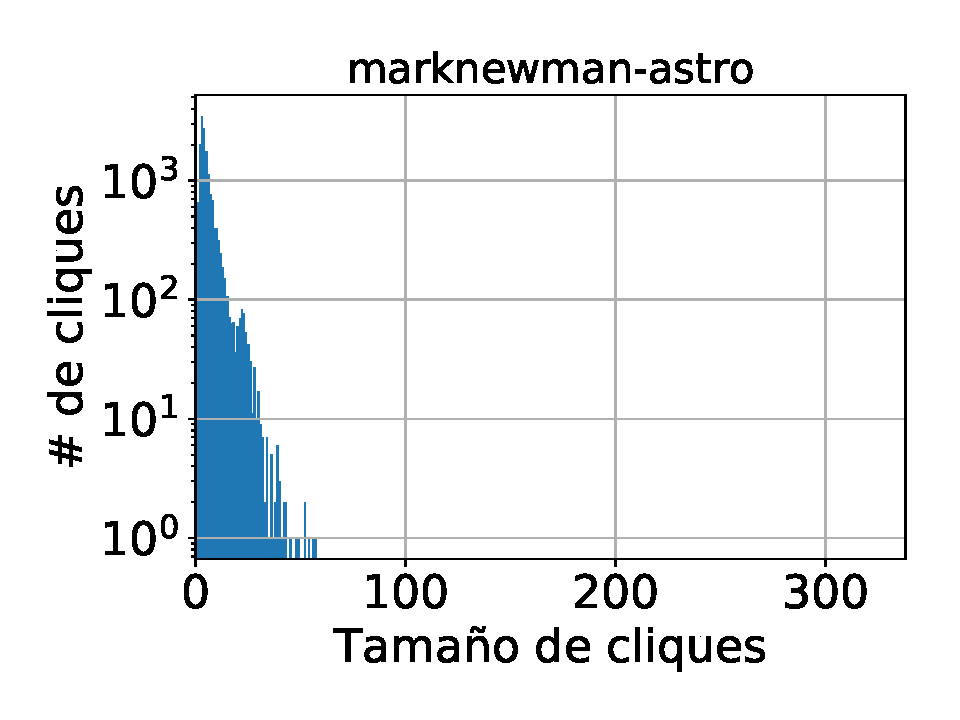
\includegraphics[width=1\linewidth]{../img/cliqueDist2/marknewman-astro.pdf}
    		\end{minipage}
    		\begin{minipage}{0.45\textwidth}
    			\centering
    			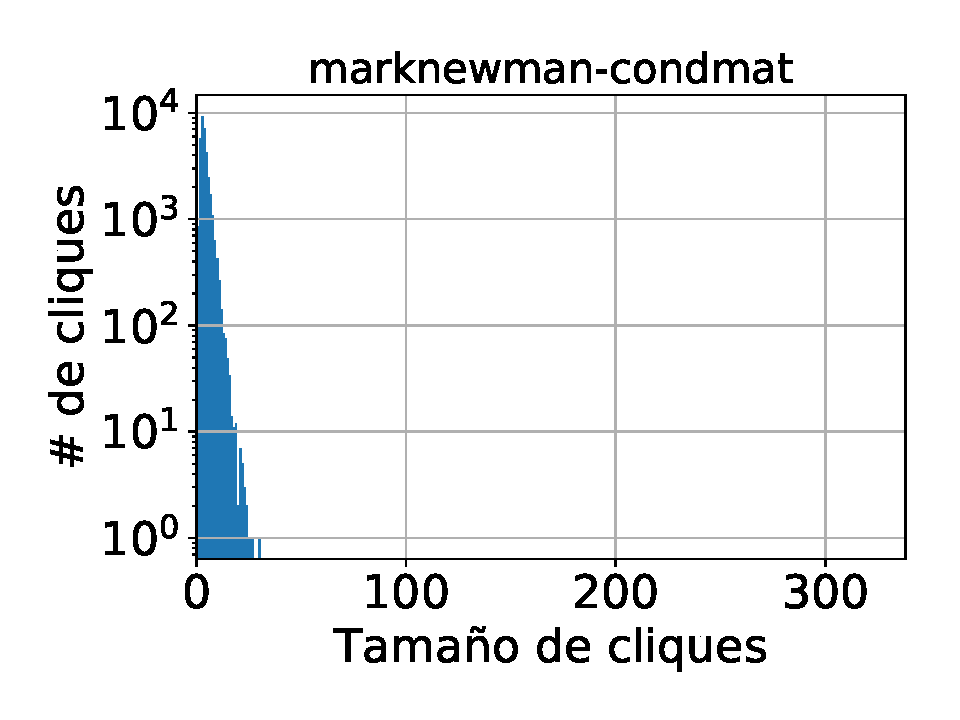
\includegraphics[width=1\linewidth]{../img/cliqueDist2/marknewman-condmat.pdf}
    		\end{minipage}  		
    	\end{minipage}
    	
    	\begin{minipage}{1\textwidth}
    		\centering
    		\begin{minipage}{0.45\textwidth}
    			\centering
    			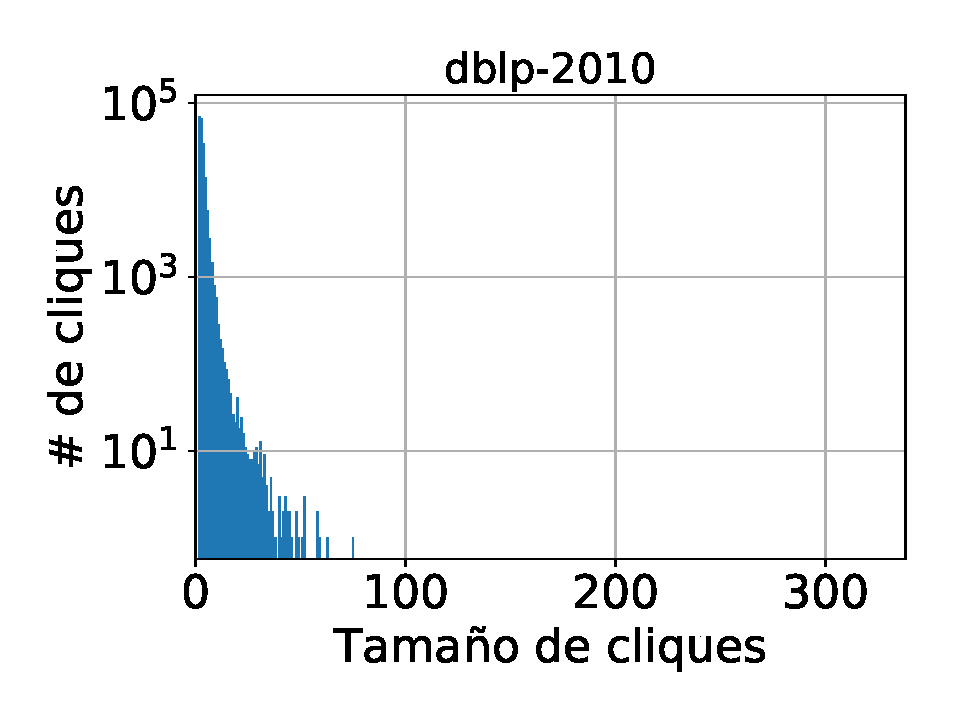
\includegraphics[width=1\linewidth]{../img/cliqueDist2/dblp-2010.pdf}
    		\end{minipage}
    		\begin{minipage}{0.45\textwidth}
    			\centering
    			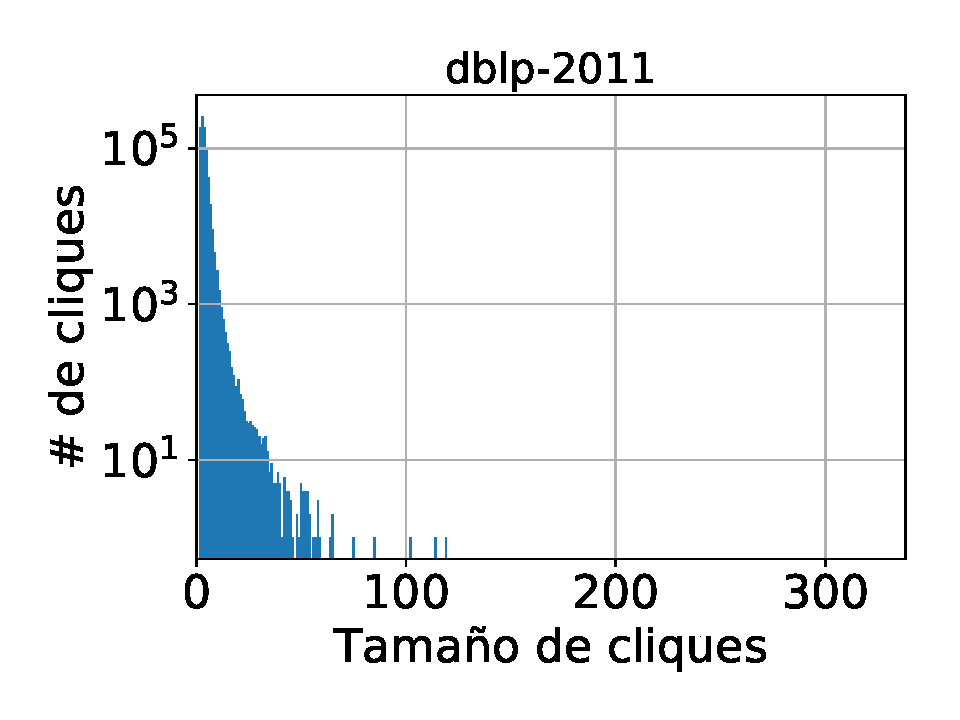
\includegraphics[width=1\linewidth]{../img/cliqueDist2/dblp-2011.pdf}
    		\end{minipage}  
    	\end{minipage}	

    \caption{Distribución del grado de los vértices para cada grafo (1).}
\end{figure}



\end{frame}
\begin{frame}%[noframenumbering]
\frametitle{Resultados - Distribución de tamaño de cliques}

\begin{figure}
    \centering
    	\begin{minipage}{1\textwidth}
    		\centering
    		\begin{minipage}{0.45\textwidth}
    			\centering
    			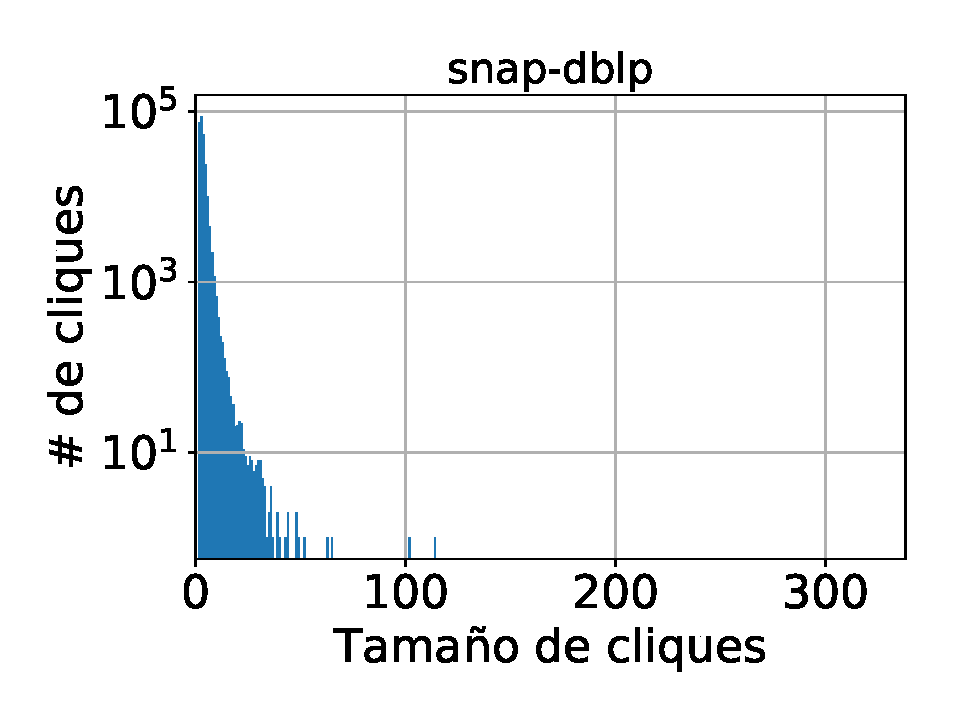
\includegraphics[width=1\linewidth]{../img/cliqueDist2/snap-dblp.pdf}
    		\end{minipage}
    		\begin{minipage}{0.45\textwidth}
    			\centering
    			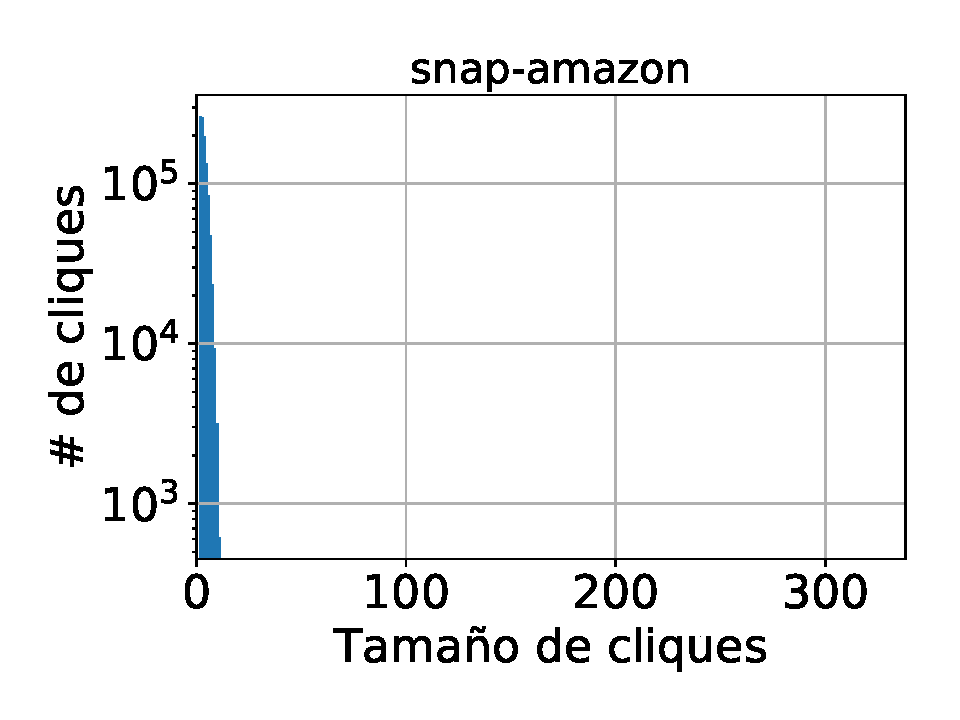
\includegraphics[width=1\linewidth]{../img/cliqueDist2/snap-amazon.pdf}
    		\end{minipage}  		
    	\end{minipage}
    	
    	\begin{minipage}{1\textwidth}
    		\centering
    		\begin{minipage}{0.45\textwidth}
    			\centering
    			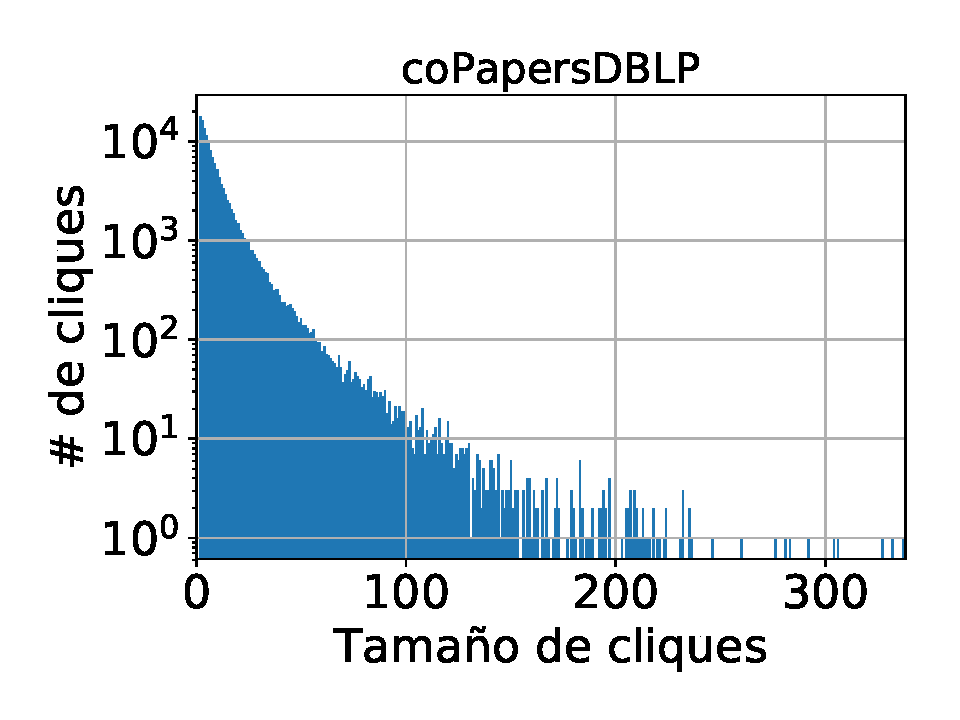
\includegraphics[width=1\linewidth]{../img/cliqueDist2/coPapersDBLP.pdf}
    		\end{minipage}
    		\begin{minipage}{0.45\textwidth}
    			\centering
    			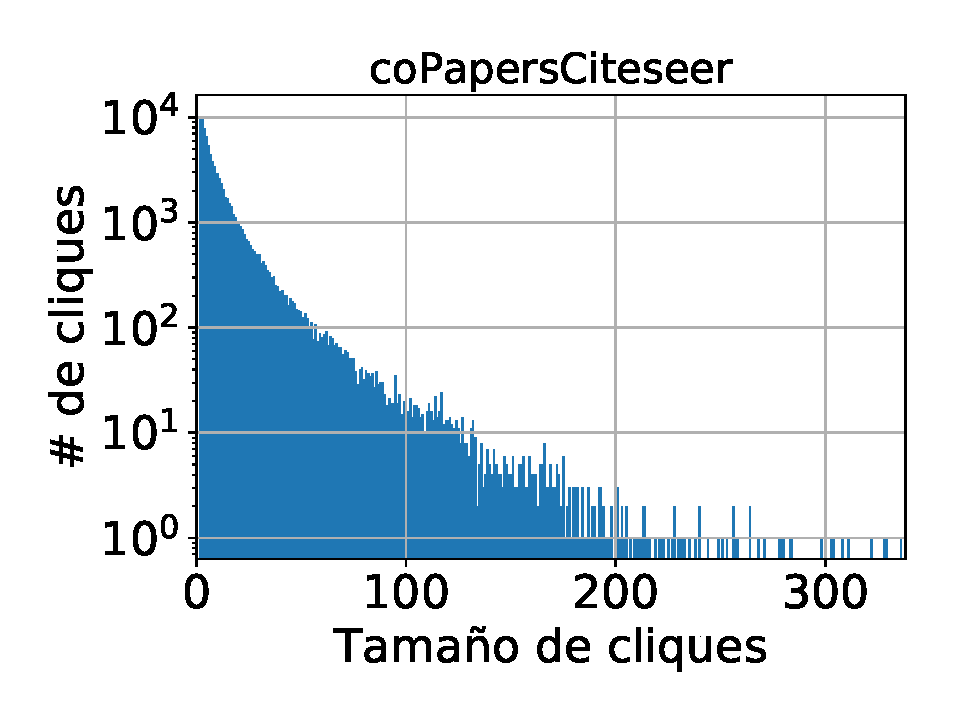
\includegraphics[width=1\linewidth]{../img/cliqueDist2/coPapersCiteseer.pdf}
    		\end{minipage}  
    	\end{minipage}	

    \caption{Distribución del grado de los vértices para cada grafo (2).}
\end{figure}

\end{frame}



\begin{frame}
\frametitle{Resultados - Funciones de ranking}

\begin{figure}
    	\centering
    	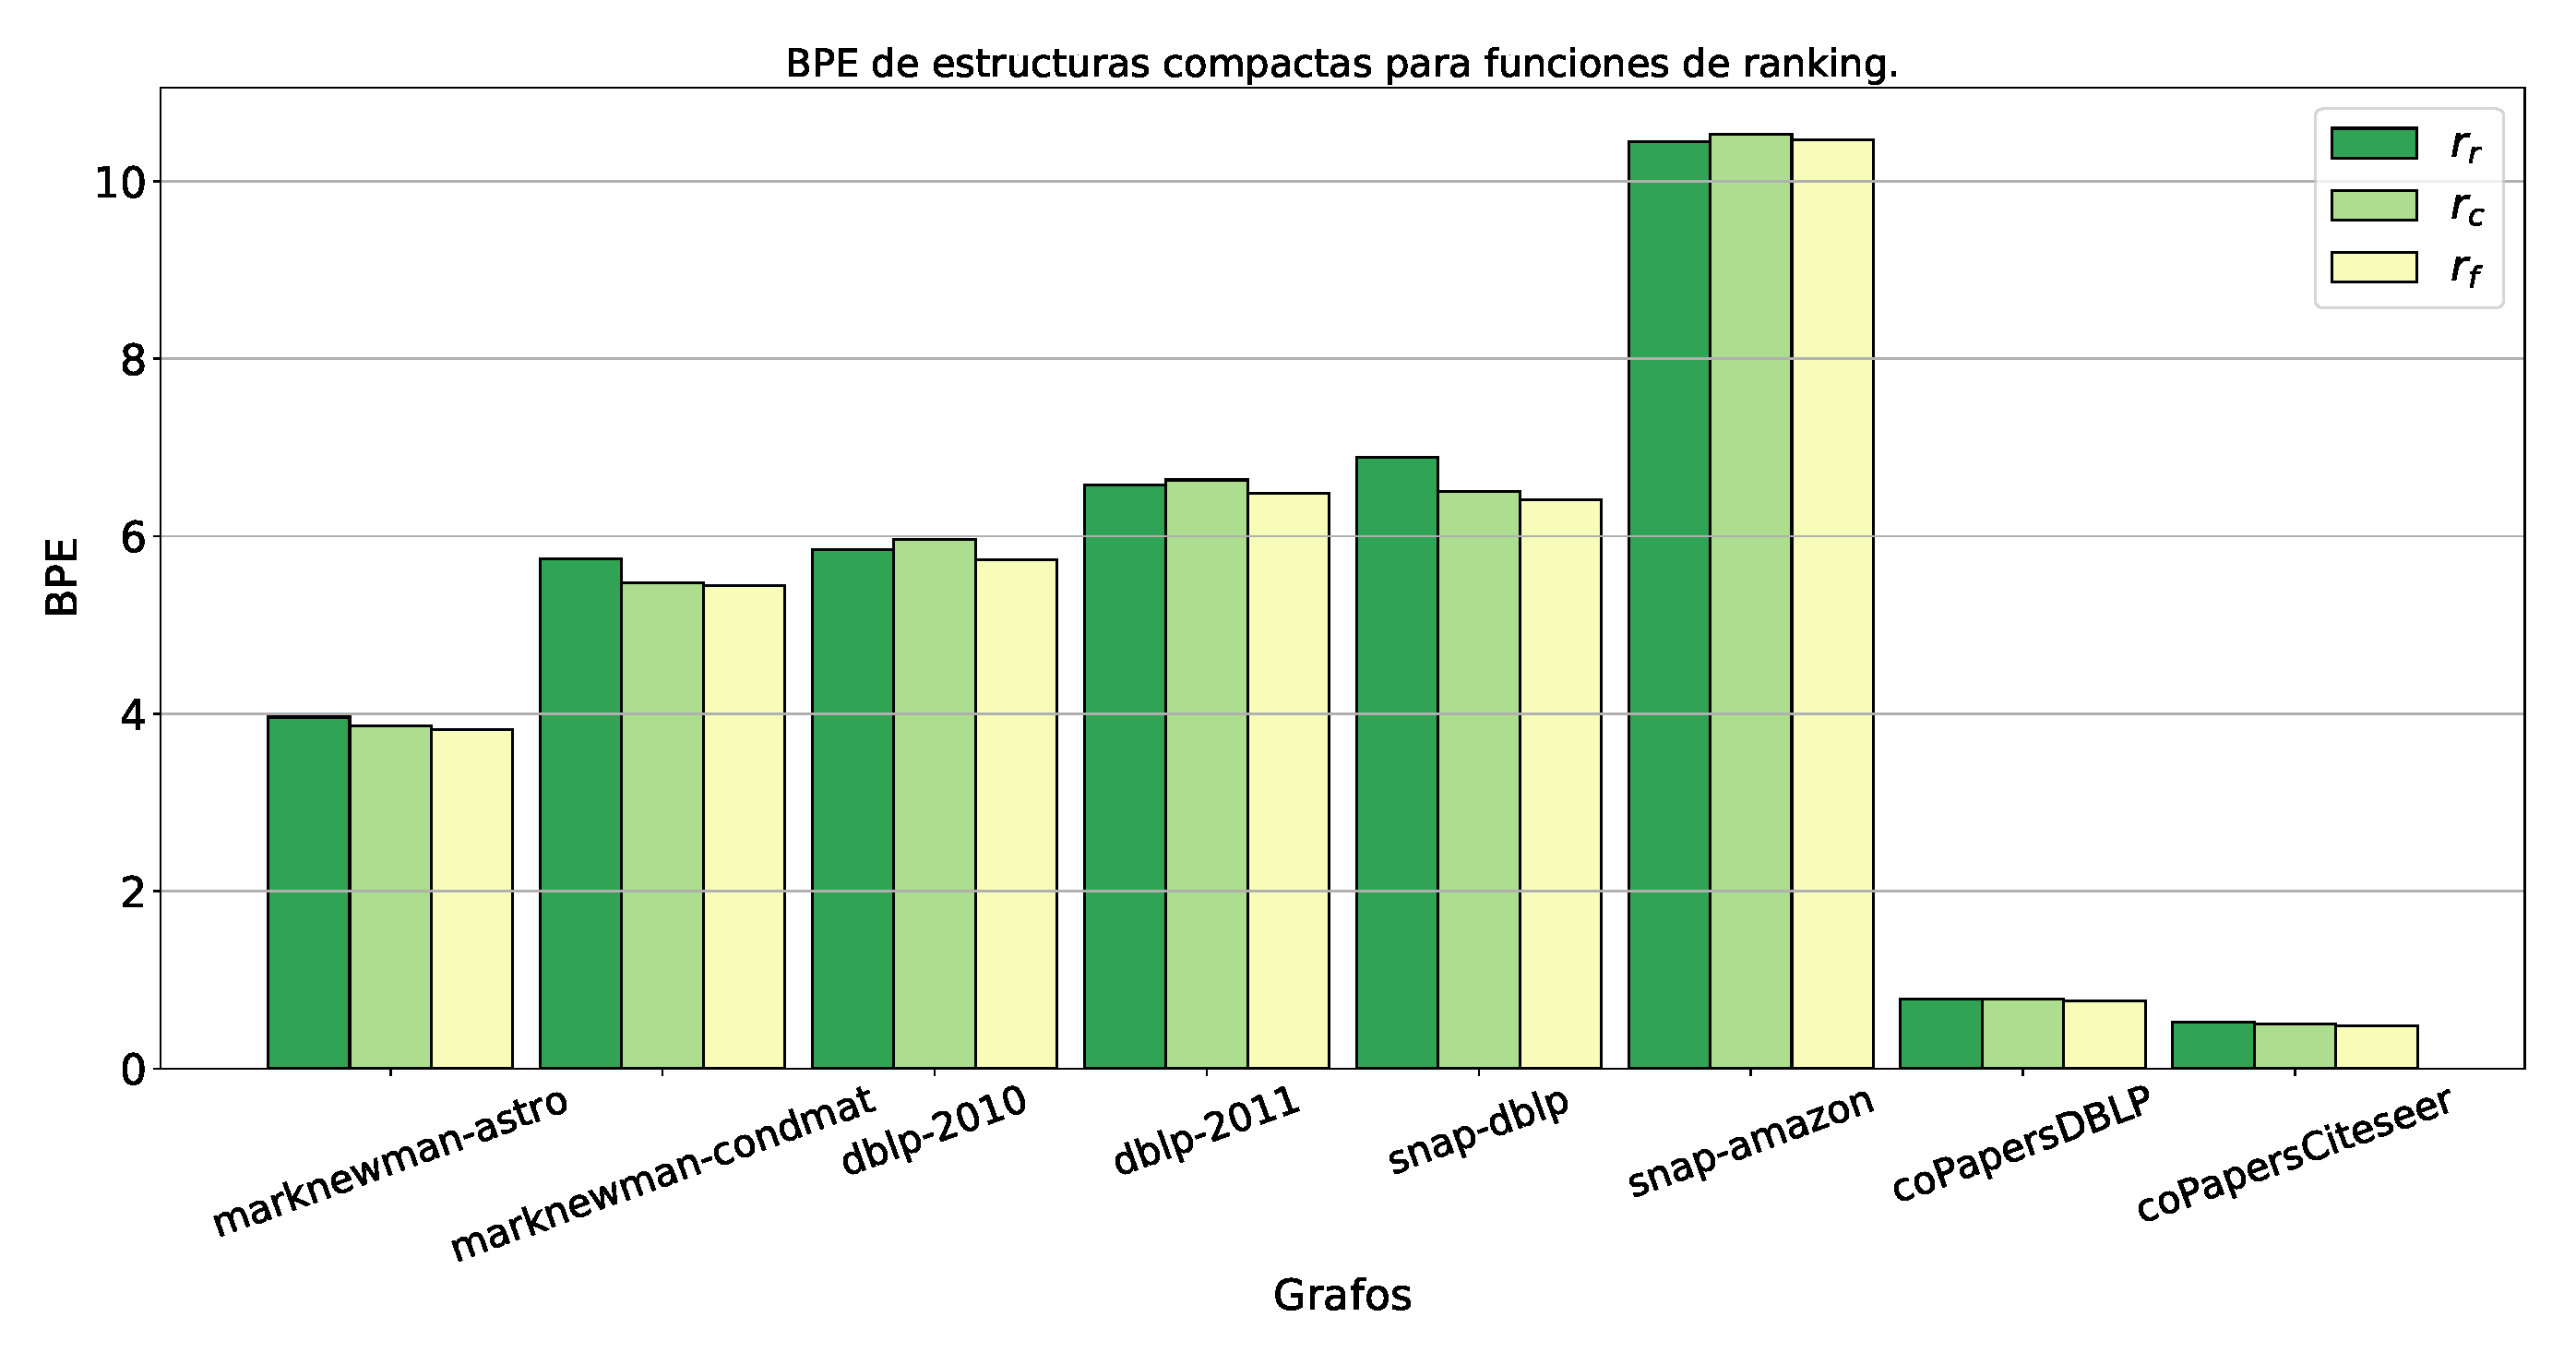
\includegraphics[width=1\linewidth]{../img/bpe3.pdf}
    	
    \caption{BPE de las estructuras compactas para las funciones de ranking.}
\end{figure}

\end{frame}


\begin{frame}
\frametitle{Resultados - Funciones de ranking}

\begin{figure}
    	\centering
    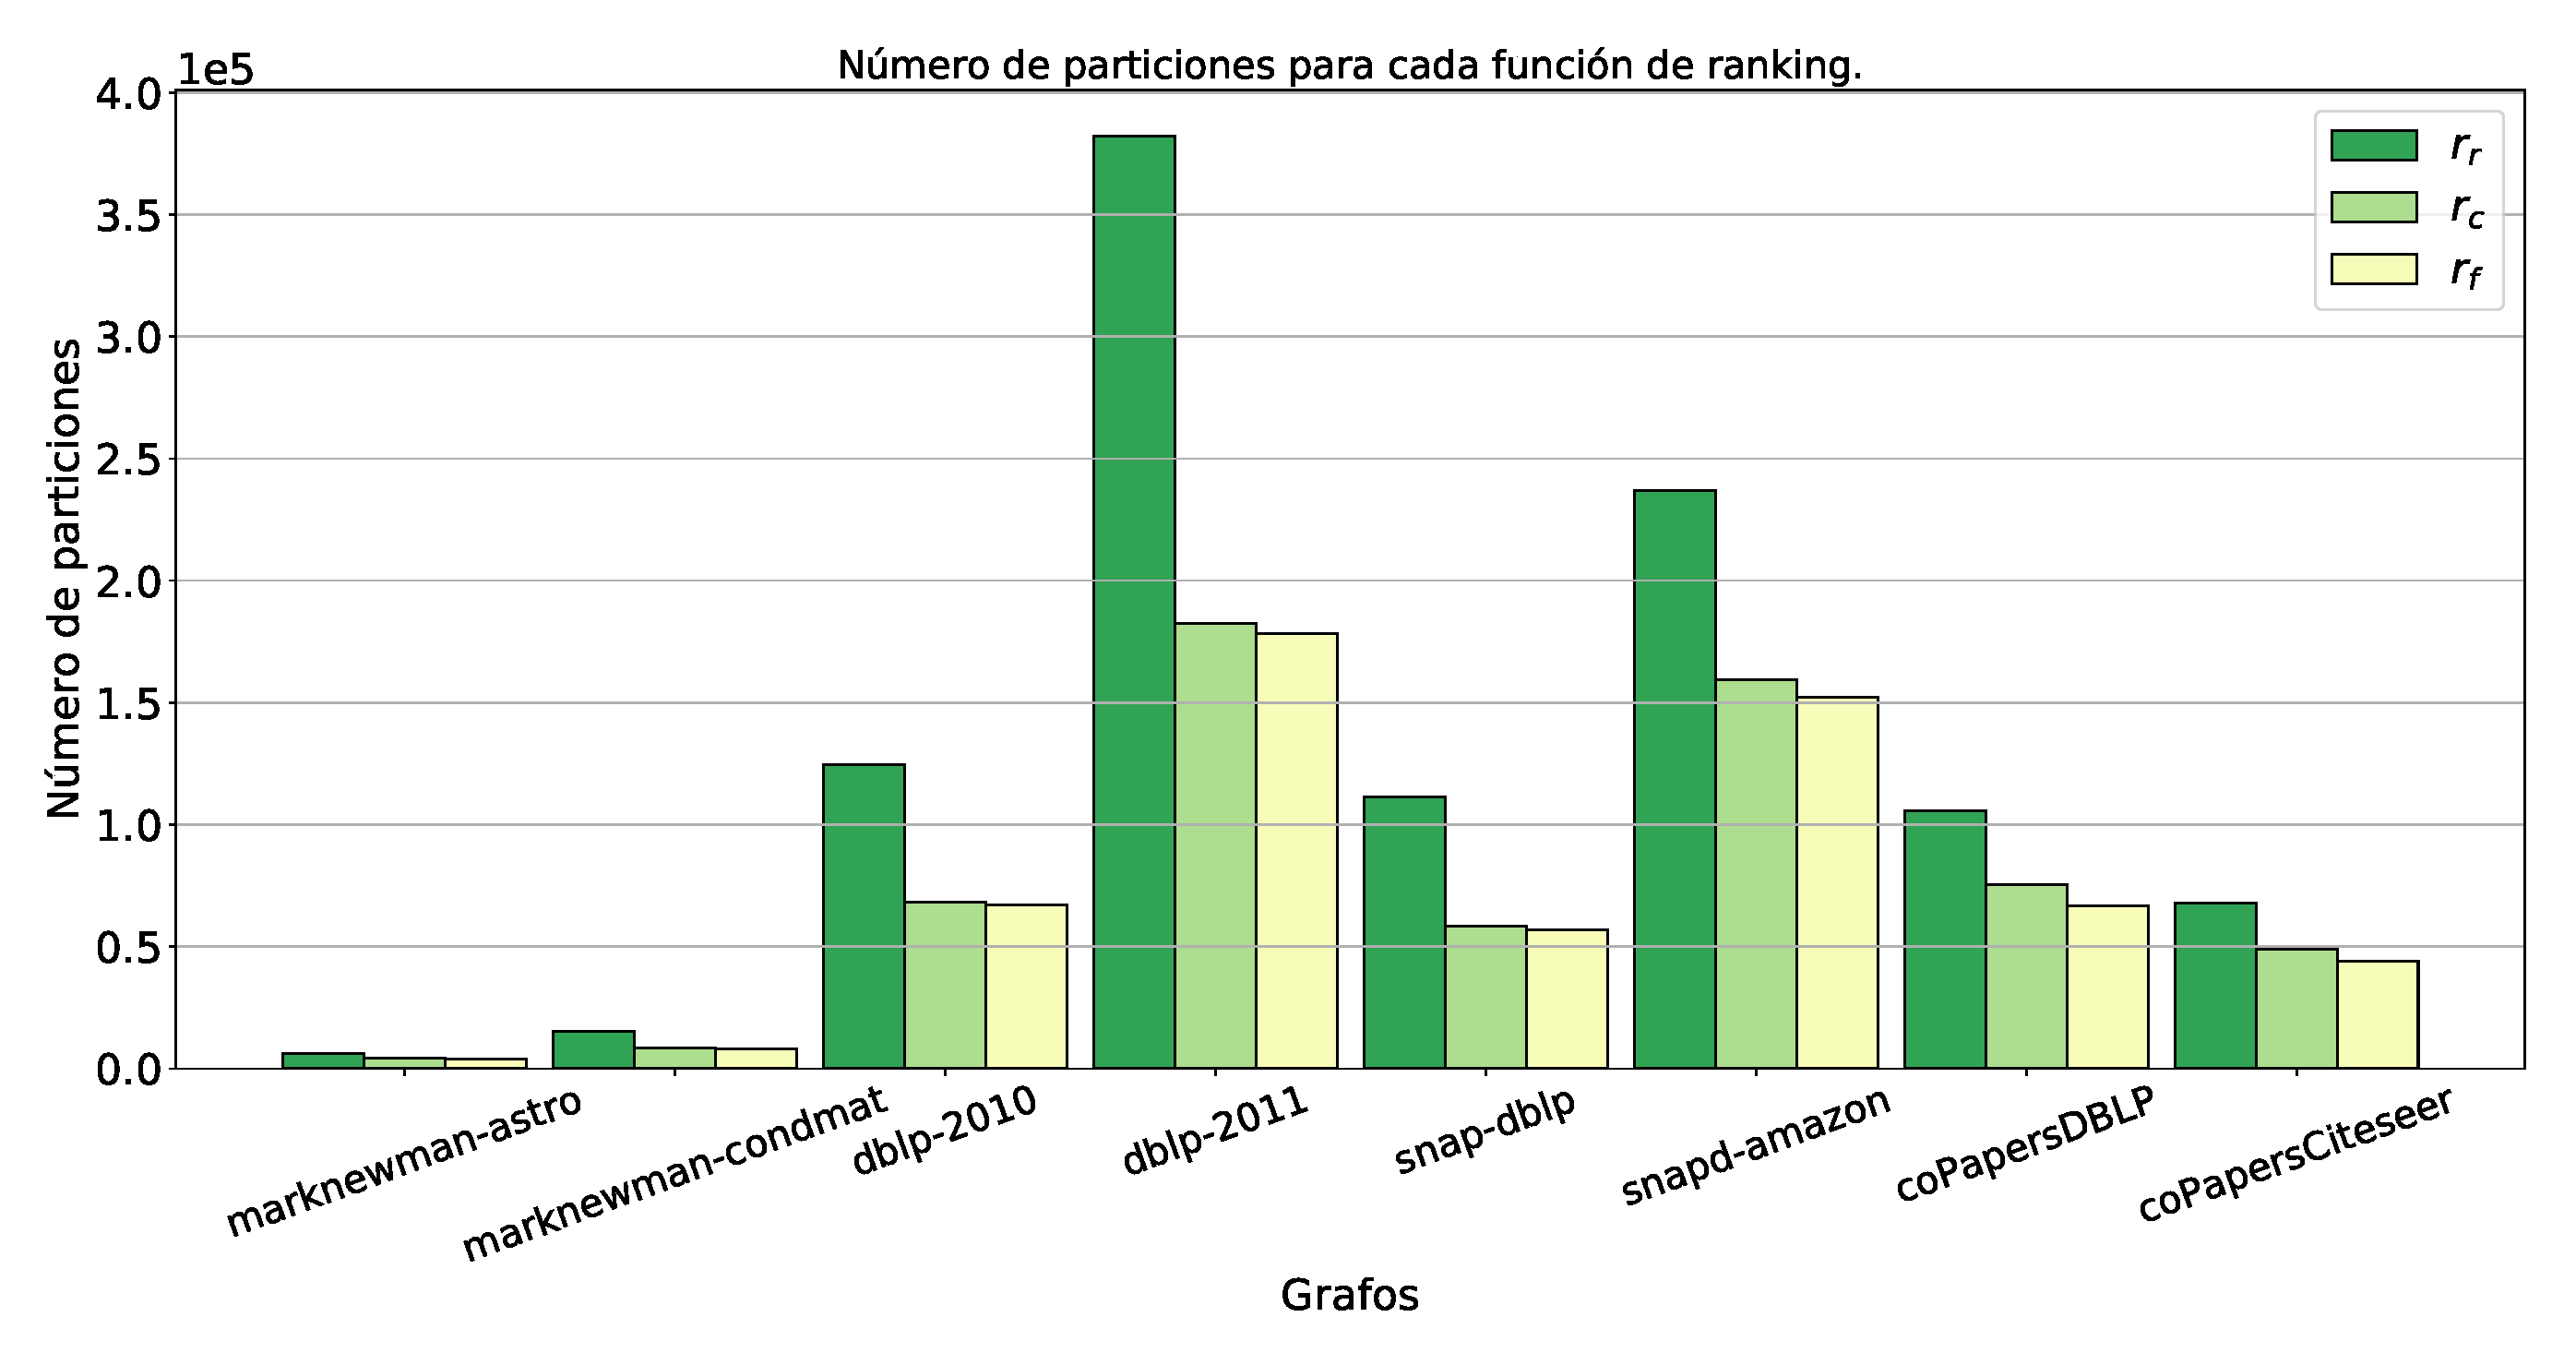
\includegraphics[width=1\linewidth]{../img/Npartitions3.pdf}
    	
    \caption{Número de particiones en las estructuras compactas para las funciones de ranking.}
\end{figure}

\end{frame}

\begin{frame}
\frametitle{Resultados - Funciones de ranking}

\begin{figure}
    	\centering
    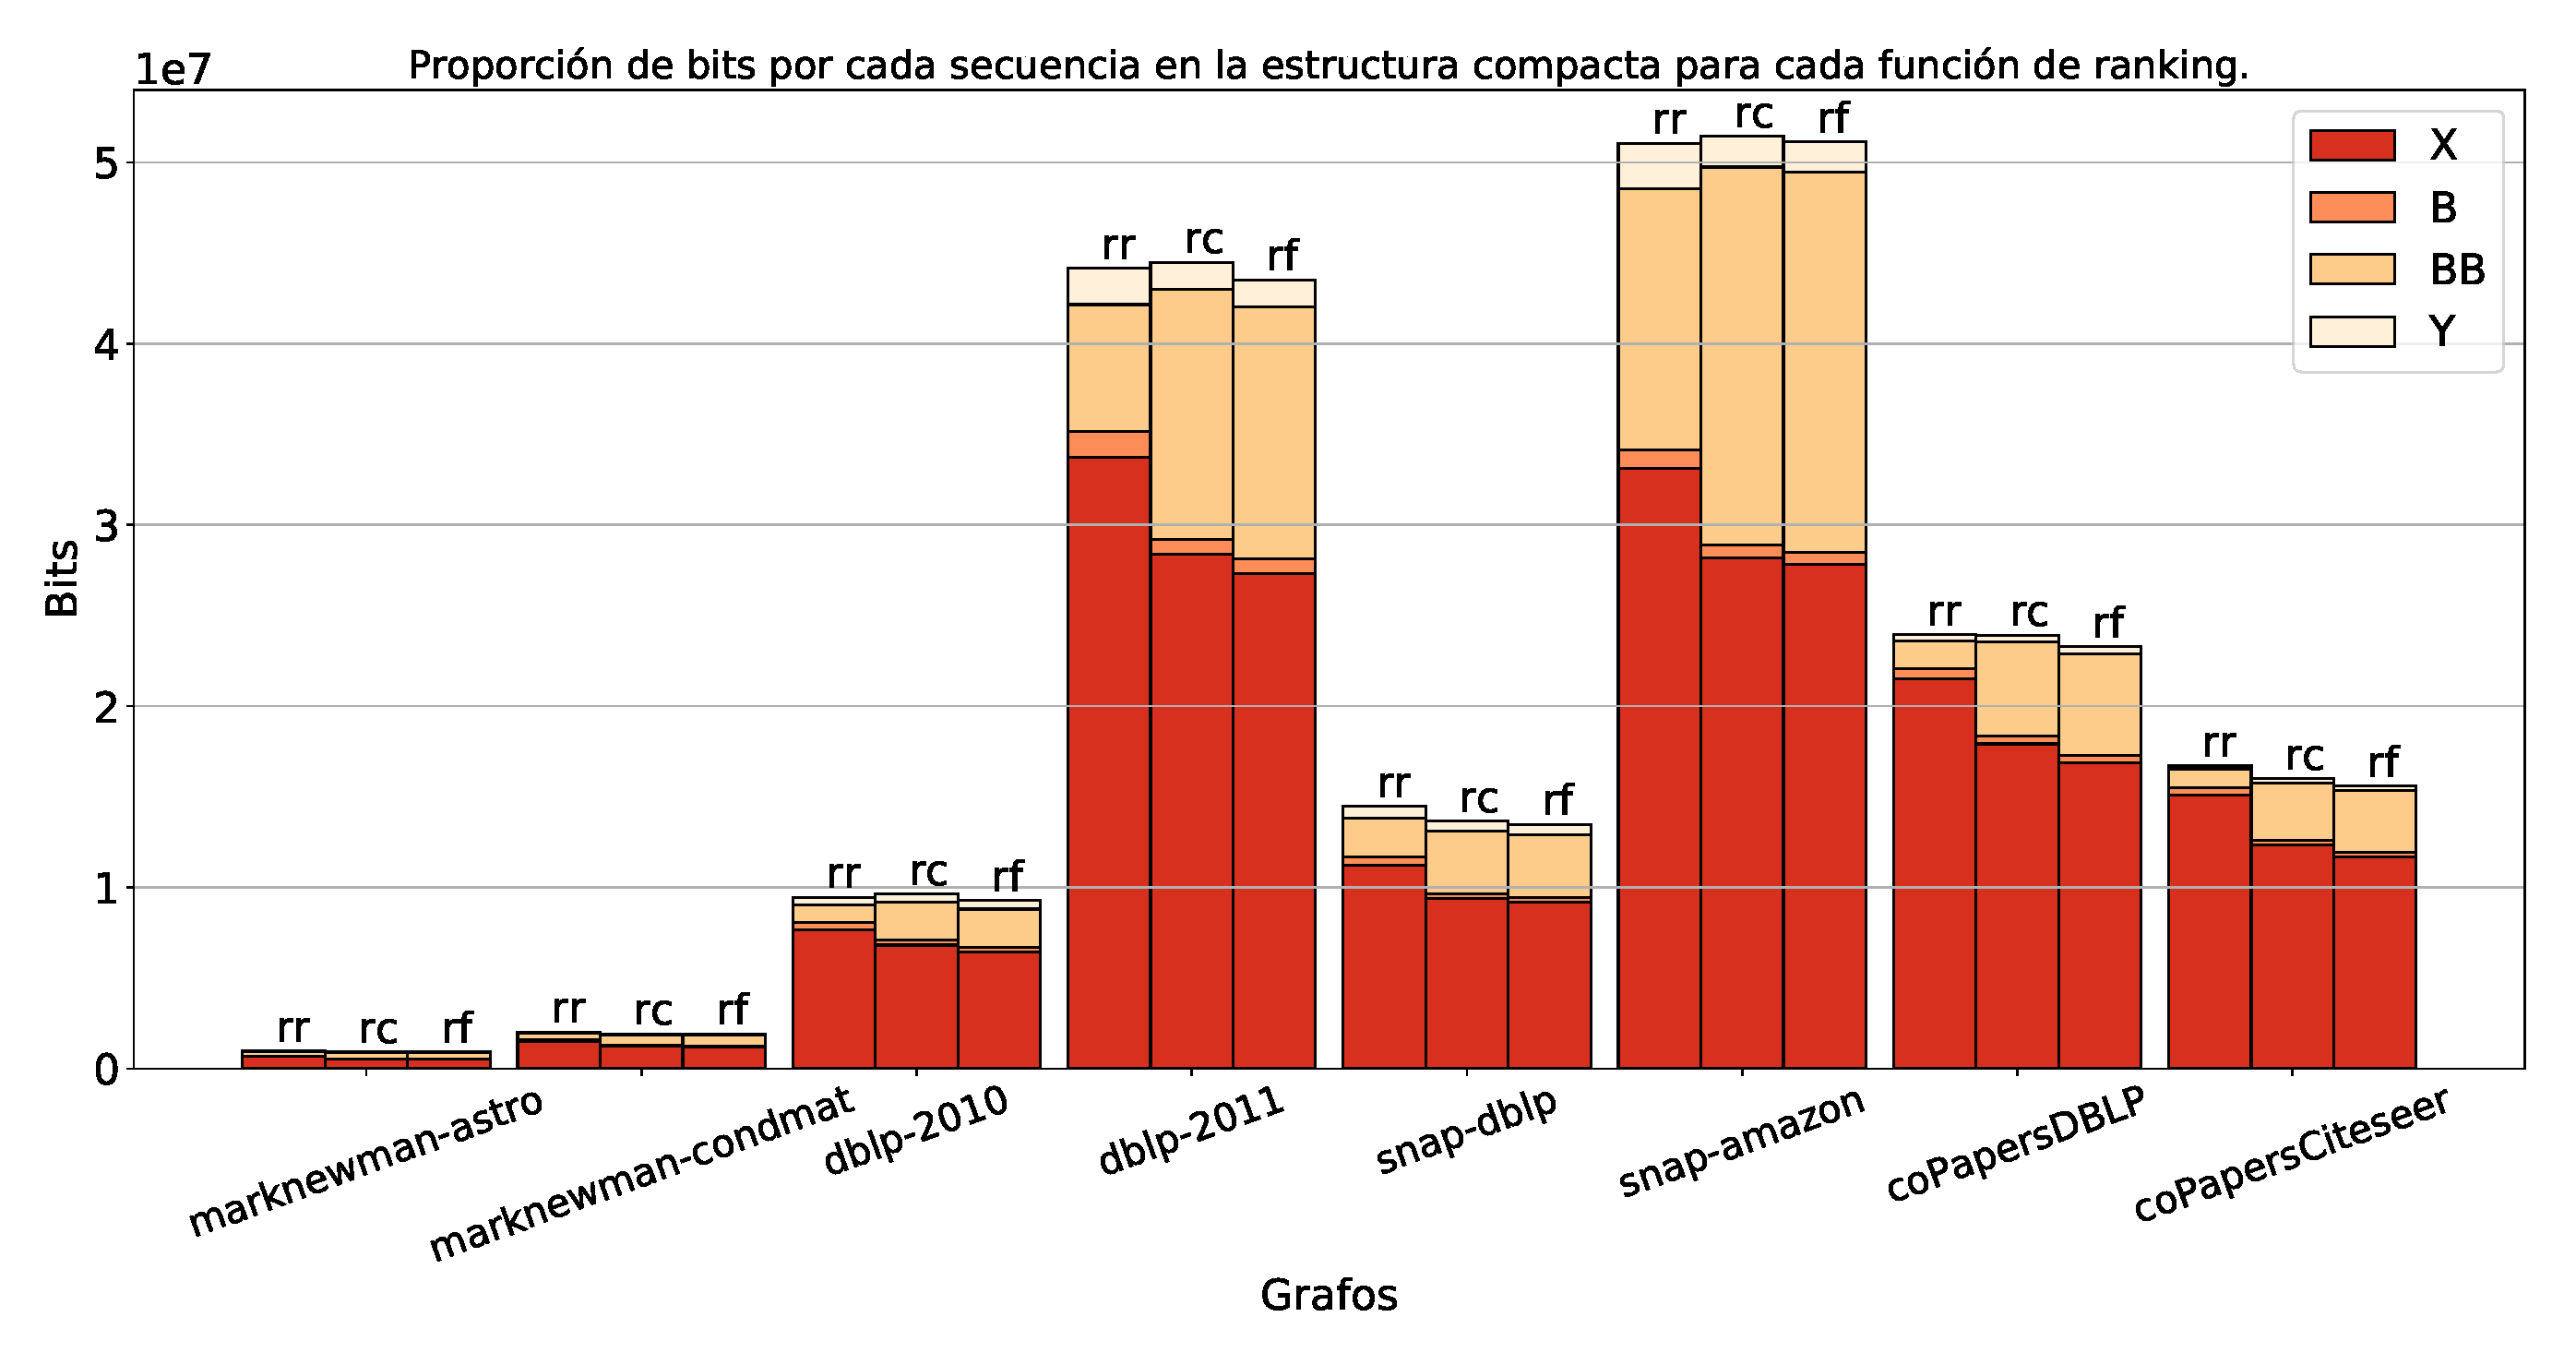
\includegraphics[width=1\linewidth]{../img/bits.pdf}
    	
    \caption{Proporción de bits por cada secuencia en la estructura compacta, para cada función de ranking}
\end{figure}

\end{frame}

\begin{frame}
\frametitle{Resultados - Funciones de ranking}

\begin{figure}
    	\centering
    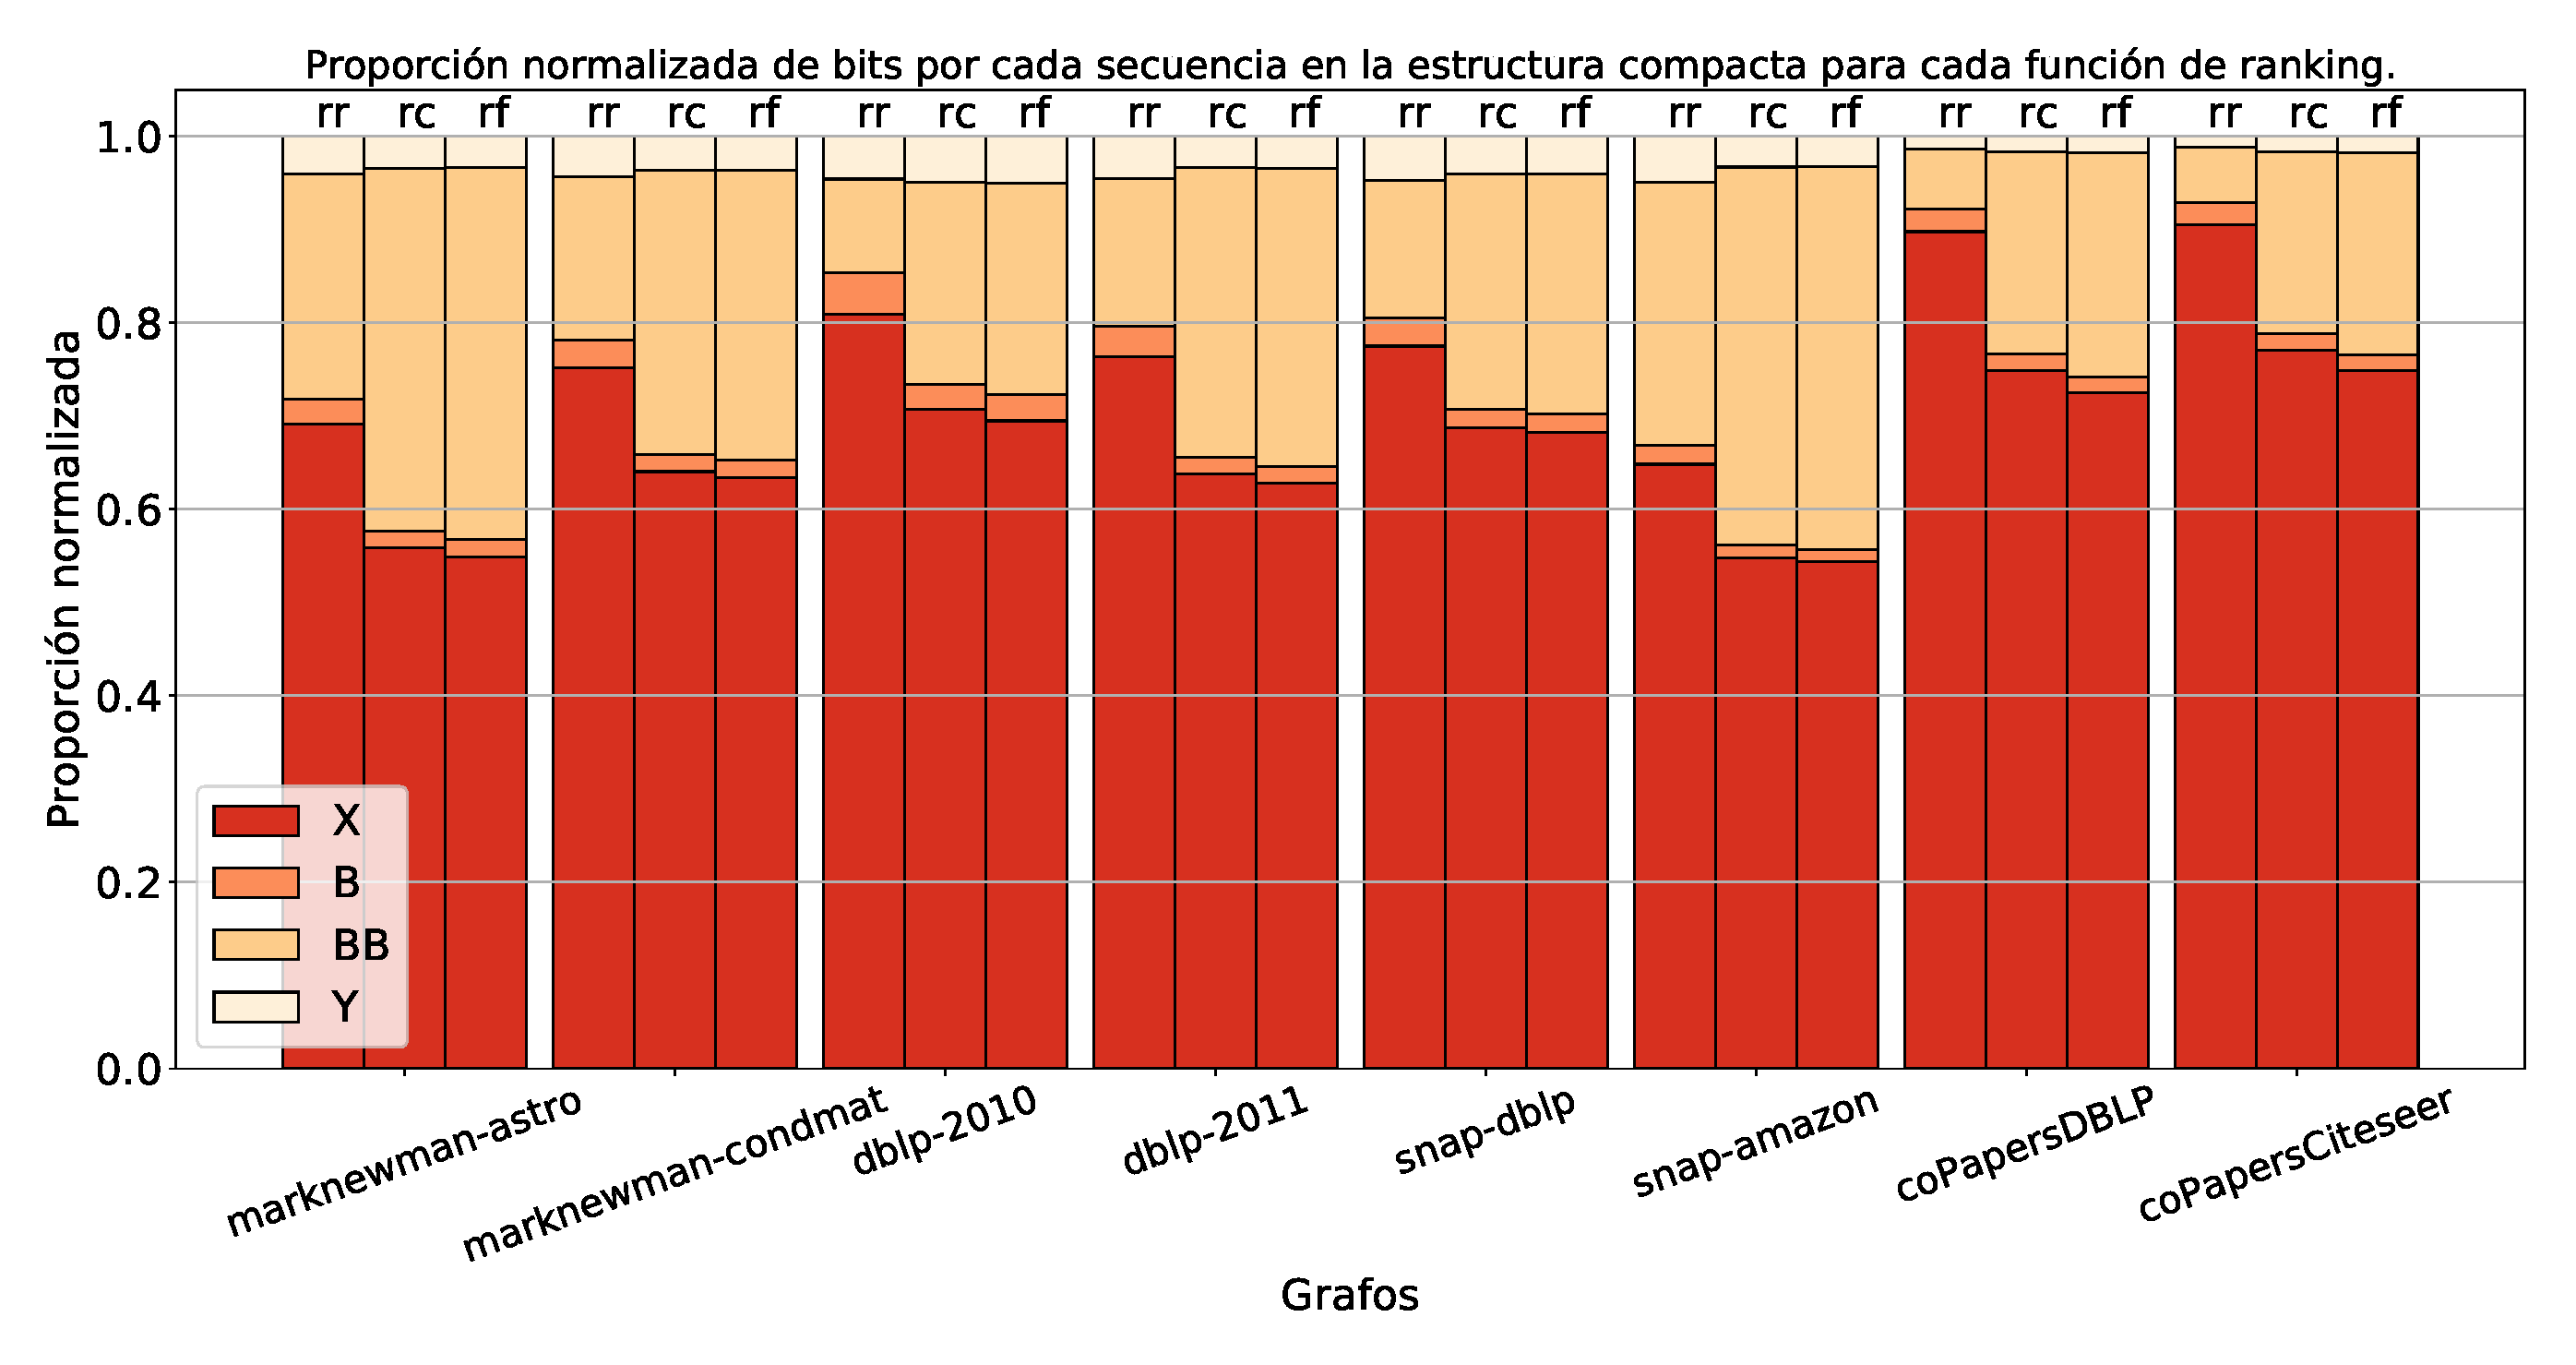
\includegraphics[width=1\linewidth]{../img/bitsNorm.pdf}
    	
    \caption{Proporción normalizada de bits por cada secuencia en la estructura compacta, para cada función de ranking}
\end{figure}

\end{frame}


\begin{frame}
\frametitle{Resultados - Funciones de ranking}

\begin{figure}
    	\centering
    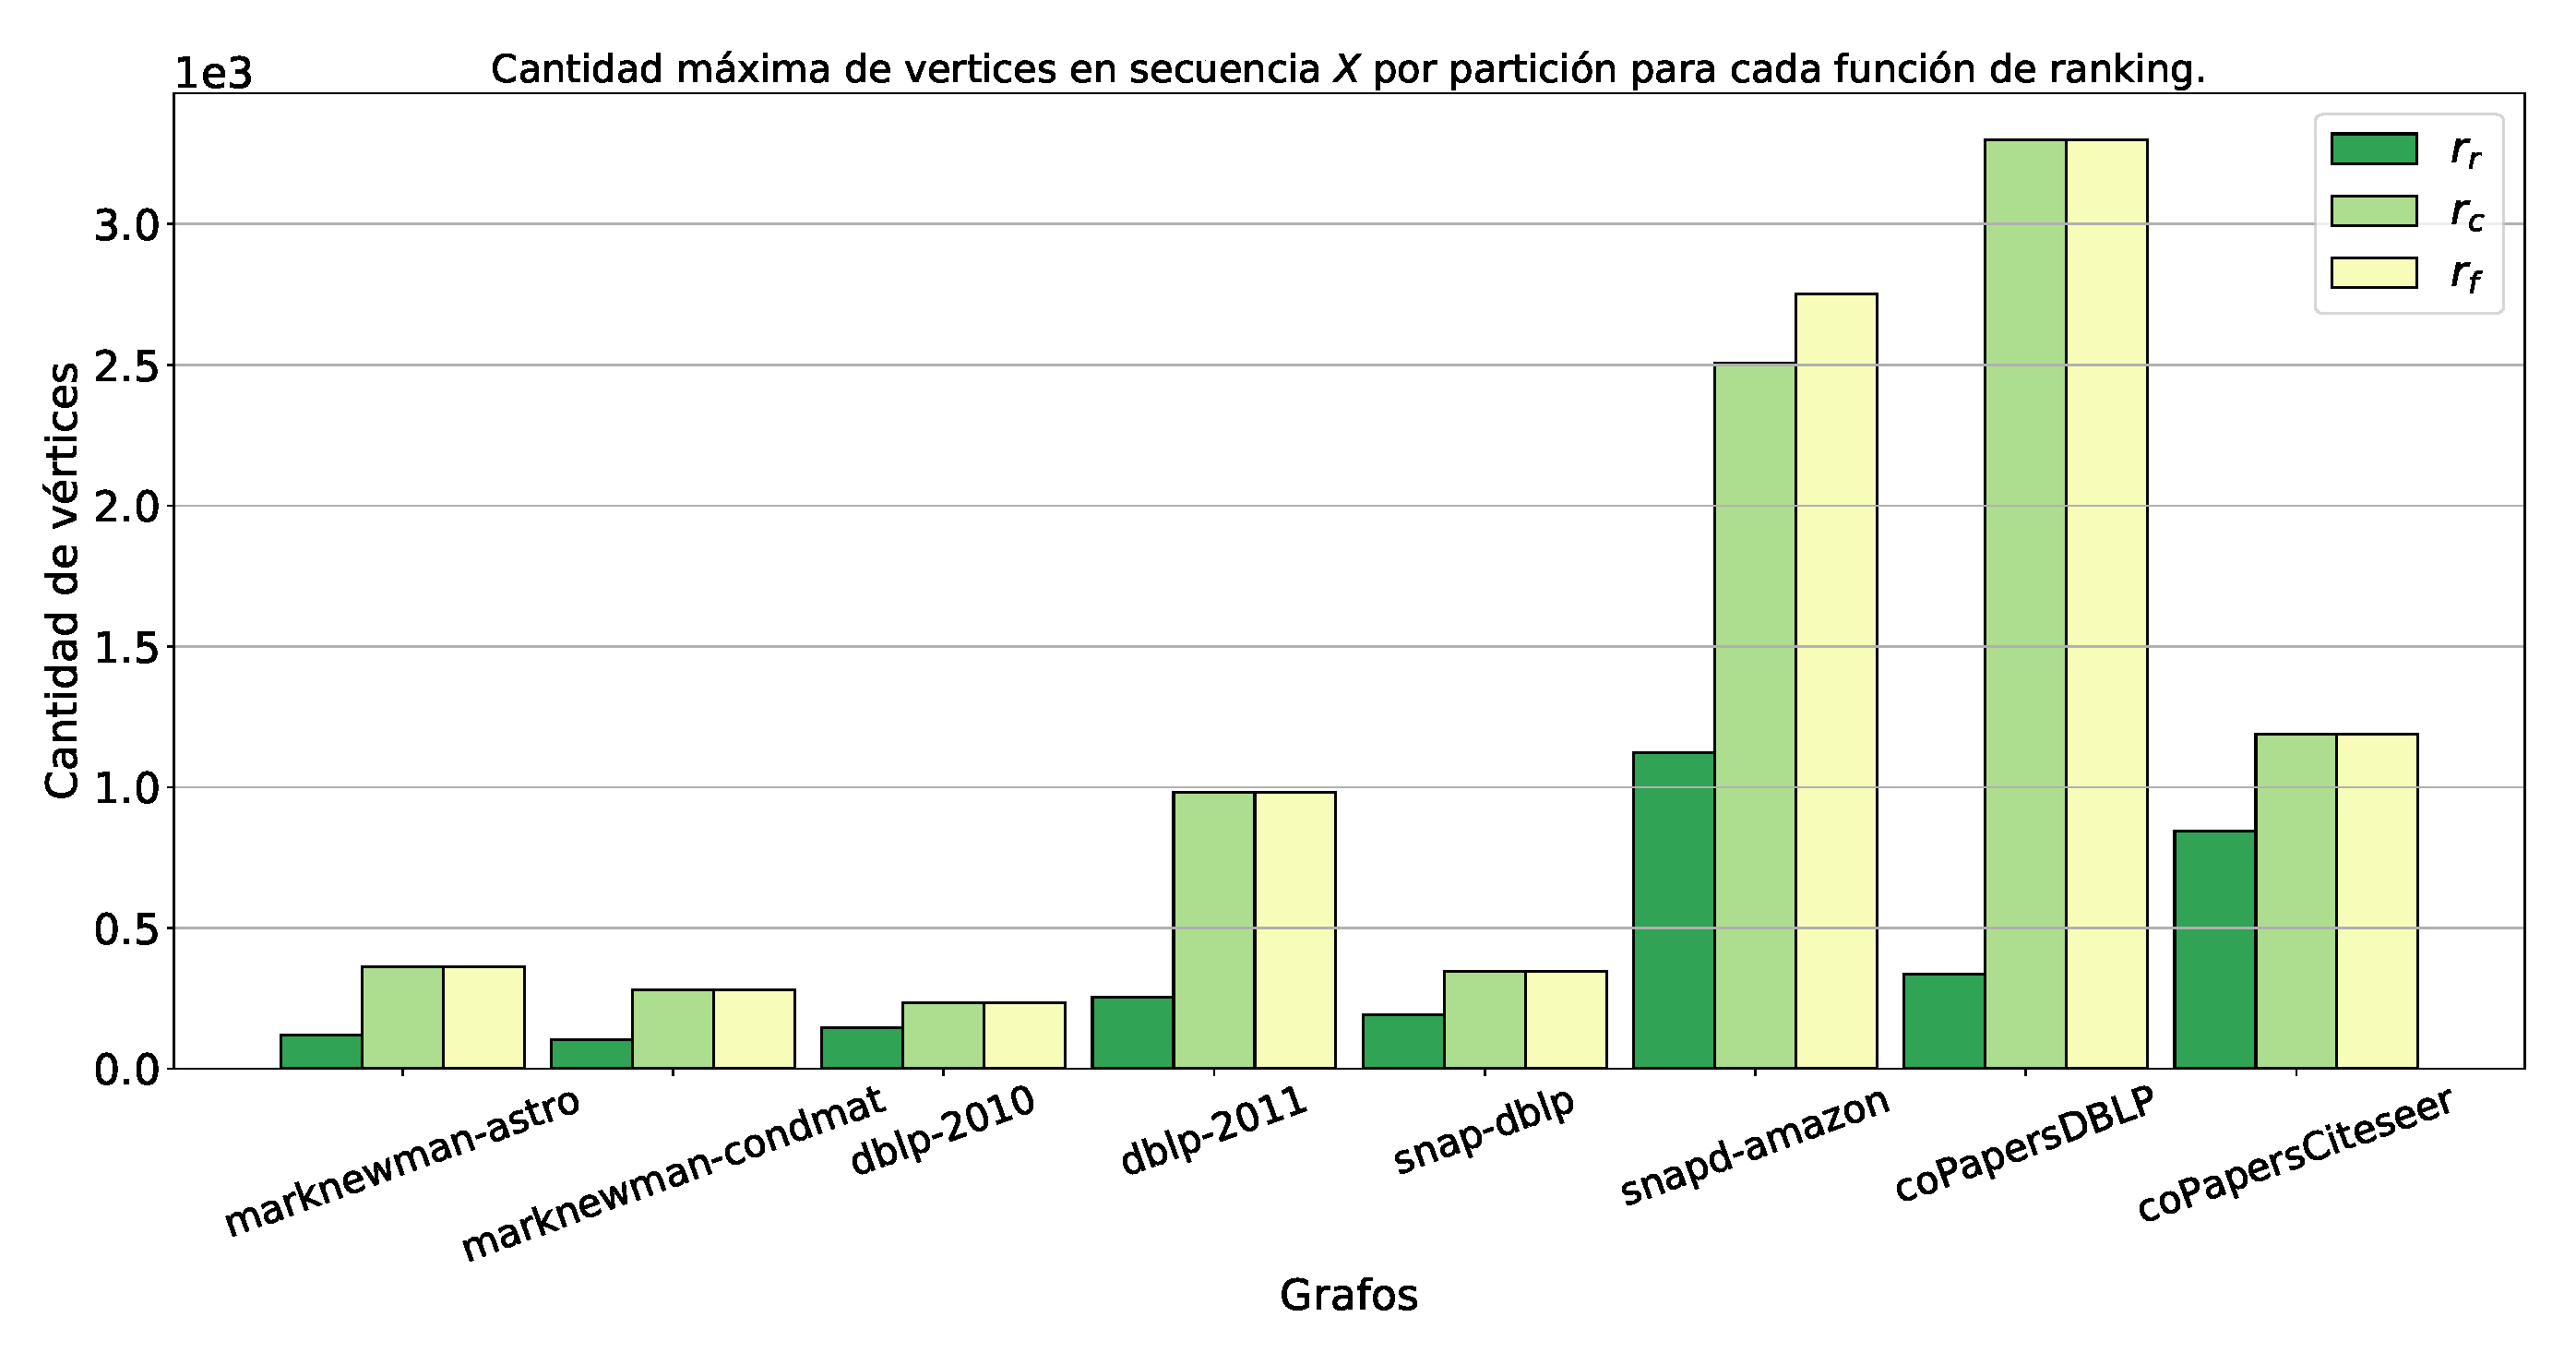
\includegraphics[width=1\linewidth]{../img/maxNodes.pdf}
    	
    \caption{Número máximo de vértices en la secuencia $X$ para las funciones de ranking.}
\end{figure}

\end{frame}

\begin{frame}
\frametitle{Resultados - Funciones de ranking}

\begin{figure}
    	\centering
    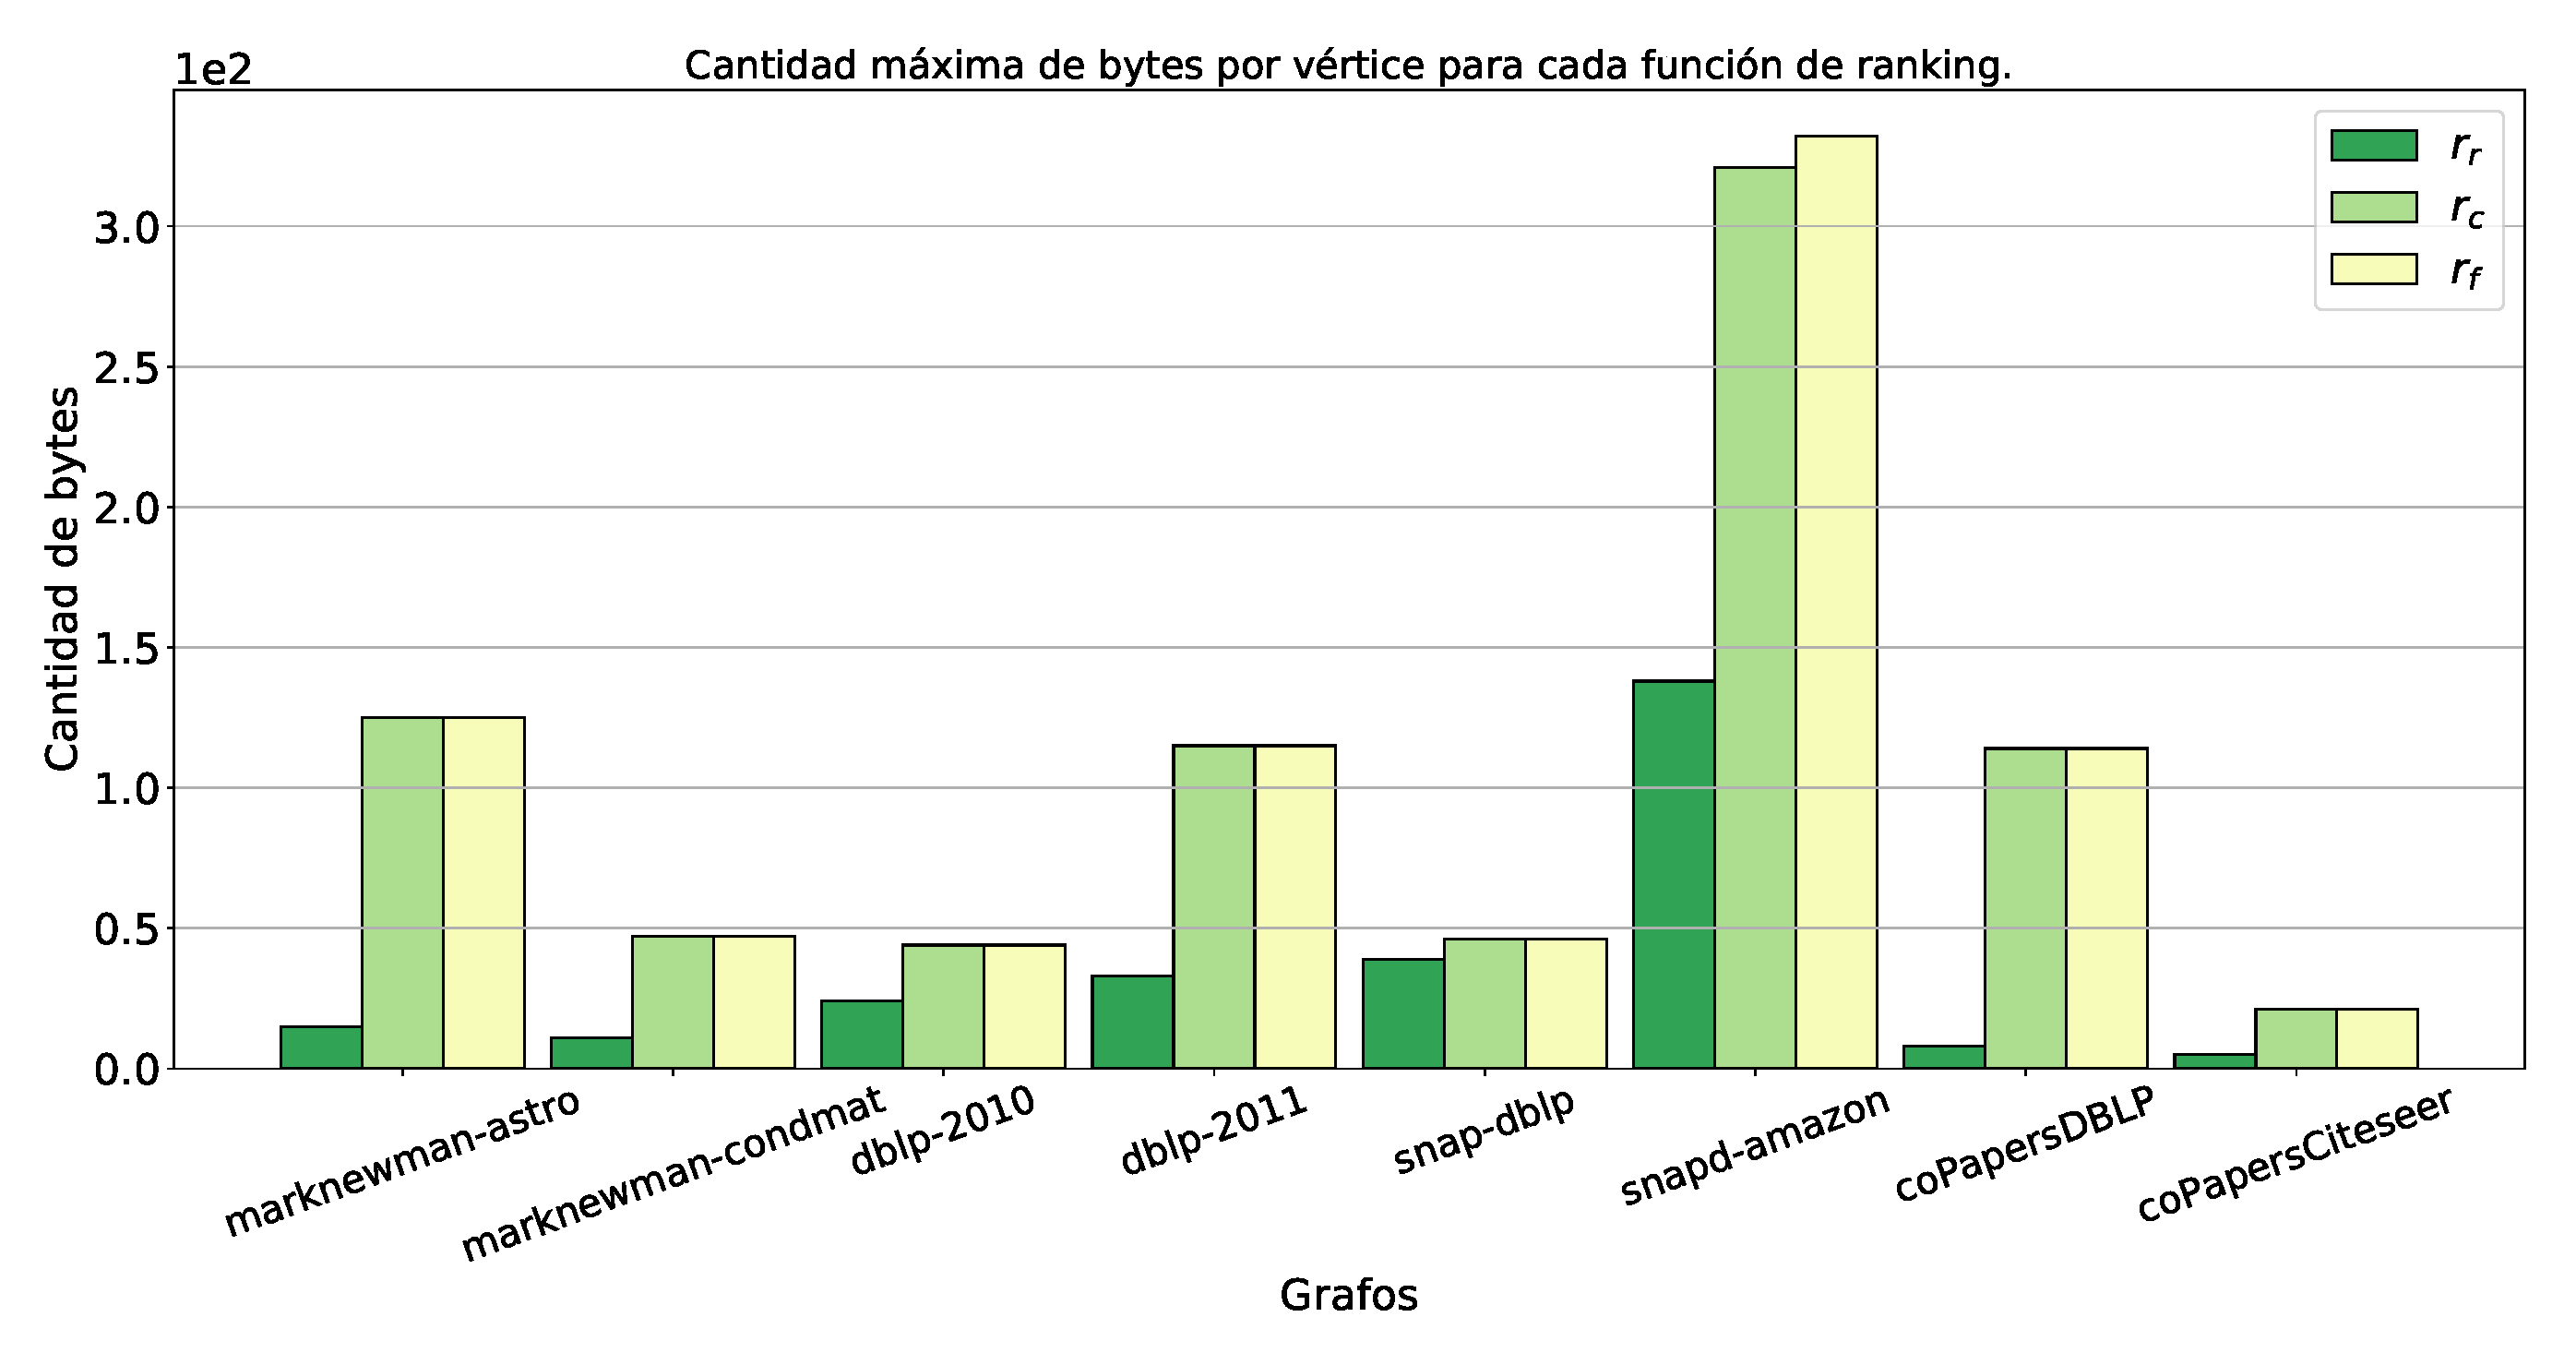
\includegraphics[width=1\linewidth]{../img/maxBytes.pdf}
    	
    \caption{Número máximo de bytes por nodo para las funciones de ranking.}
\end{figure}

\end{frame}



\begin{frame}
\frametitle{Resultados - Funciones de ranking}

\begin{figure}
    \centering
    	\begin{minipage}{1\textwidth}
    		\centering
    		\begin{minipage}{0.45\textwidth}
    			\centering
    			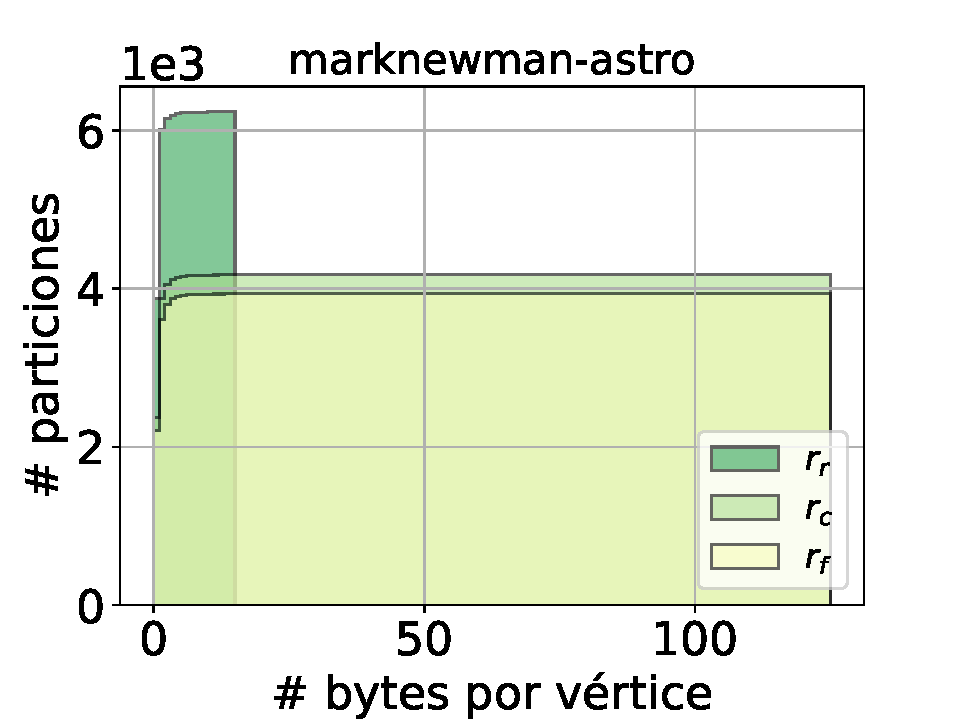
\includegraphics[width=1\linewidth]{../img/cdf/marknewman-astro.pdf}
    		\end{minipage}
    		\begin{minipage}{0.45\textwidth}
    			\centering
    			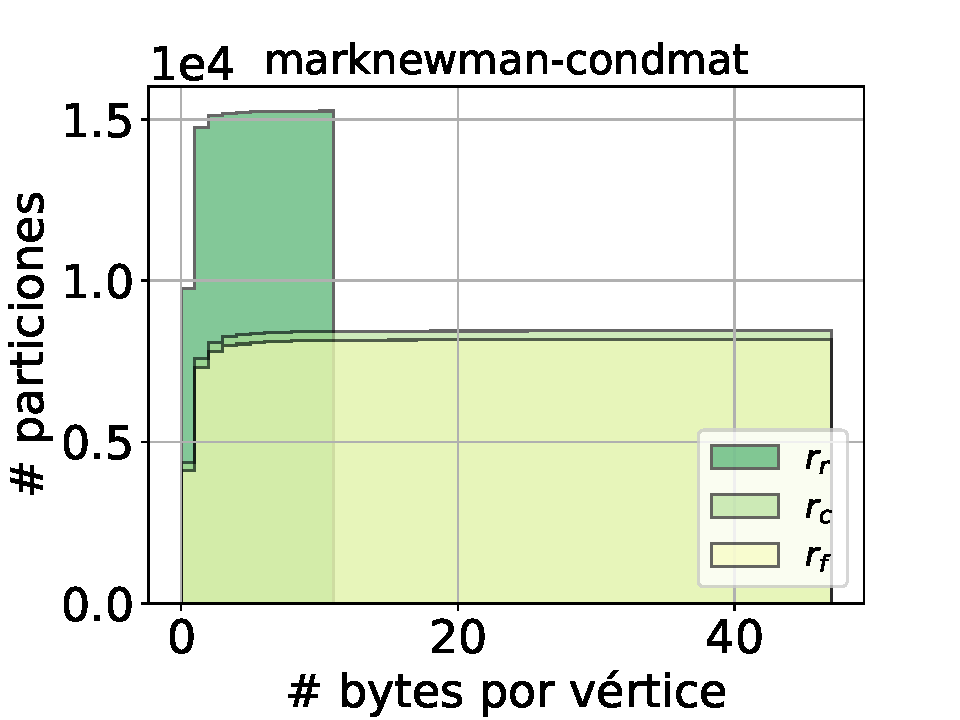
\includegraphics[width=1\linewidth]{../img/cdf/marknewman-condmat.pdf}
    		\end{minipage}  		
    	\end{minipage}
    	
    	\begin{minipage}{1\textwidth}
    		\centering
    		\begin{minipage}{0.45\textwidth}
    			\centering
    			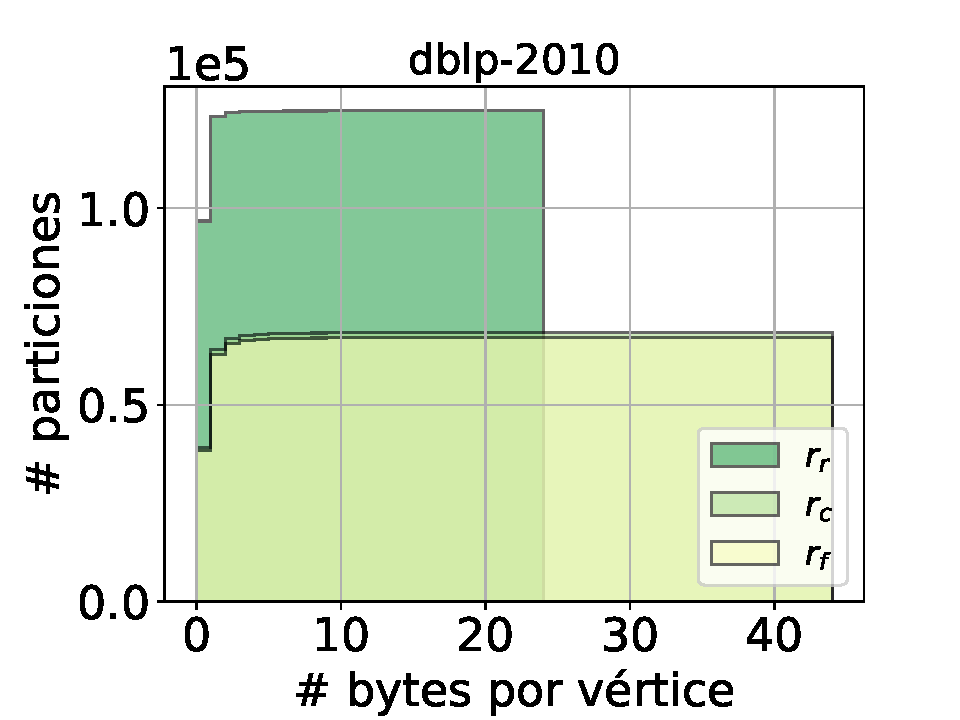
\includegraphics[width=1\linewidth]{../img/cdf/dblp-2010.pdf}
    		\end{minipage}
    		\begin{minipage}{0.45\textwidth}
    			\centering
    			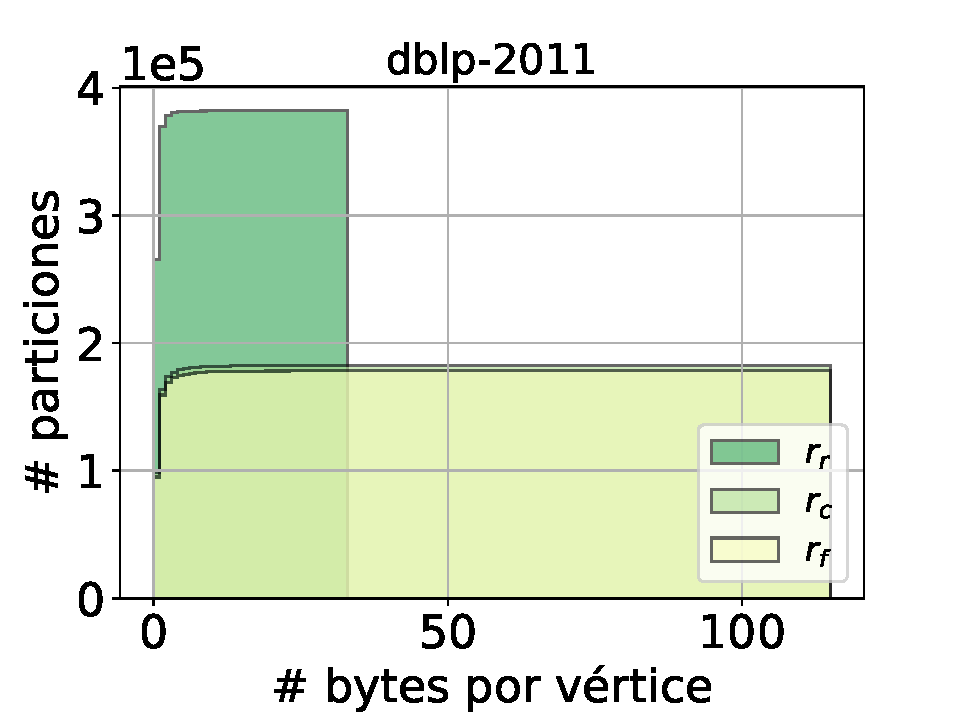
\includegraphics[width=1\linewidth]{../img/cdf/dblp-2011.pdf}
    		\end{minipage}  
    	\end{minipage}	

    \caption{CDF para bytes por vértice en estructuras compactas para cada función de ranking (1).}
\end{figure}


\end{frame}
\begin{frame}%[noframenumbering]
\frametitle{Resultados - Funciones de ranking}

\begin{figure}
    \centering
    	\begin{minipage}{1\textwidth}
    		\centering
    		\begin{minipage}{0.45\textwidth}
    			\centering
    			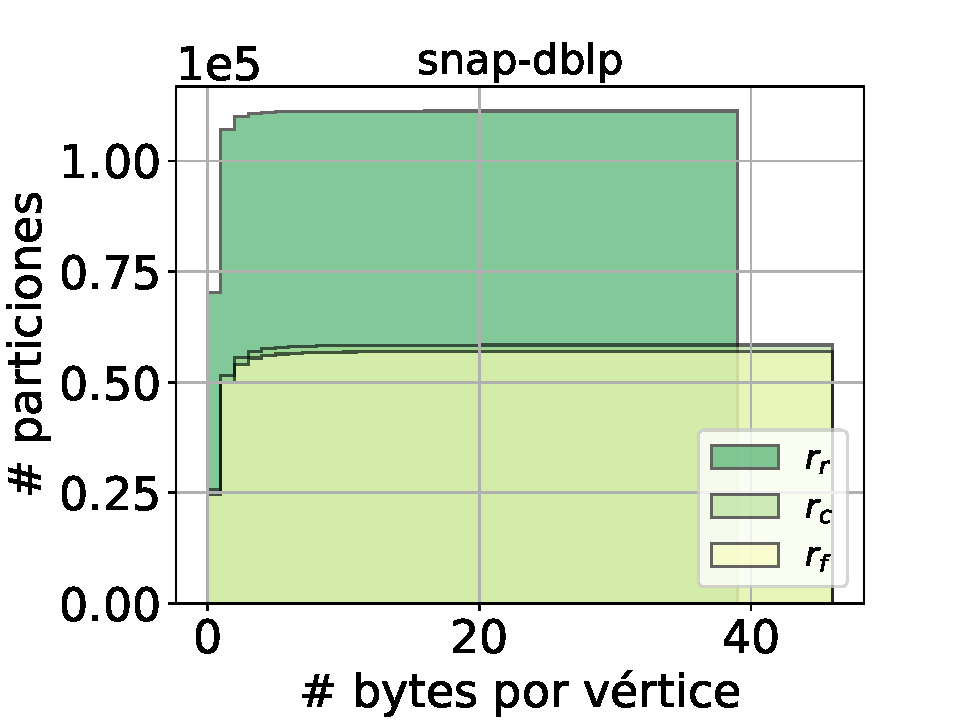
\includegraphics[width=1\linewidth]{../img/cdf/snap-dblp.pdf}
    		\end{minipage}
    		\begin{minipage}{0.45\textwidth}
    			\centering
    			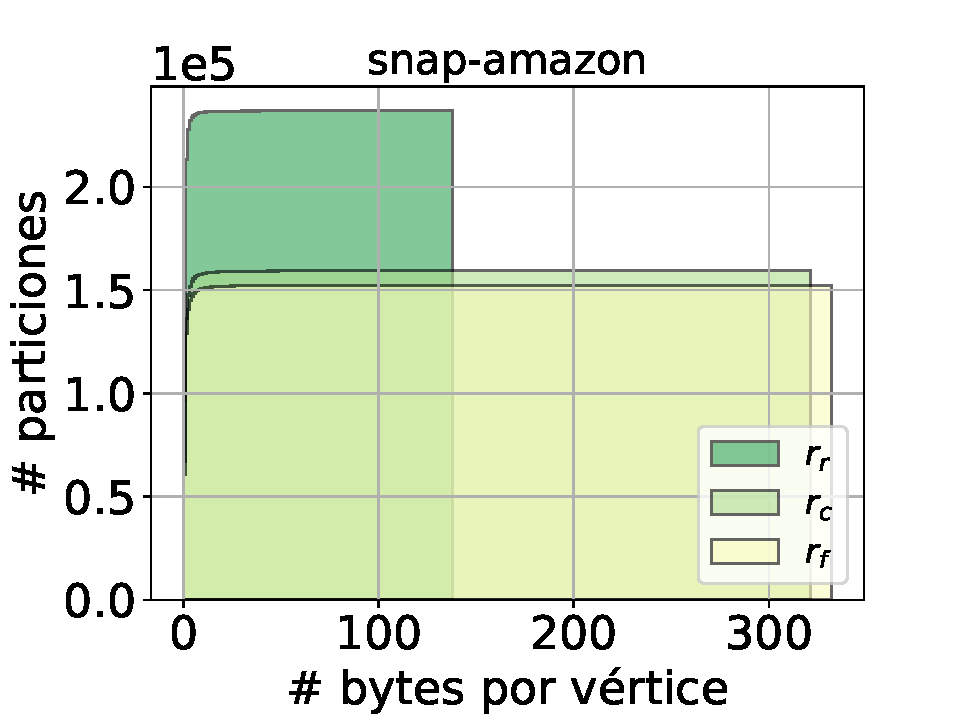
\includegraphics[width=1\linewidth]{../img/cdf/snap-amazon.pdf}
    		\end{minipage}  		
    	\end{minipage}
    	
    	\begin{minipage}{1\textwidth}
    		\centering
    		\begin{minipage}{0.45\textwidth}
    			\centering
    			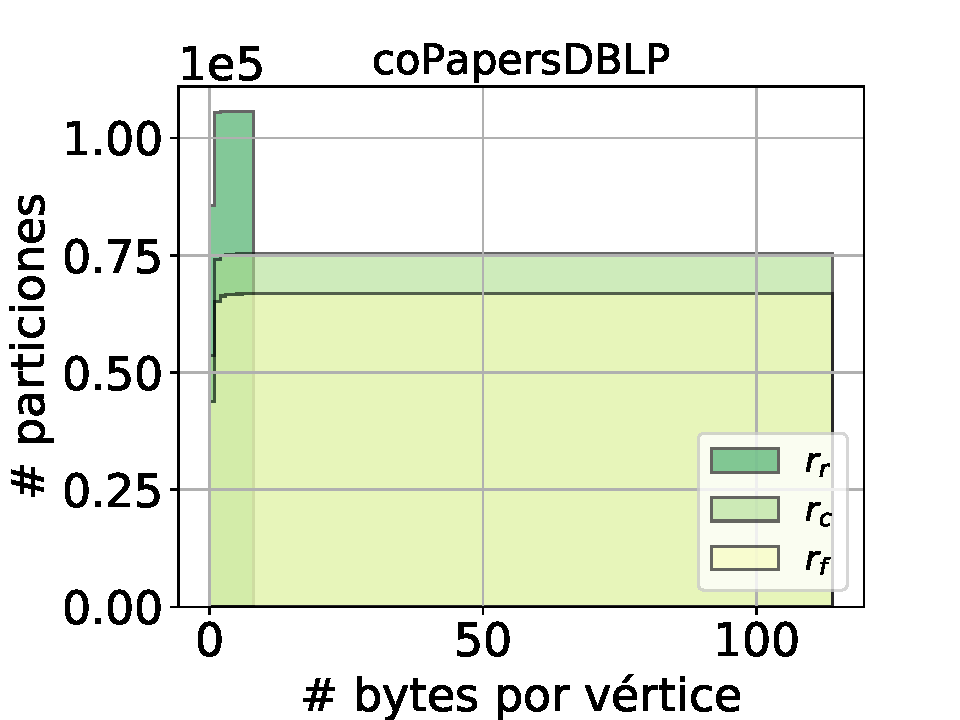
\includegraphics[width=1\linewidth]{../img/cdf/coPapersDBLP.pdf}
    		\end{minipage}
    		\begin{minipage}{0.45\textwidth}
    			\centering
    			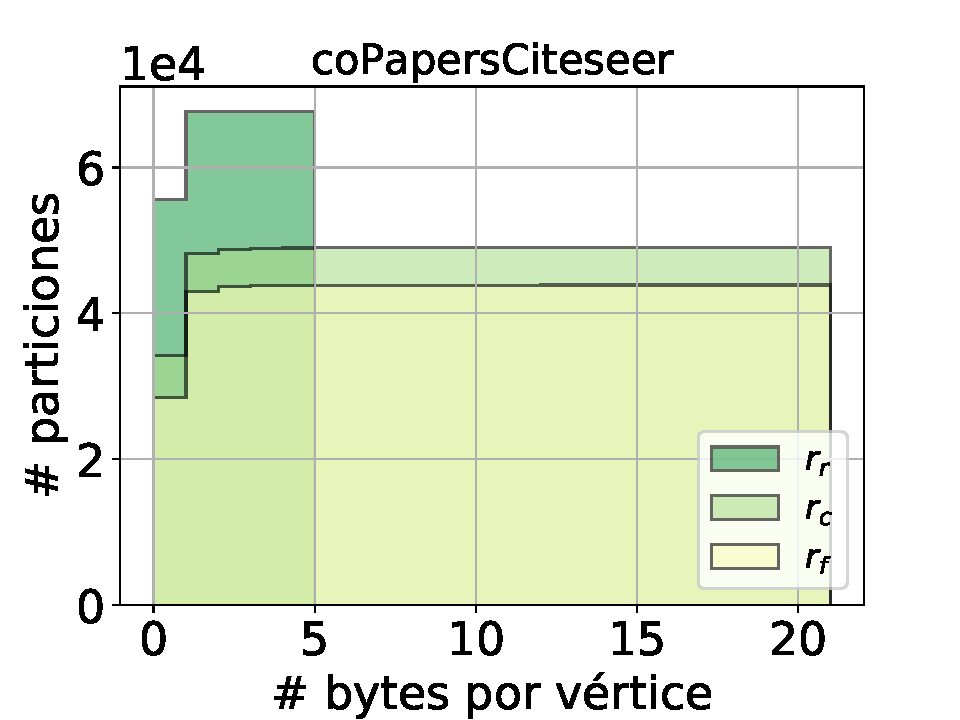
\includegraphics[width=1\linewidth]{../img/cdf/coPapersCiteseer.pdf}
    		\end{minipage}  
    	\end{minipage}	

    \caption{CDF para bytes por vértice en estructuras compactas para cada función de ranking (2).}
\end{figure}

\end{frame}



\begin{frame}
\frametitle{Resultados - Estructura compacta}

\begin{figure}
	\centering
	
    	\begin{minipage}{1\textwidth}
    		\centering
    		\begin{minipage}{0.8\textwidth}
    			\centering
    			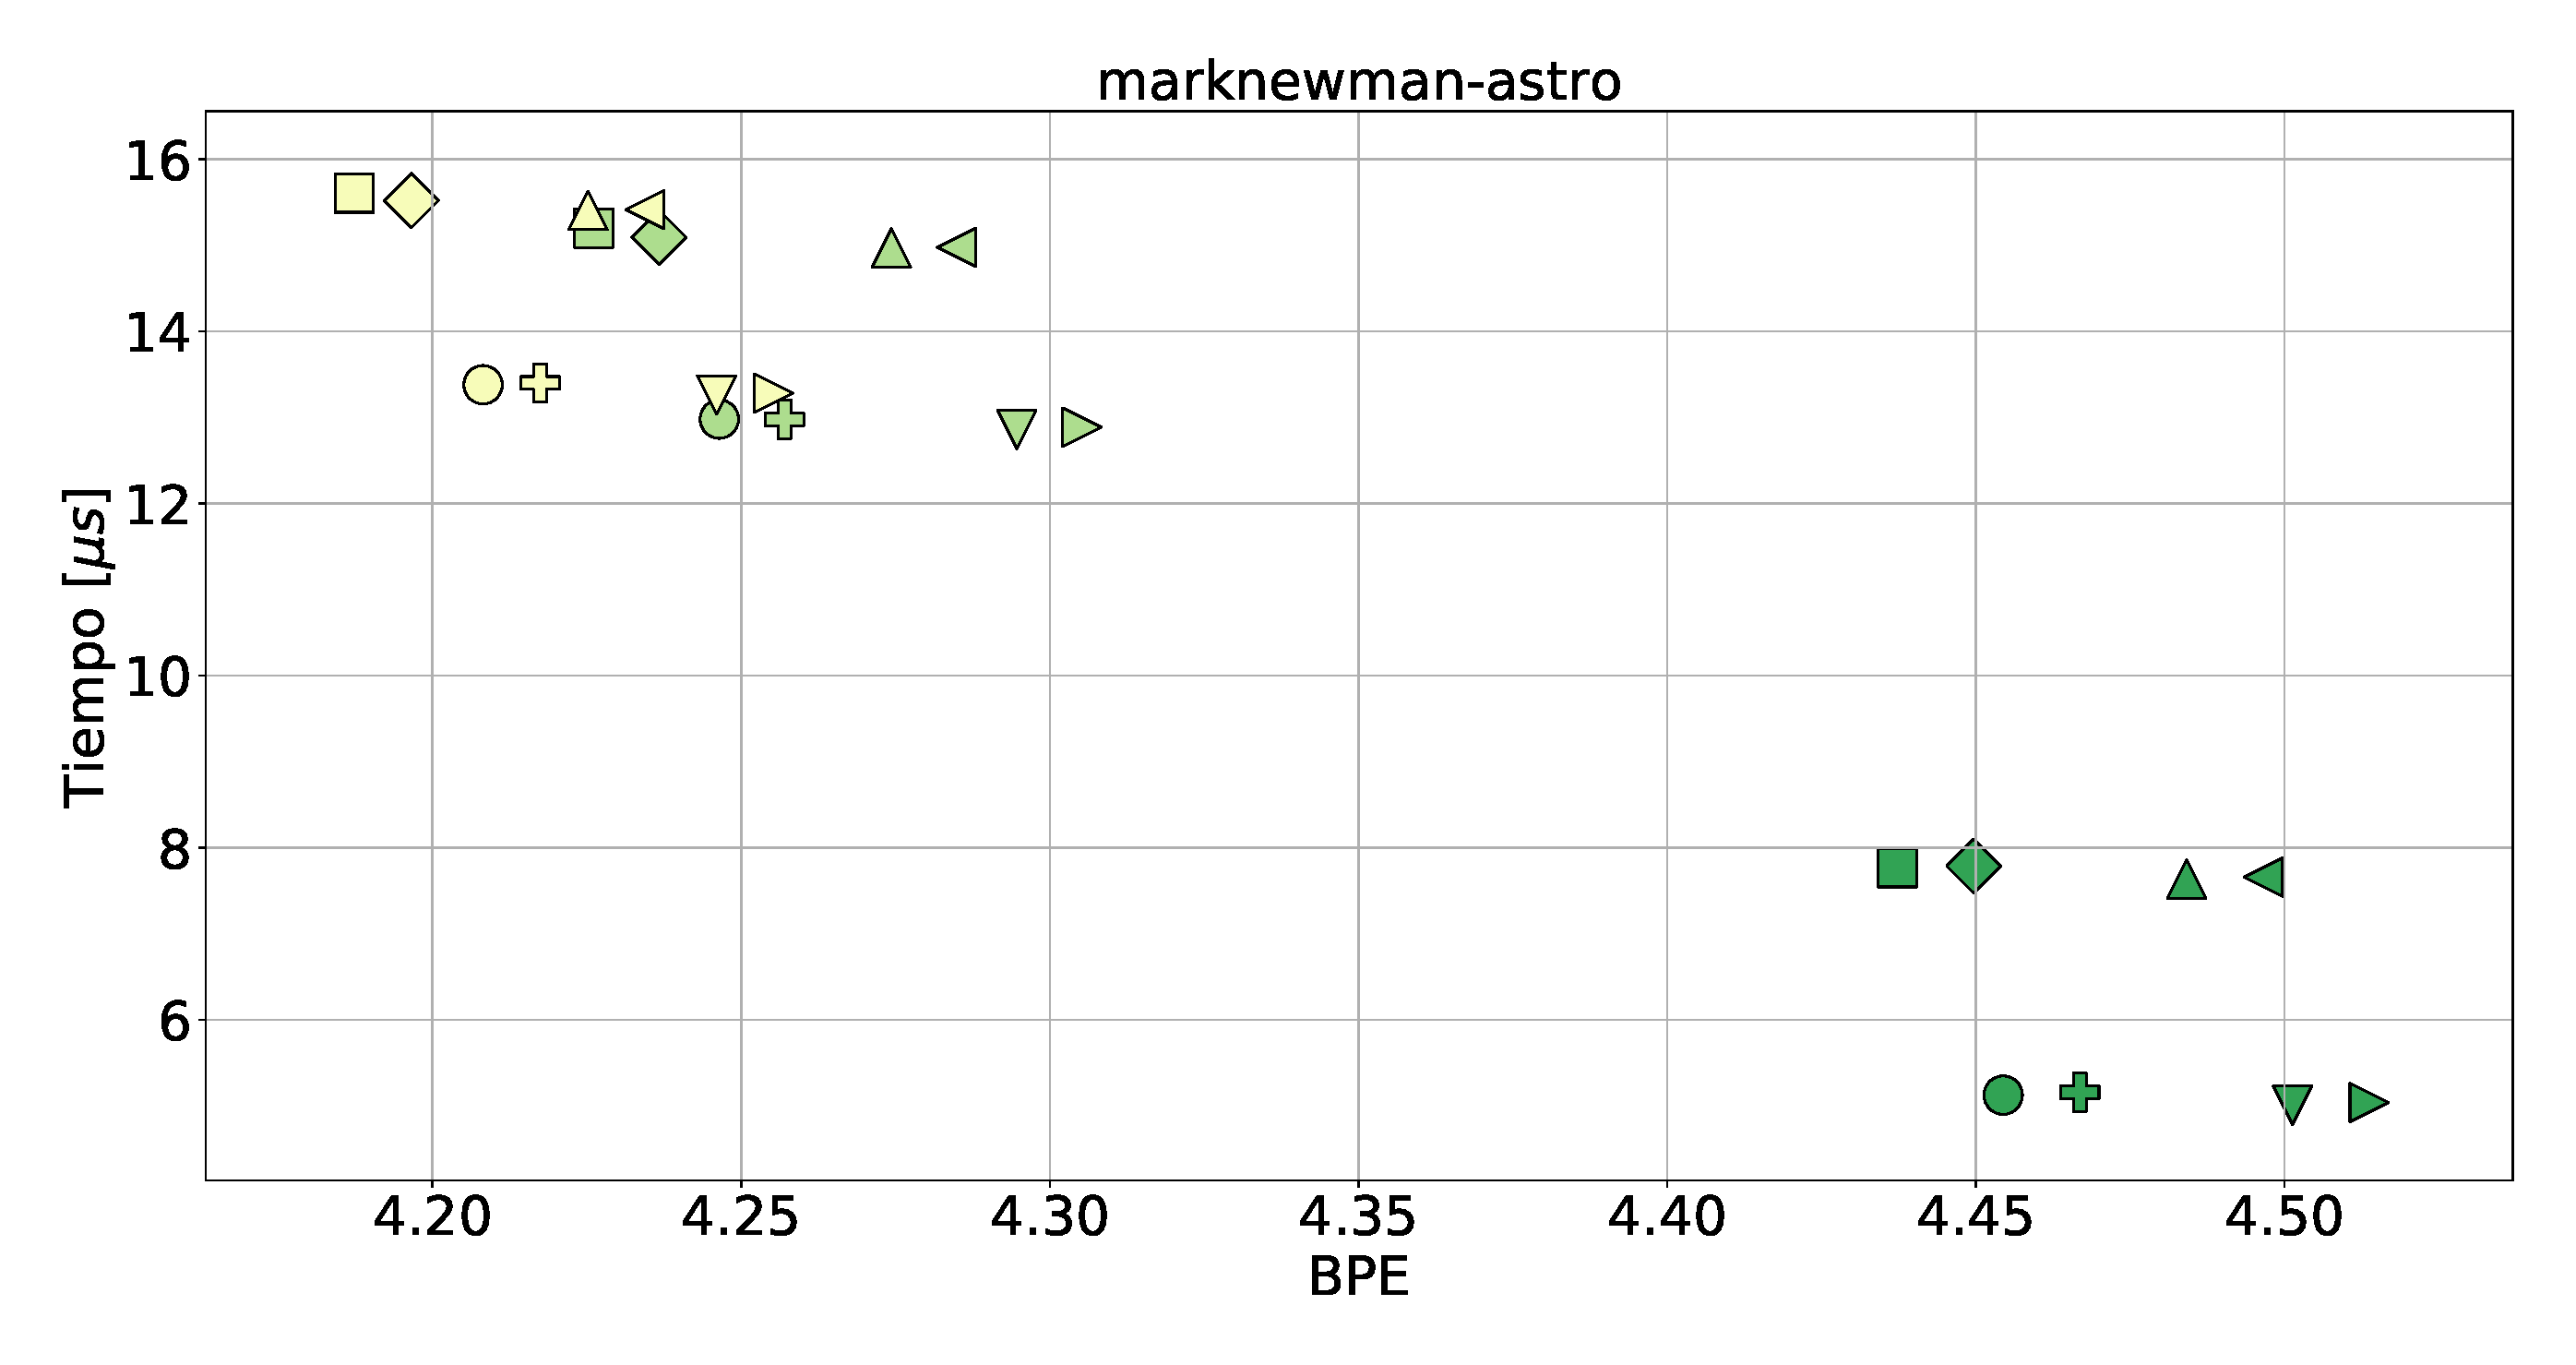
\includegraphics[width=1\linewidth]{../img/sdsl/aleatorioBig/marknewman-astro.pdf}
    		\end{minipage}
    		\begin{minipage}{0.15\textwidth}
    			\centering
    			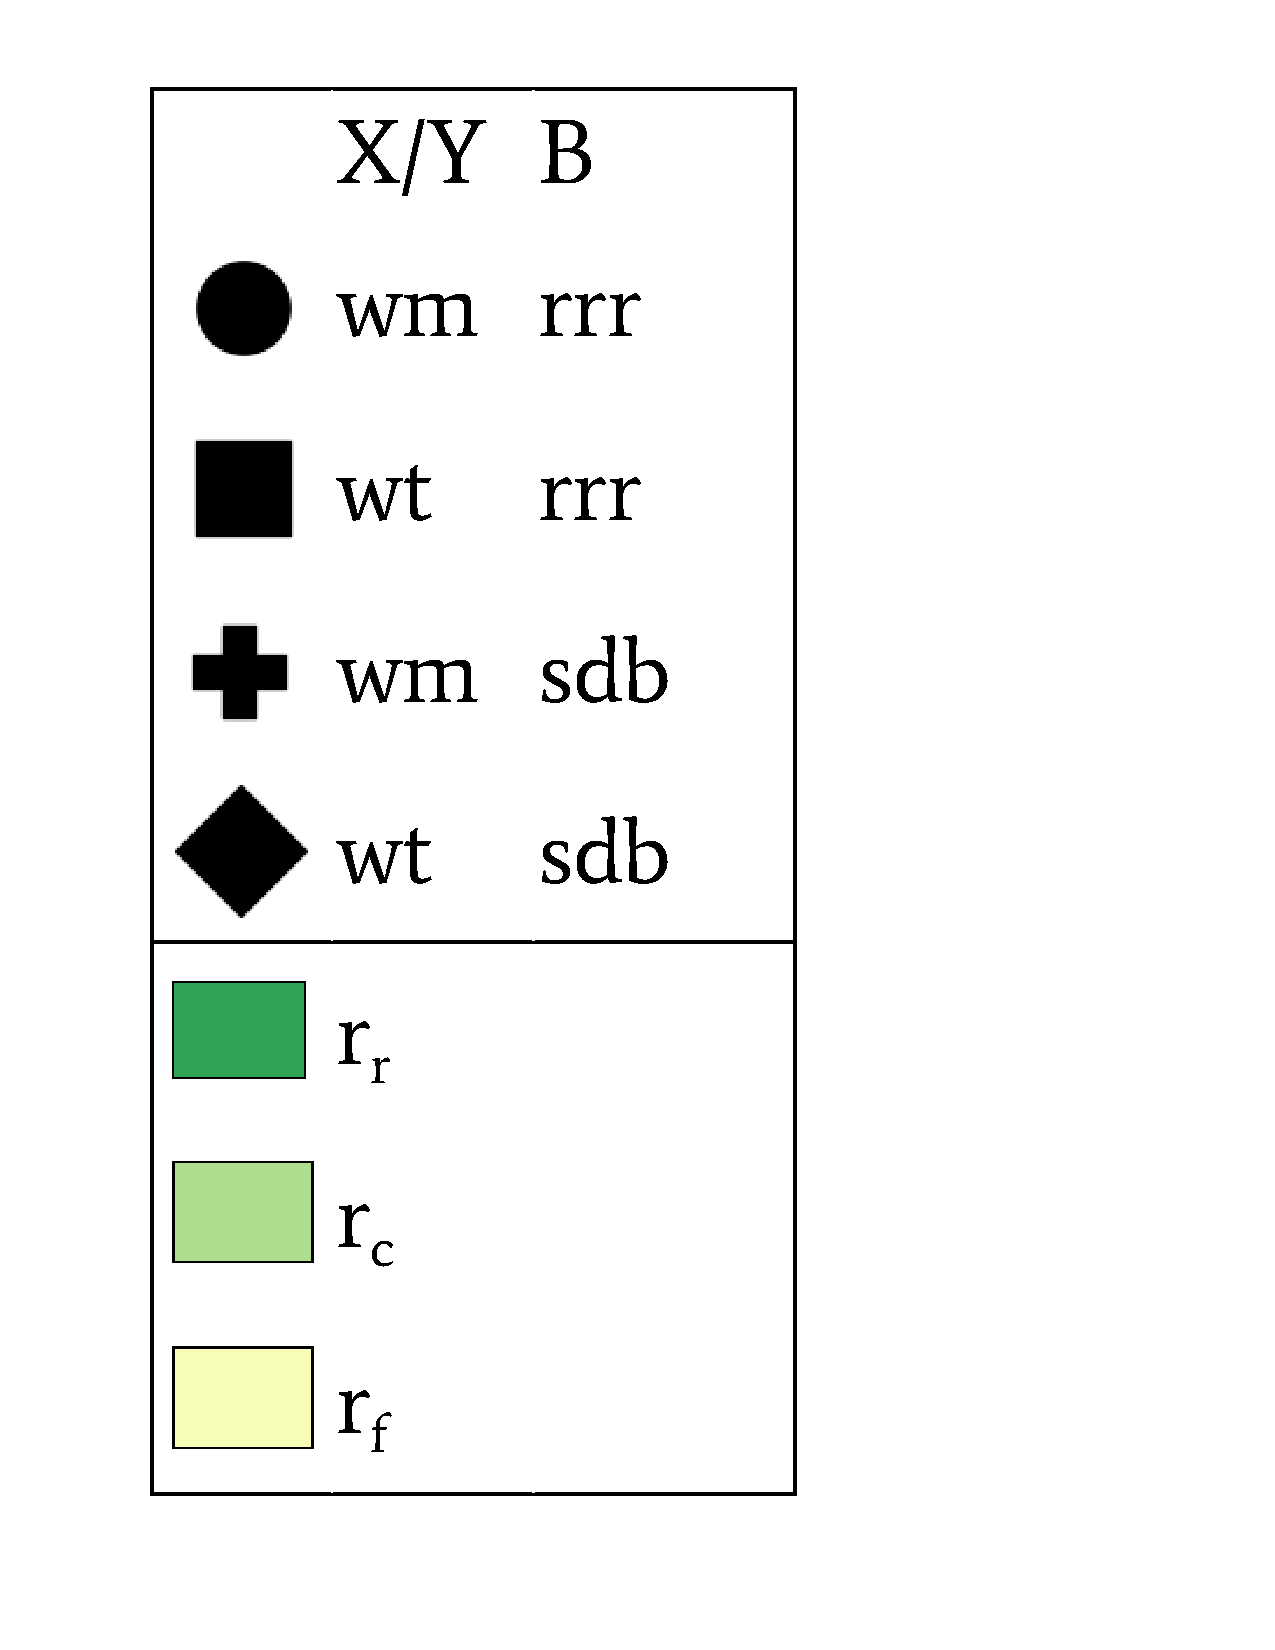
\includegraphics[scale=.15, clip, trim=70 0 0 0]{../img/sdsl/label.pdf}
    		\end{minipage}	
    	\end{minipage}

	\caption{BPE y Tiempo de acceso aleatorio medio para posibles estructuras compactas, por cada función de ranking, para marknewman-astro.}
\end{figure}

\end{frame}

\begin{frame}
\frametitle{Resultados - Estructura compacta}

\begin{figure}
	\centering
	
    	\begin{minipage}{1\textwidth}
    		\centering
    		\begin{minipage}{0.8\textwidth}
    			\centering
    			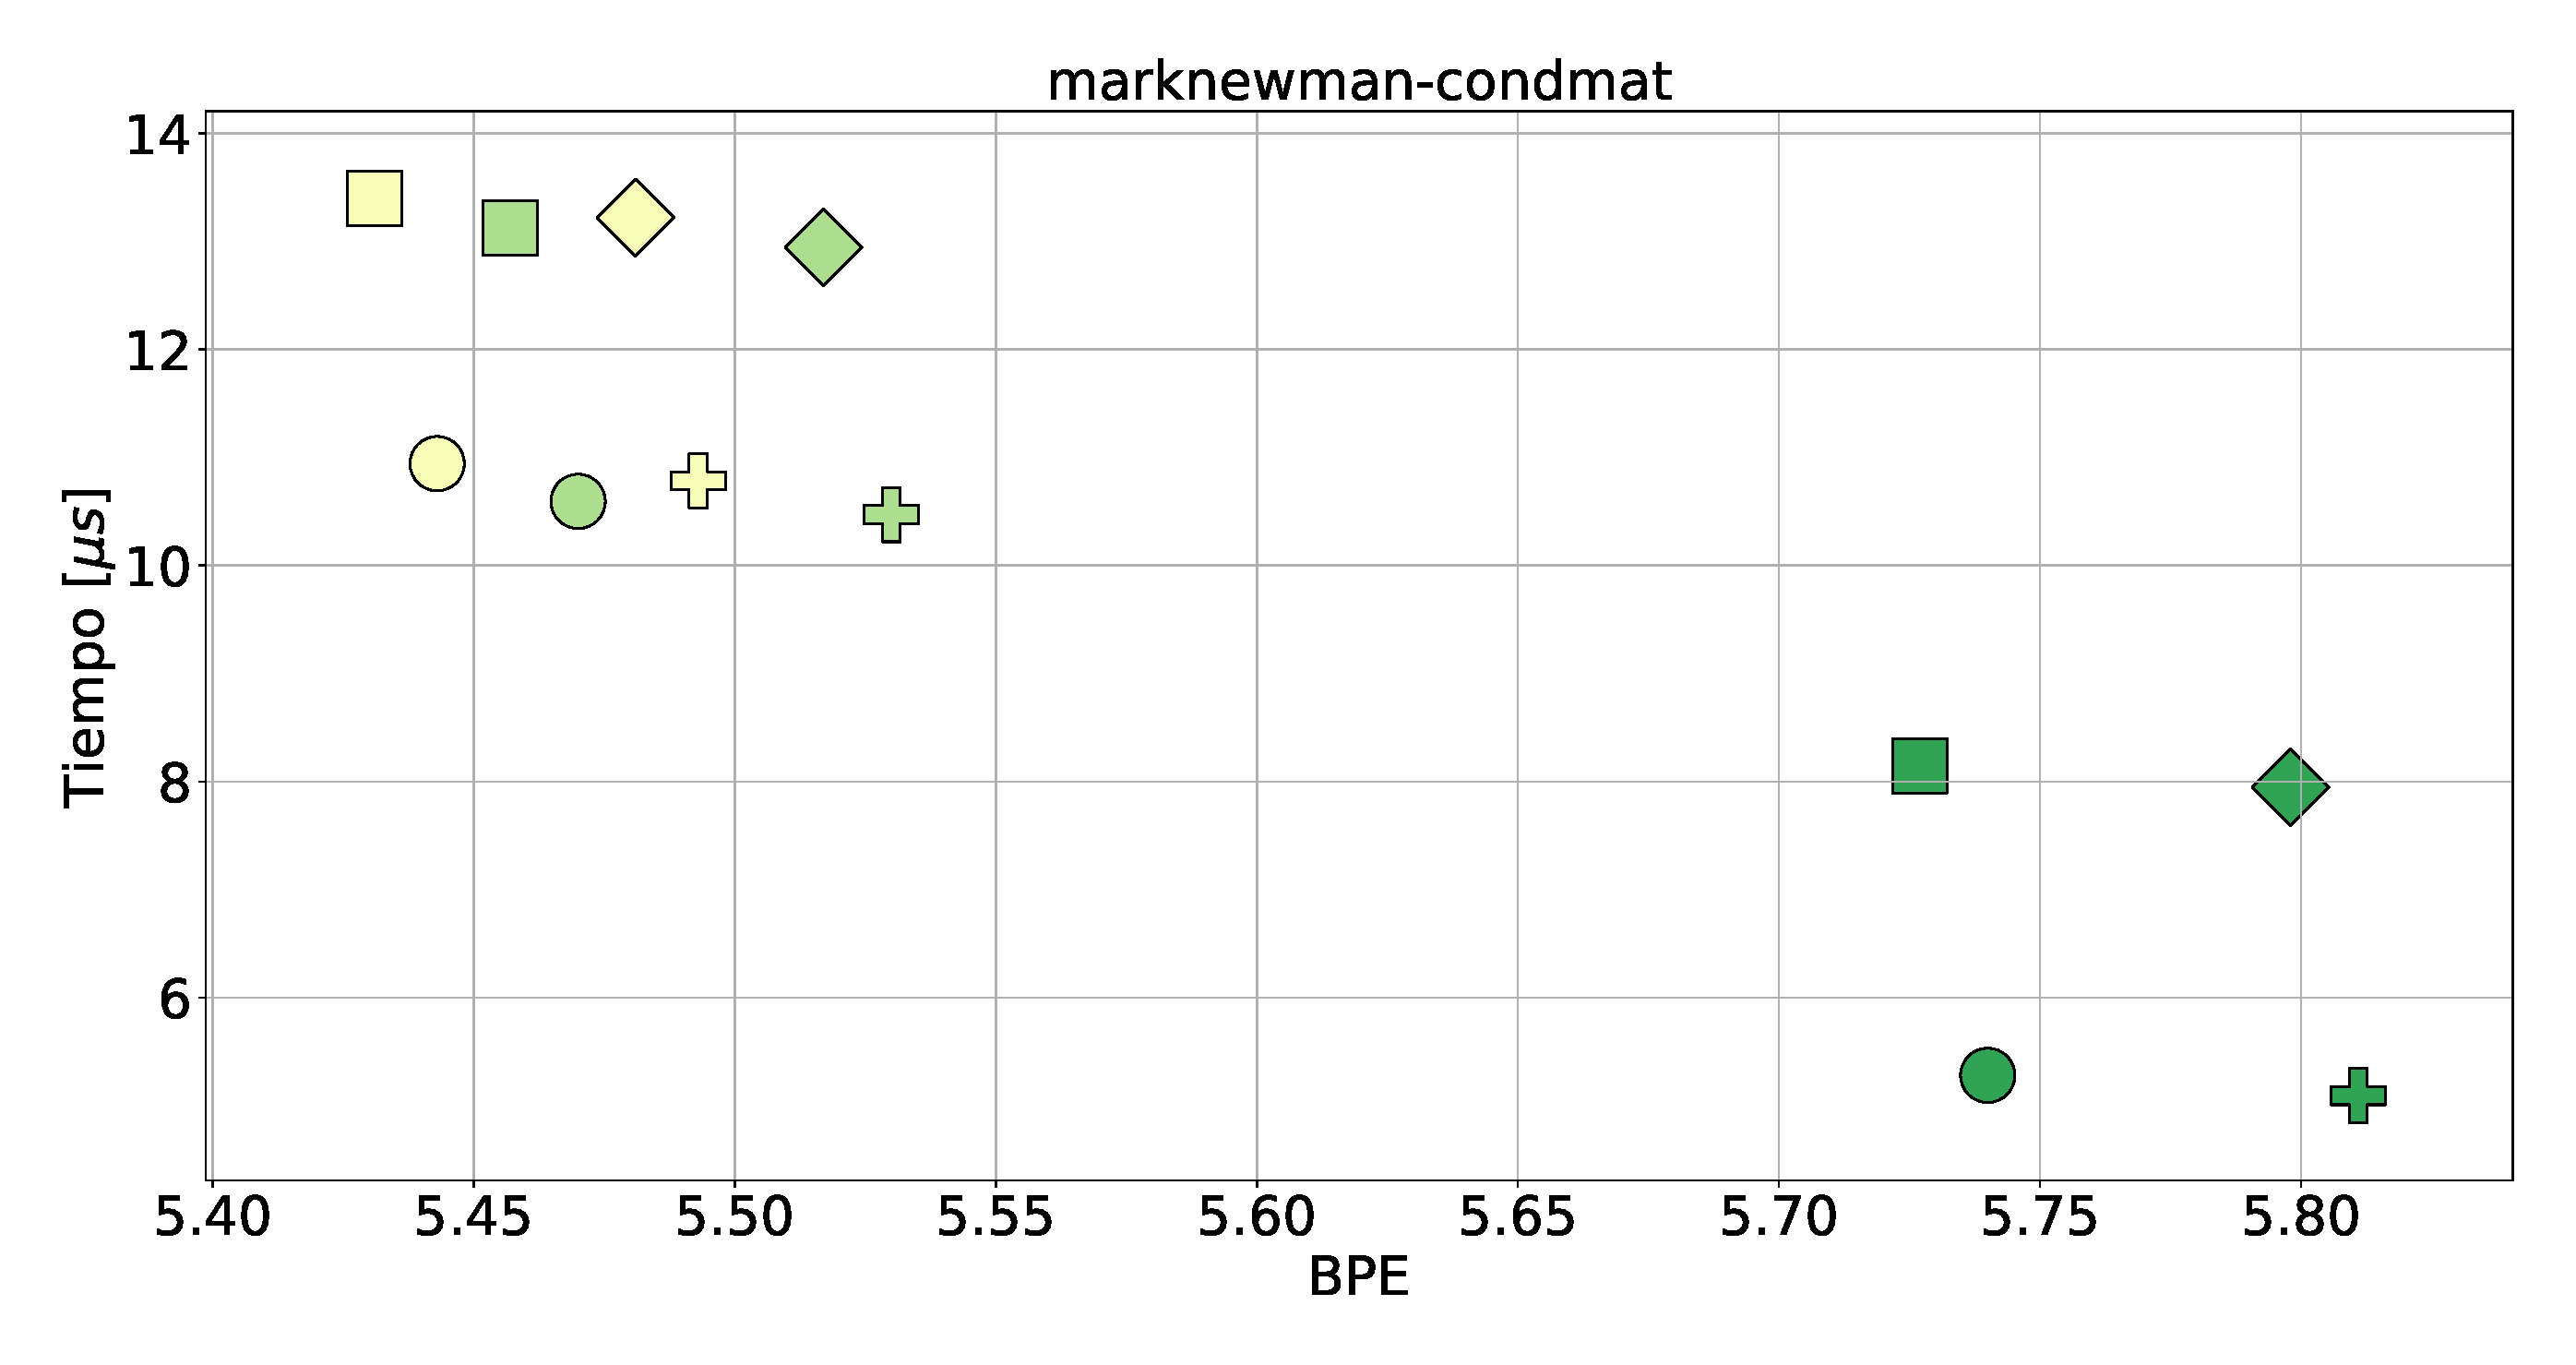
\includegraphics[width=1\linewidth]{../img/sdsl/aleatorioBig/marknewman-condmat.pdf}
    		\end{minipage}
    		\begin{minipage}{0.15\textwidth}
    			\centering
    			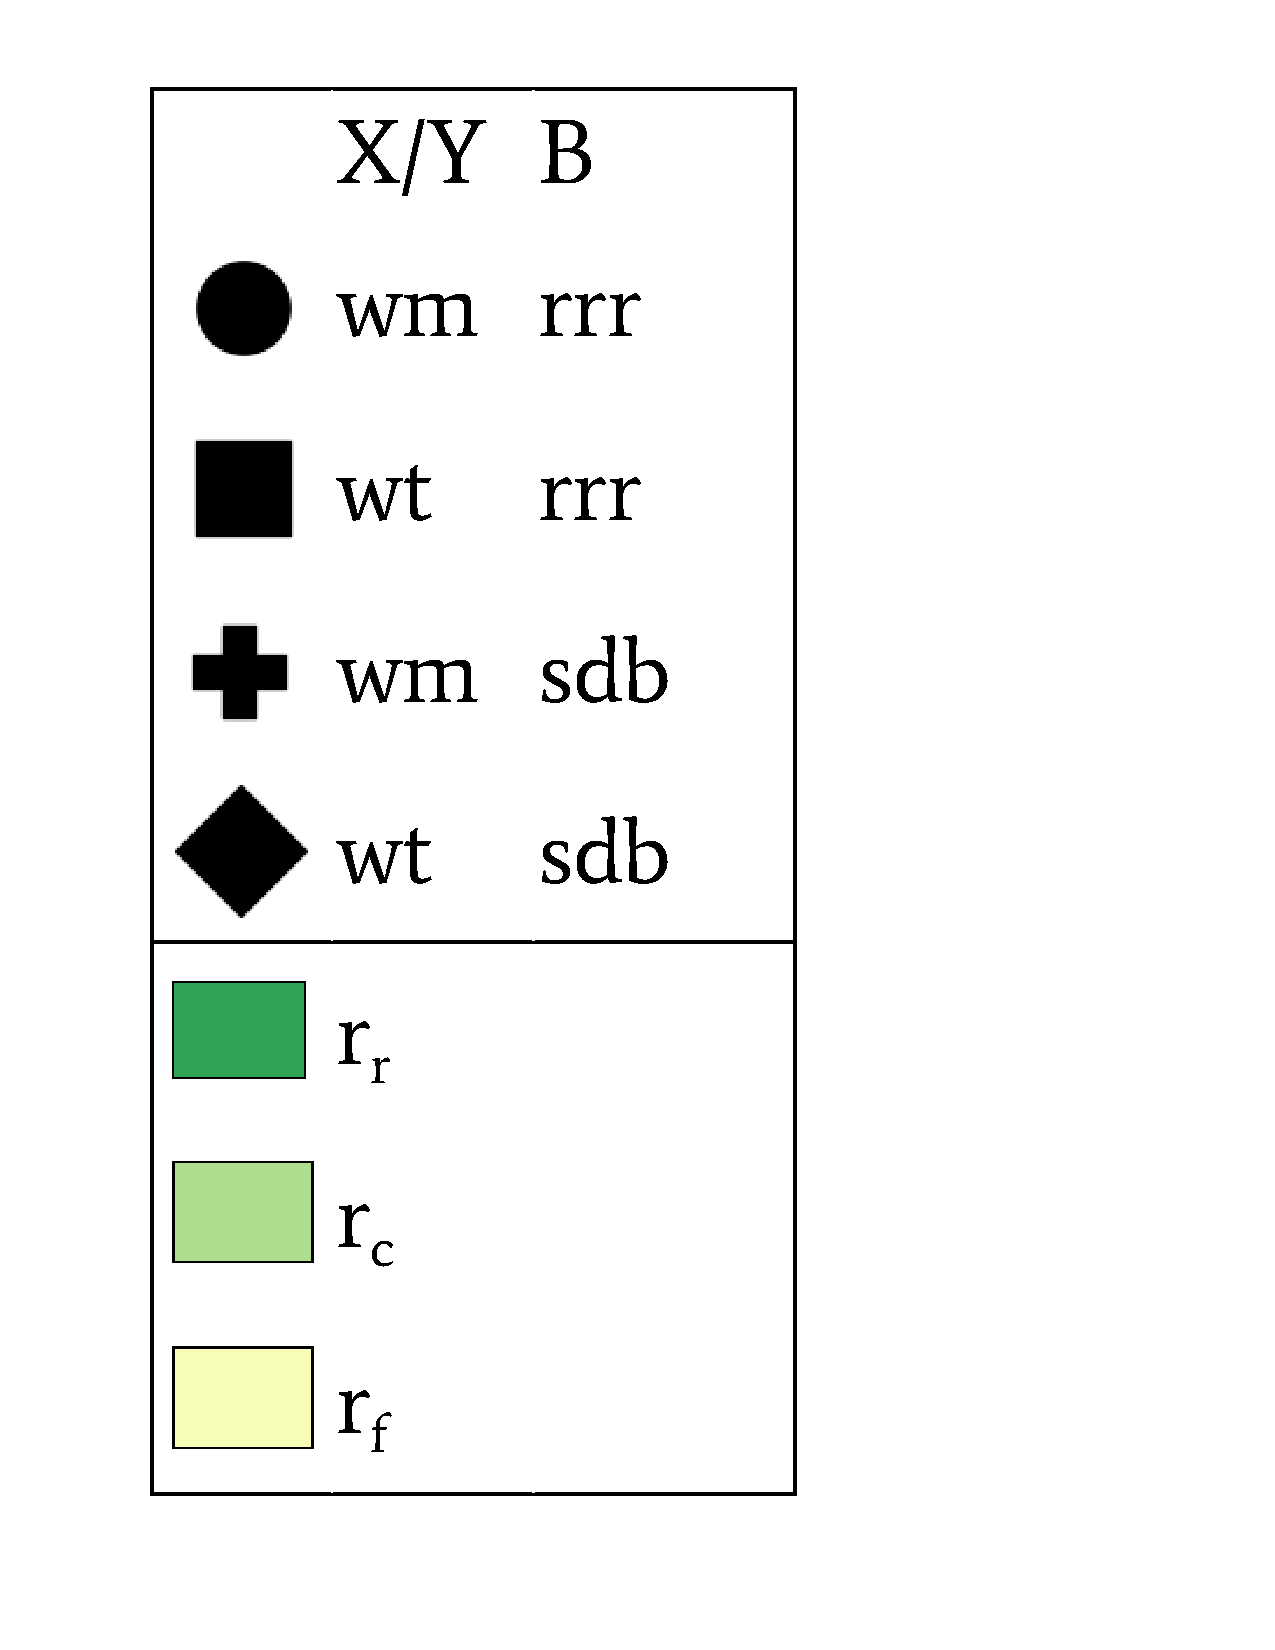
\includegraphics[scale=.15, clip, trim=70 0 0 0]{../img/sdsl/label.pdf}
    		\end{minipage}	
    	\end{minipage}

	\caption{BPE y Tiempo de acceso aleatorio medio para posibles estructuras compactas, por cada función de ranking, para marknewman-condmat.}
\end{figure}

\end{frame}

\begin{frame}
\frametitle{Resultados - Estructura compacta}

\begin{figure}
	\centering
	
    	\begin{minipage}{1\textwidth}
    		\centering
    		\begin{minipage}{0.8\textwidth}
    			\centering
    			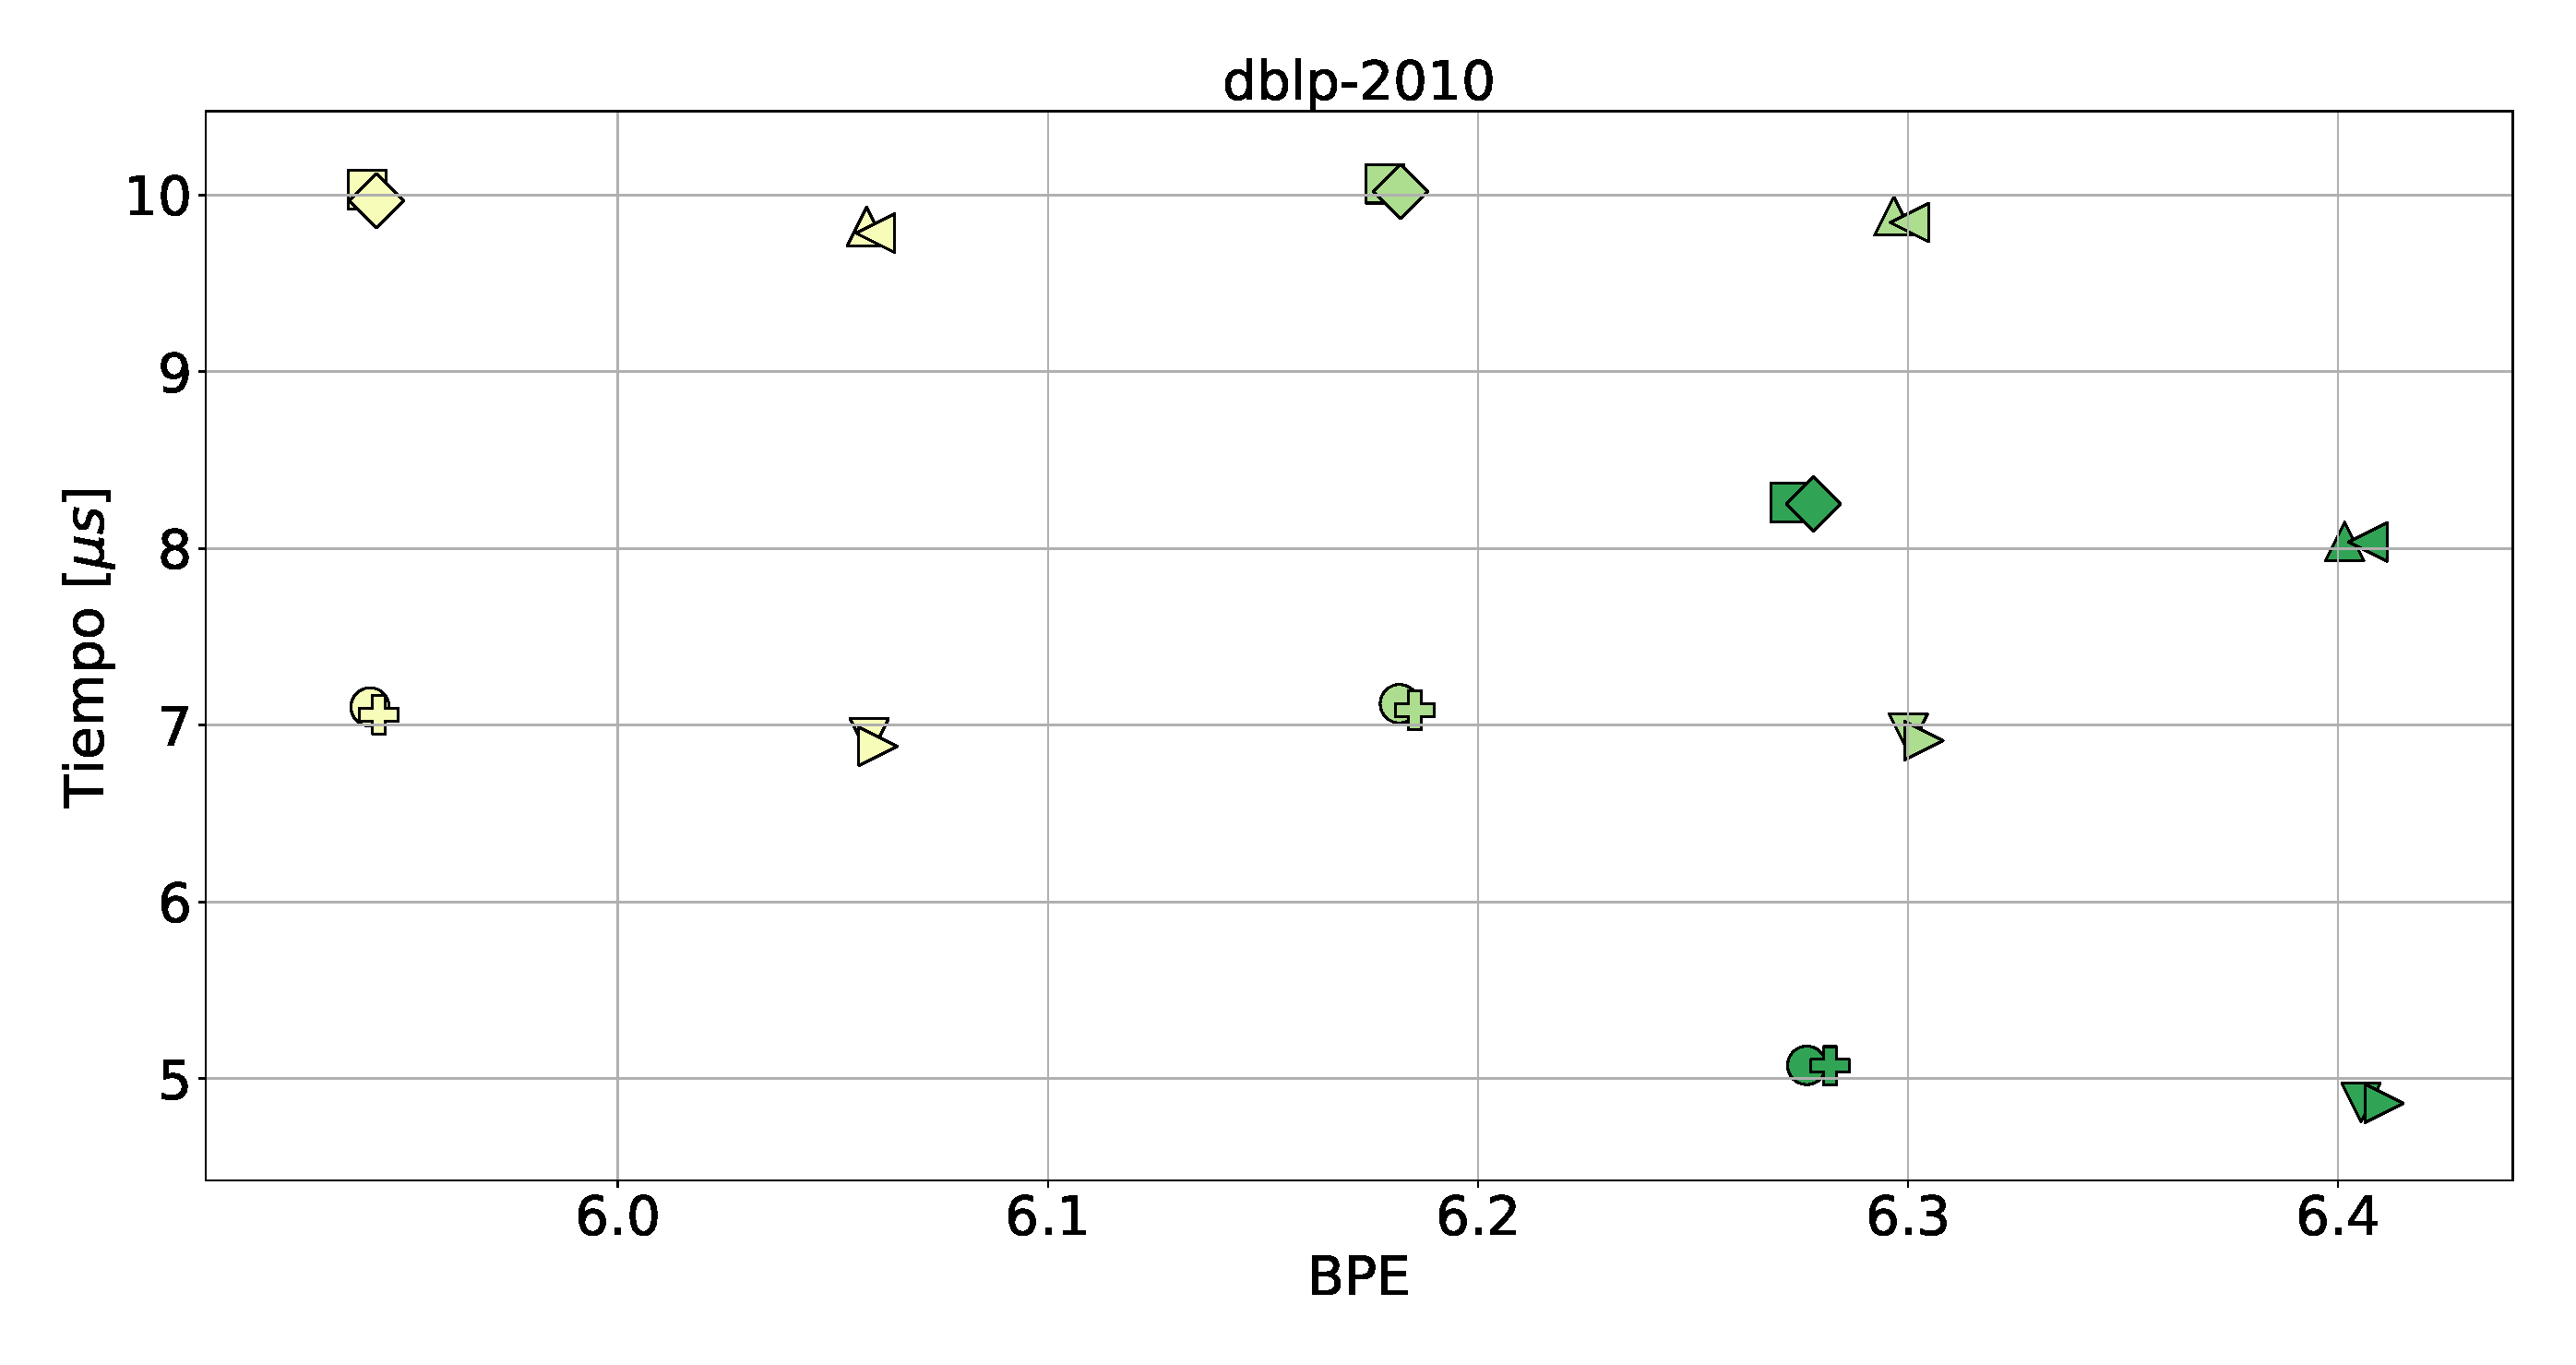
\includegraphics[width=1\linewidth]{../img/sdsl/aleatorioBig/dblp-2010.pdf}
    		\end{minipage}
    		\begin{minipage}{0.15\textwidth}
    			\centering
    			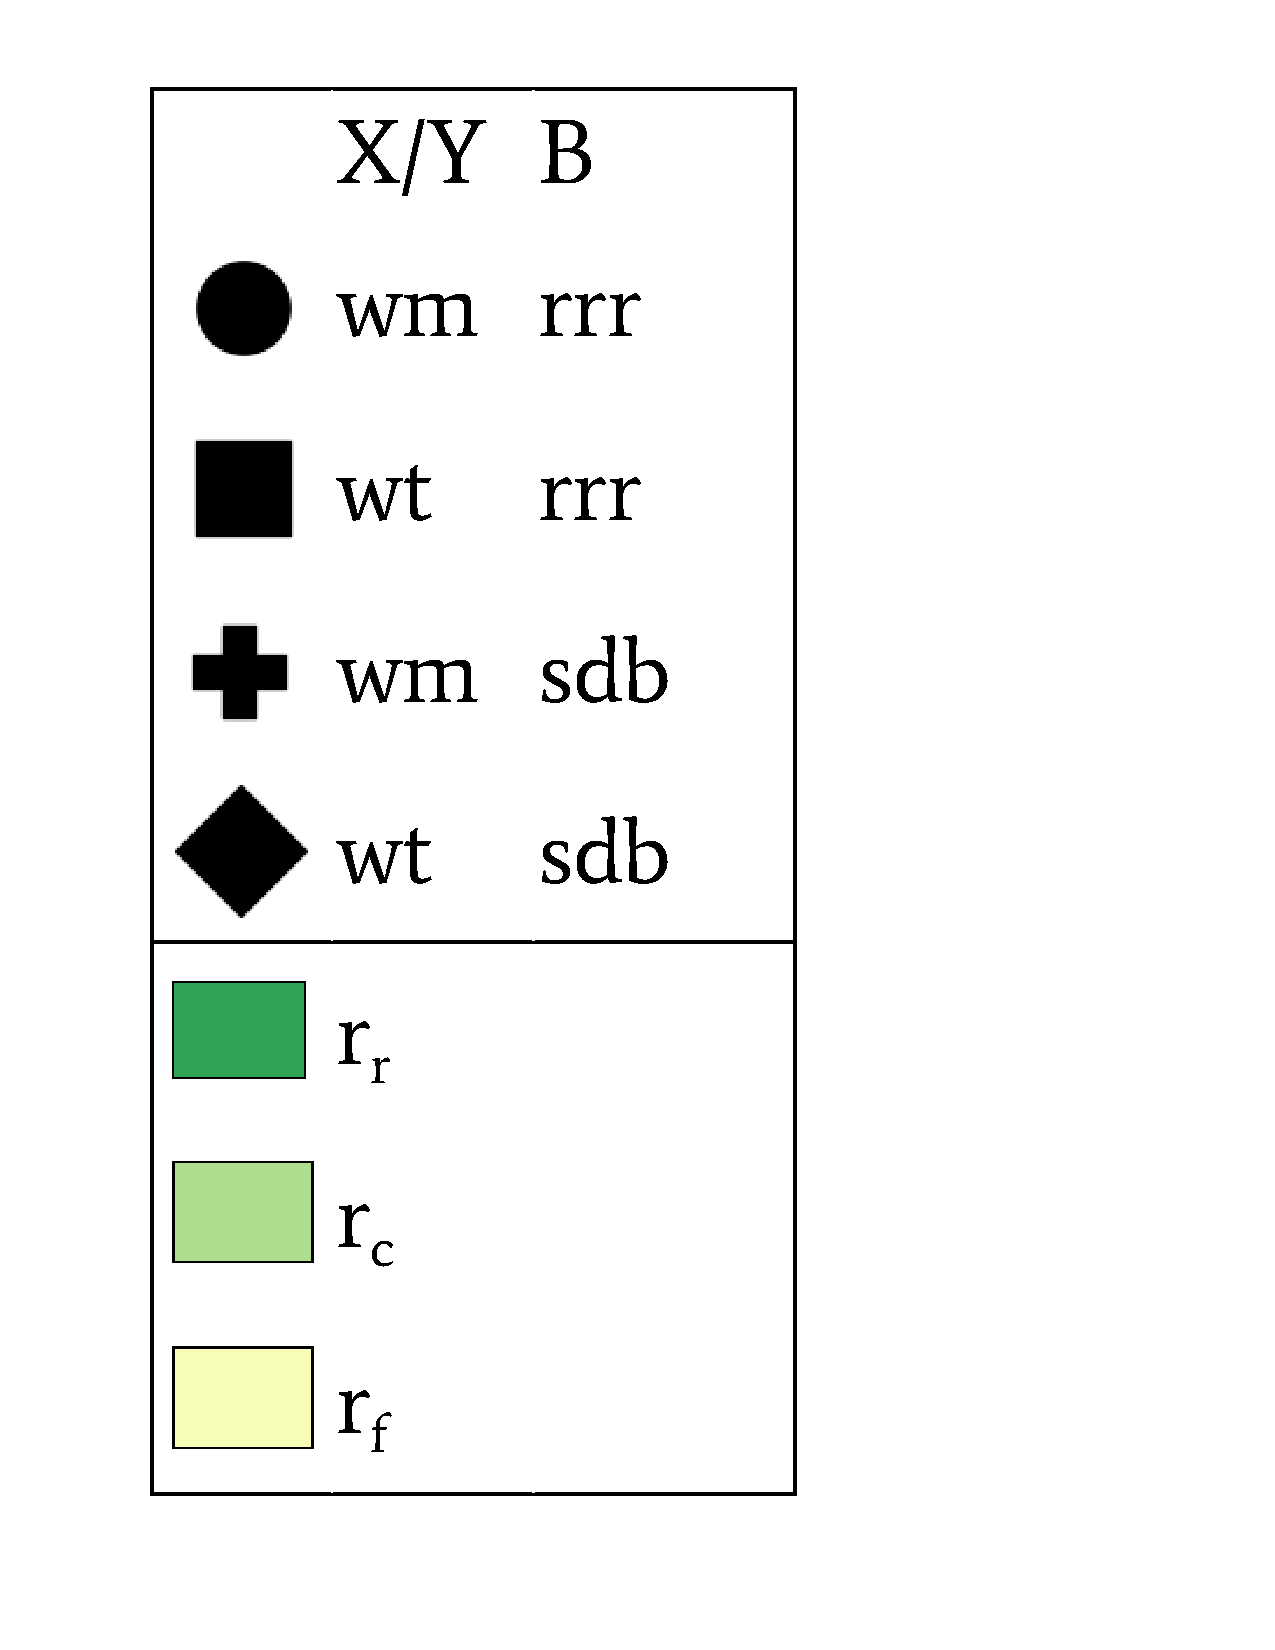
\includegraphics[scale=.15, clip, trim=70 0 0 0]{../img/sdsl/label.pdf}
    		\end{minipage}	
    	\end{minipage}

	\caption{BPE y Tiempo de acceso aleatorio medio para posibles estructuras compactas, por cada función de ranking, para dblp-2010.}
\end{figure}

\end{frame}

\begin{frame}
\frametitle{Resultados - Estructura compacta}

\begin{figure}
	\centering
	
    	\begin{minipage}{1\textwidth}
    		\centering
    		\begin{minipage}{0.8\textwidth}
    			\centering
    			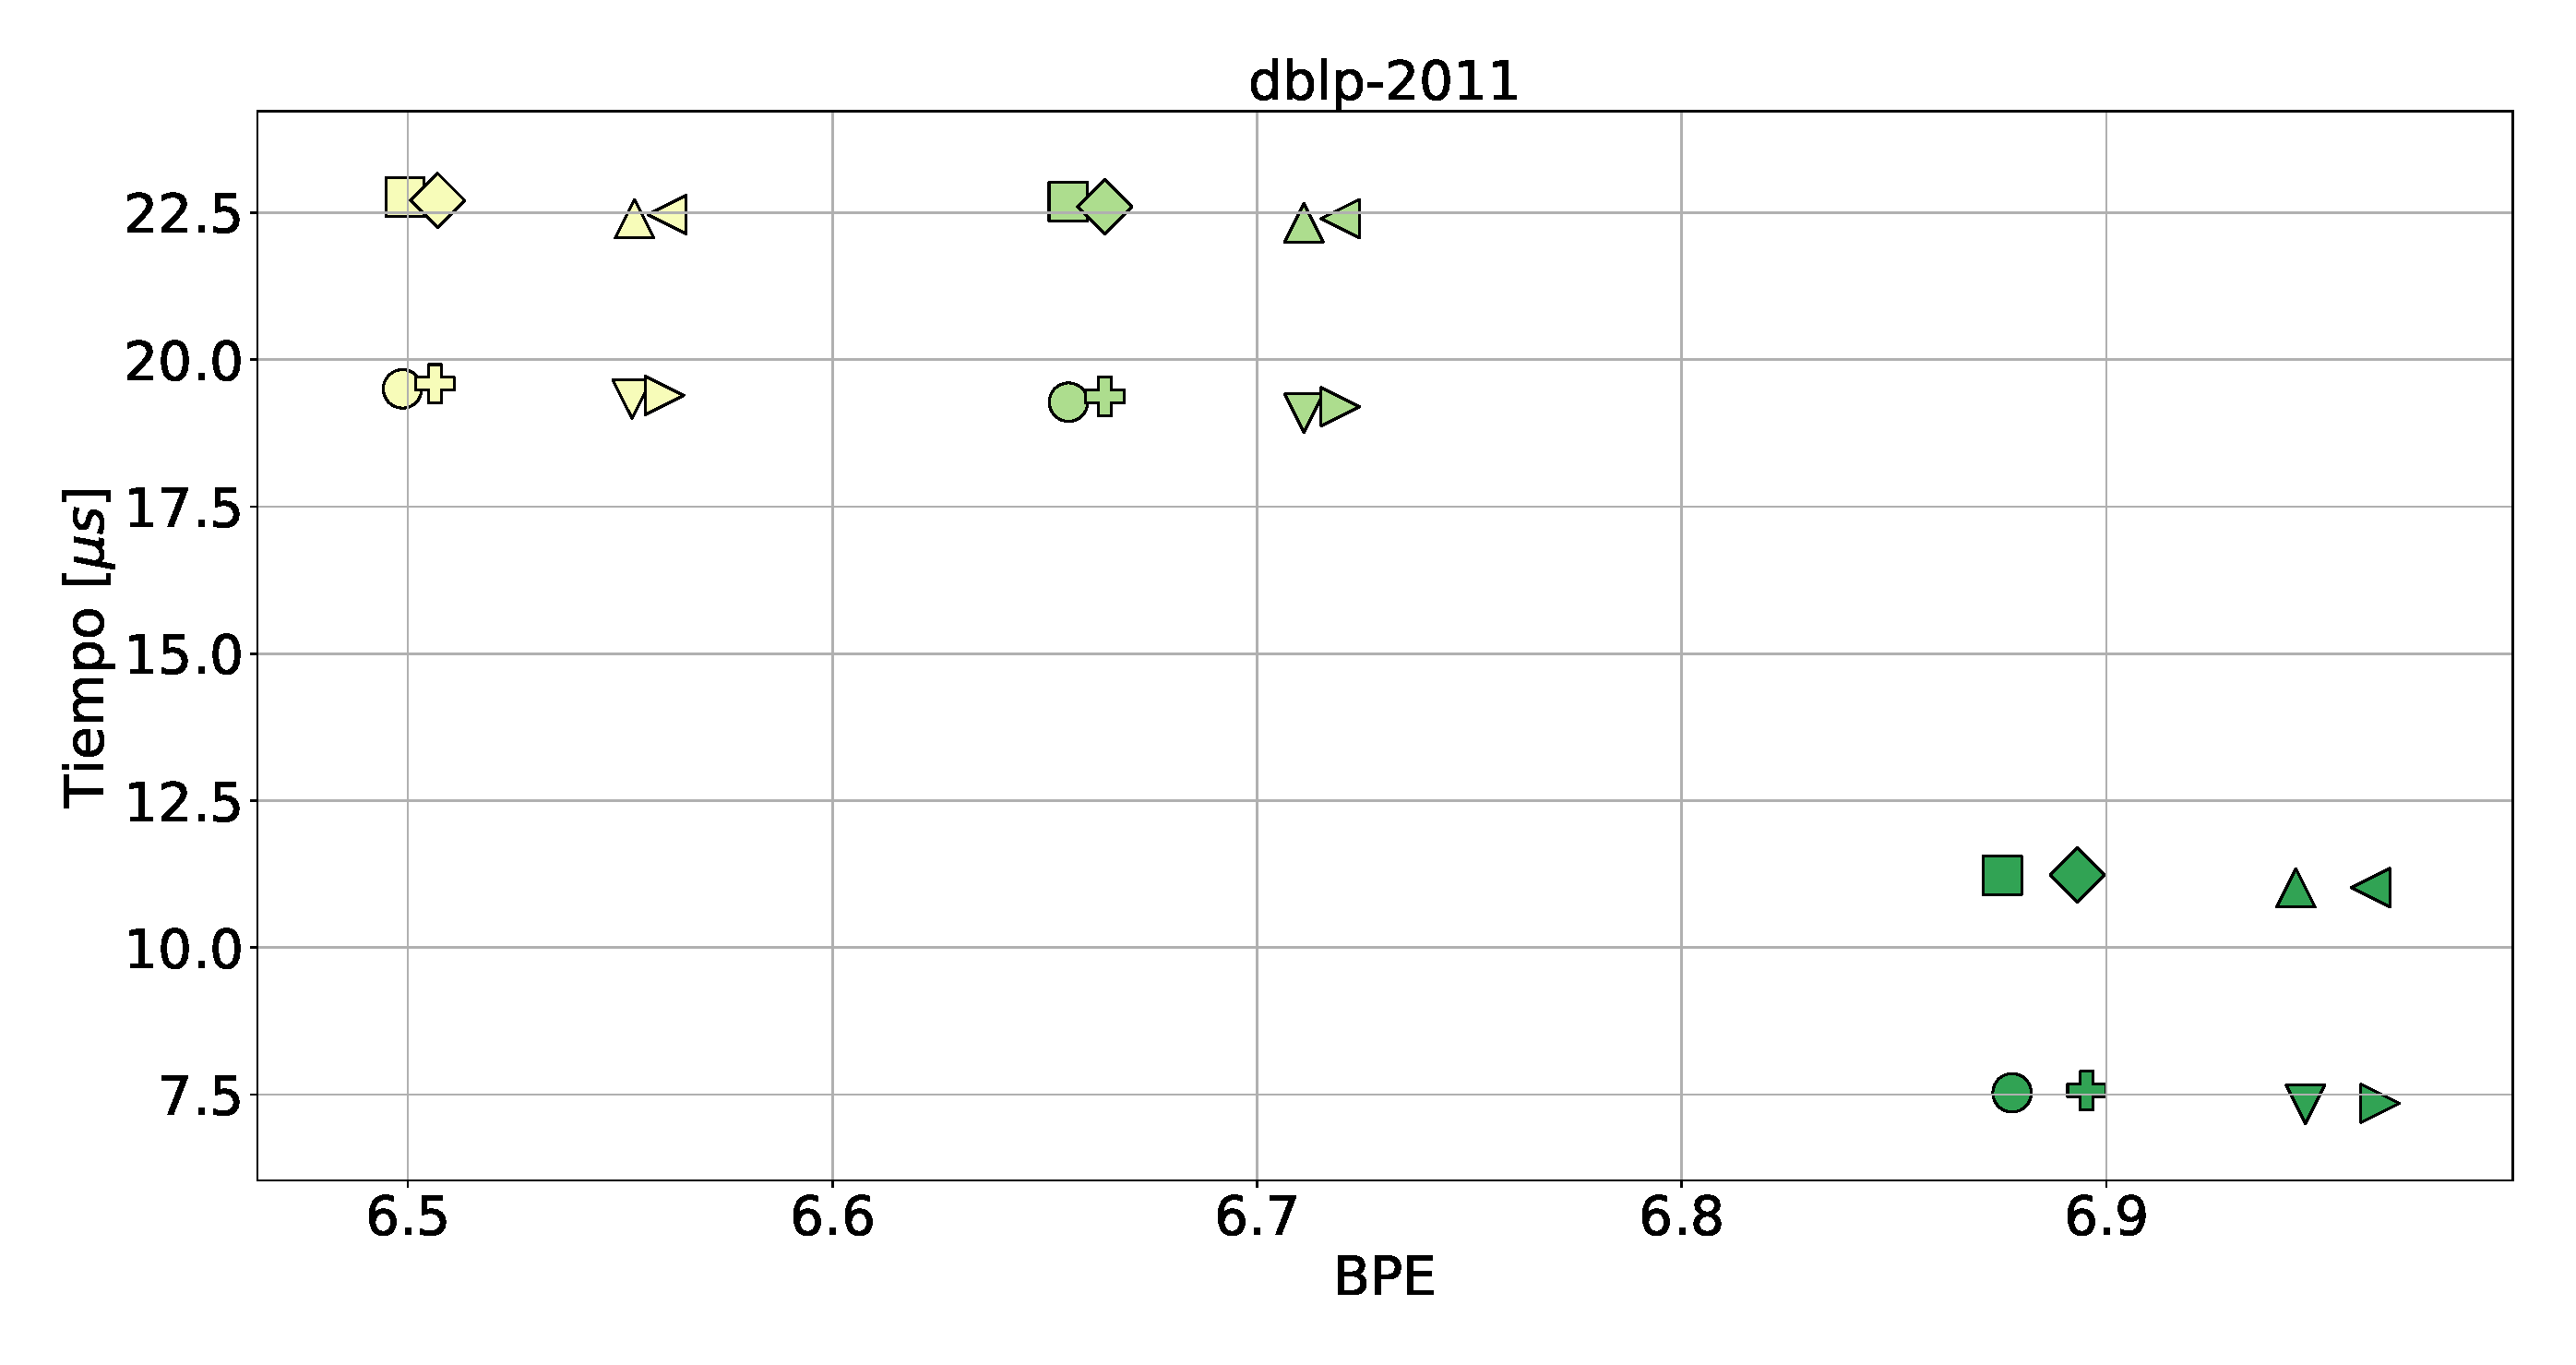
\includegraphics[width=1\linewidth]{../img/sdsl/aleatorioBig/dblp-2011.pdf}
    		\end{minipage}
    		\begin{minipage}{0.15\textwidth}
    			\centering
    			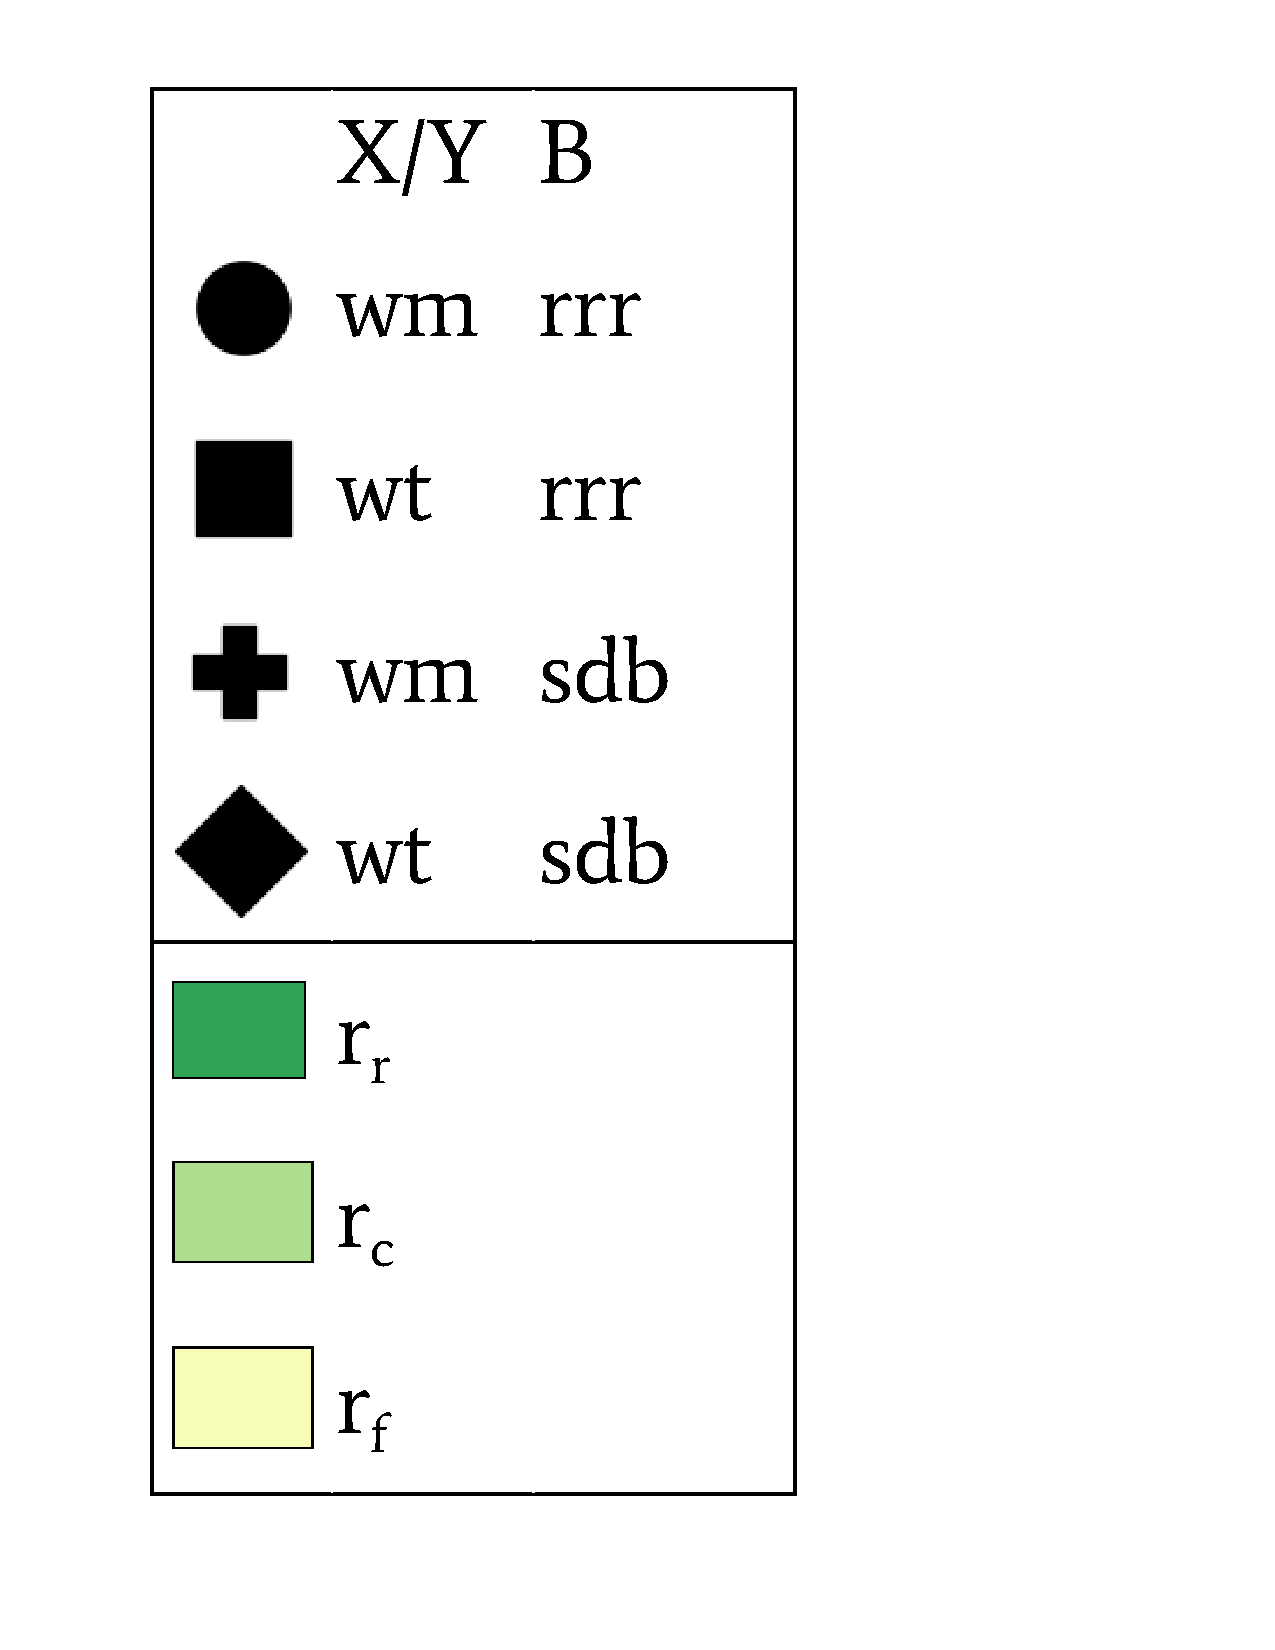
\includegraphics[scale=.15, clip, trim=70 0 0 0]{../img/sdsl/label.pdf}
    		\end{minipage}	
    	\end{minipage}

	\caption{BPE y Tiempo de acceso aleatorio medio para posibles estructuras compactas, por cada función de ranking, para dblp-2011.}
\end{figure}

\end{frame}

\begin{frame}
\frametitle{Resultados - Estructura compacta}

\begin{figure}
	\centering
	
    	\begin{minipage}{1\textwidth}
    		\centering
    		\begin{minipage}{0.8\textwidth}
    			\centering
    			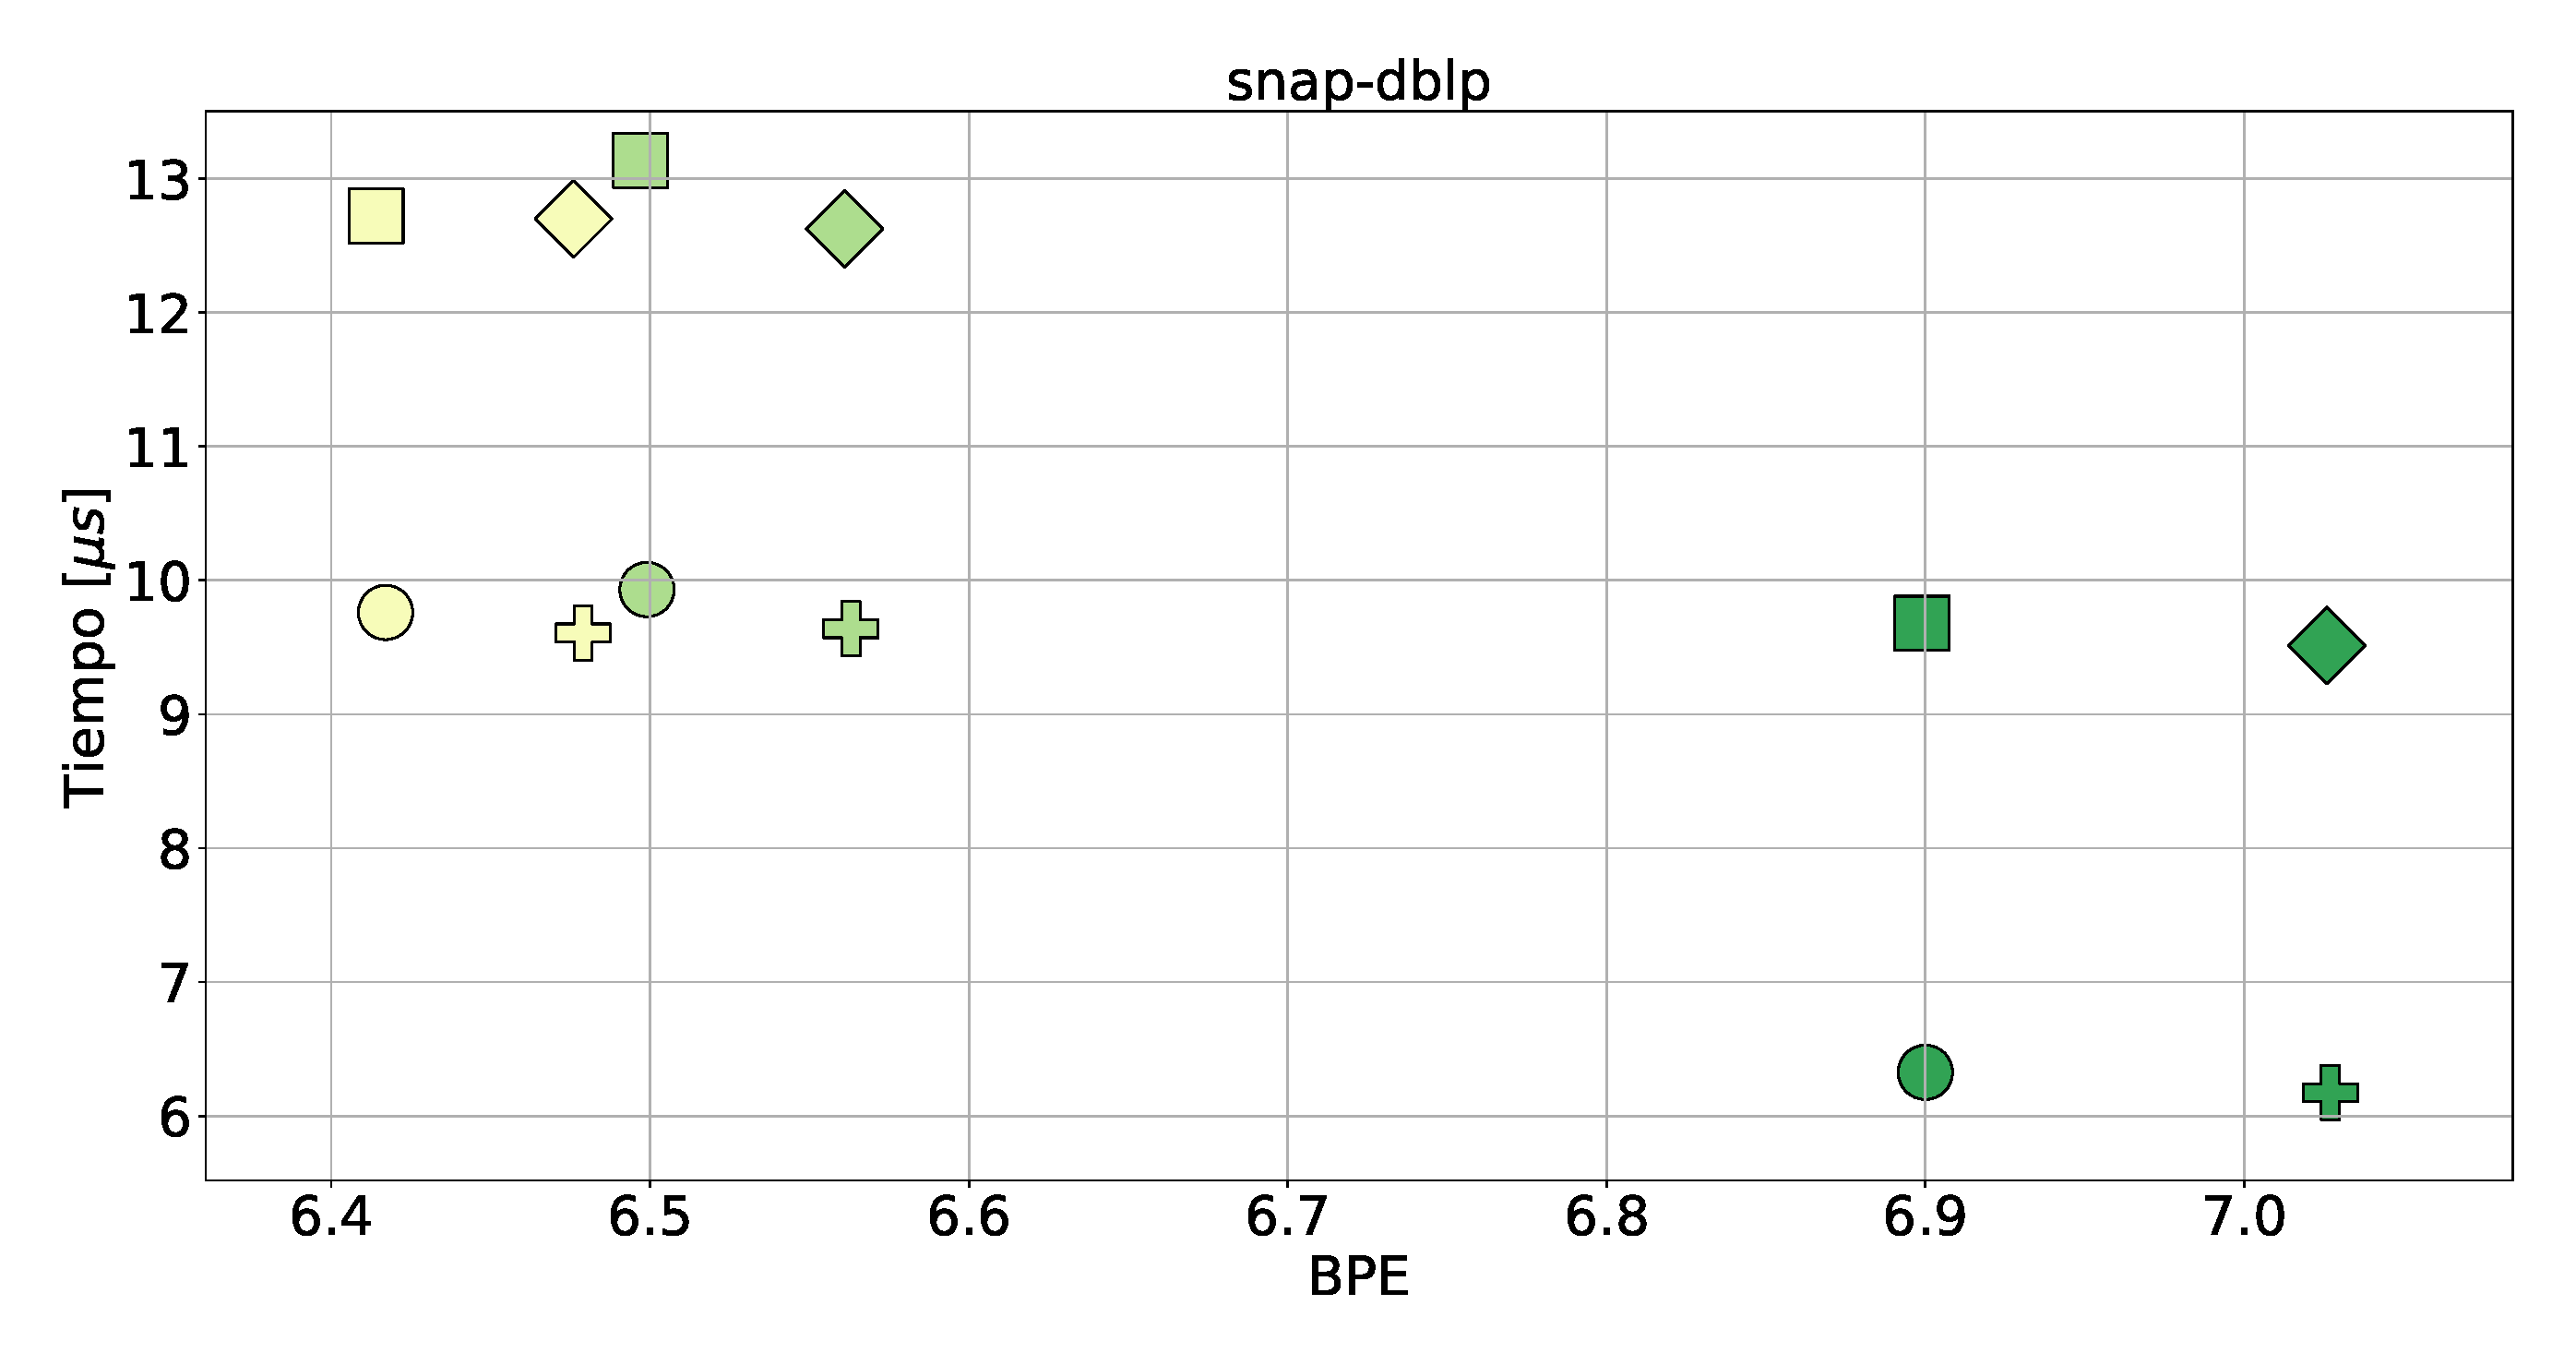
\includegraphics[width=1\linewidth]{../img/sdsl/aleatorioBig/snap-dblp.pdf}
    		\end{minipage}
    		\begin{minipage}{0.15\textwidth}
    			\centering
    			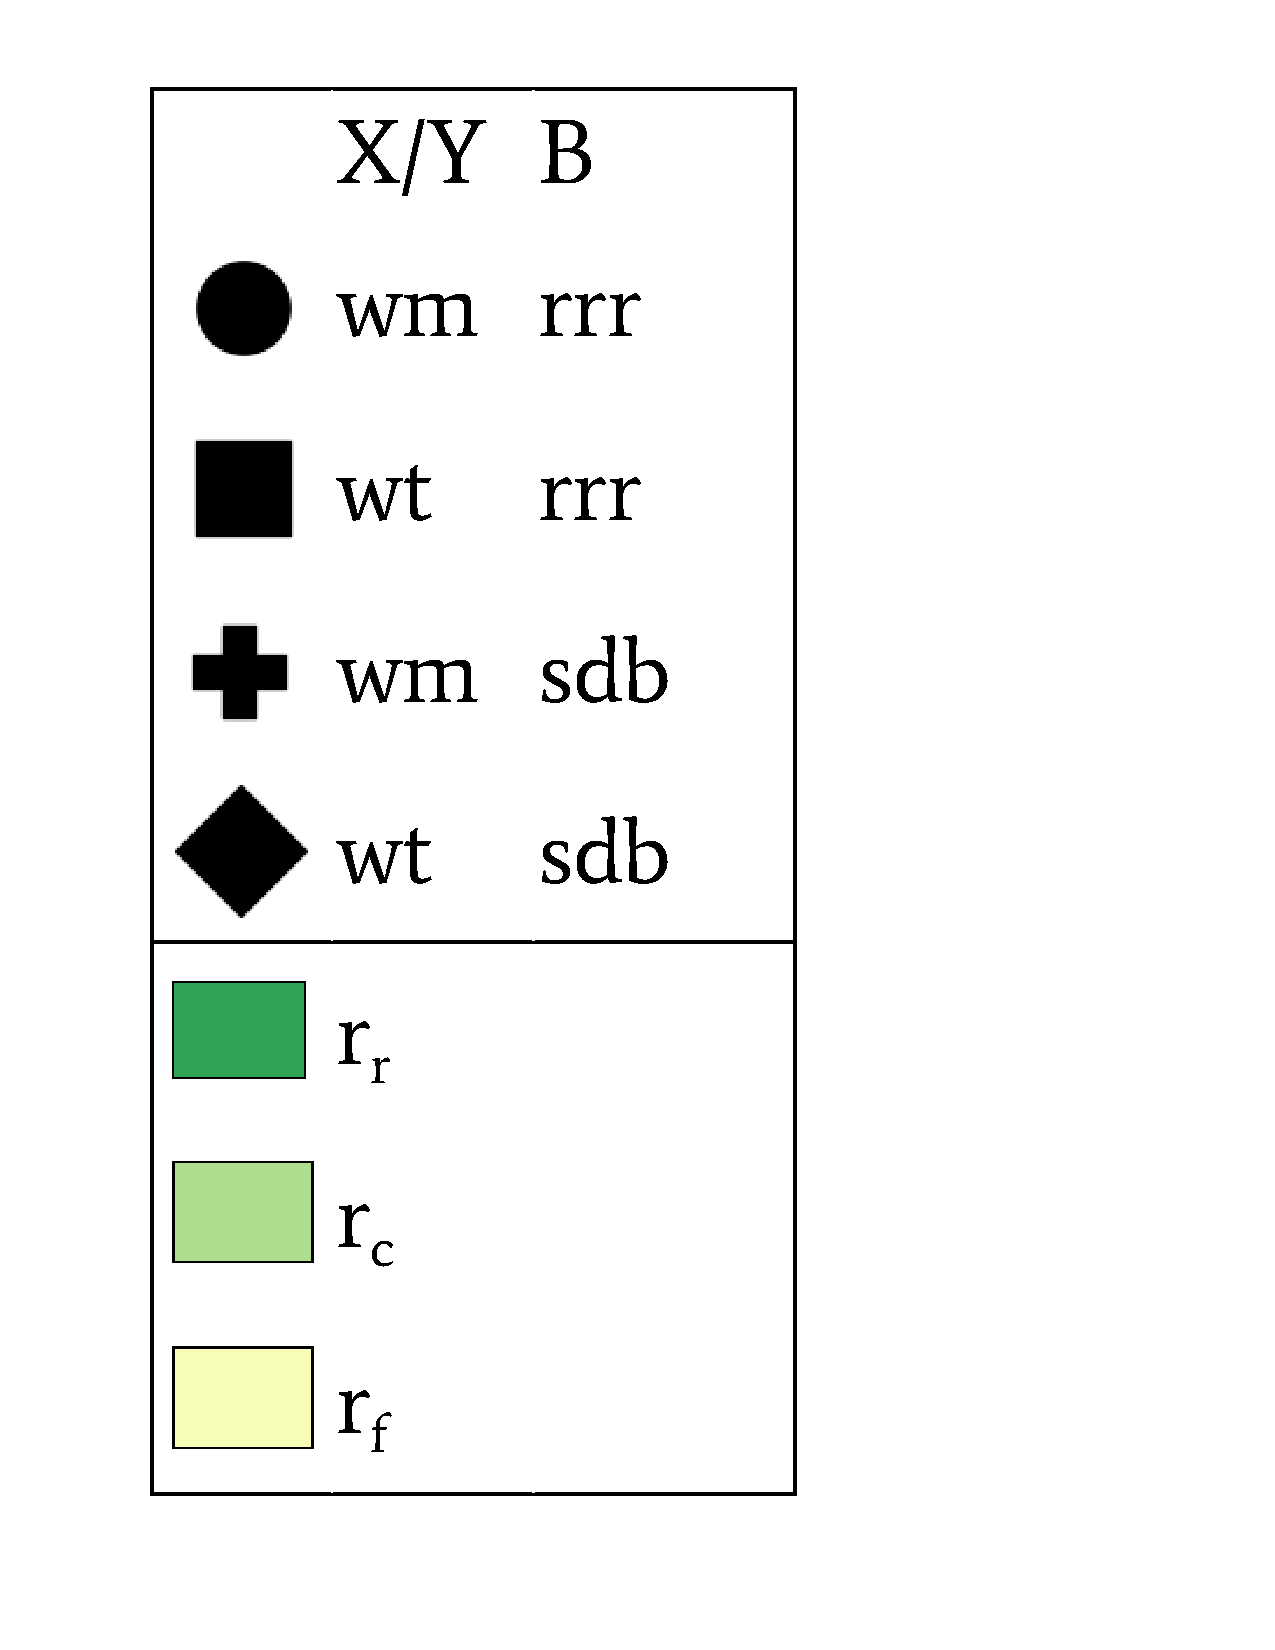
\includegraphics[scale=.15, clip, trim=70 0 0 0]{../img/sdsl/label.pdf}
    		\end{minipage}	
    	\end{minipage}

	\caption{BPE y Tiempo de acceso aleatorio medio para posibles estructuras compactas, por cada función de ranking, para snap-dblp.}
\end{figure}

\end{frame}

\begin{frame}
\frametitle{Resultados - Estructura compacta}

\begin{figure}
	\centering
	
    	\begin{minipage}{1\textwidth}
    		\centering
    		\begin{minipage}{0.8\textwidth}
    			\centering
    			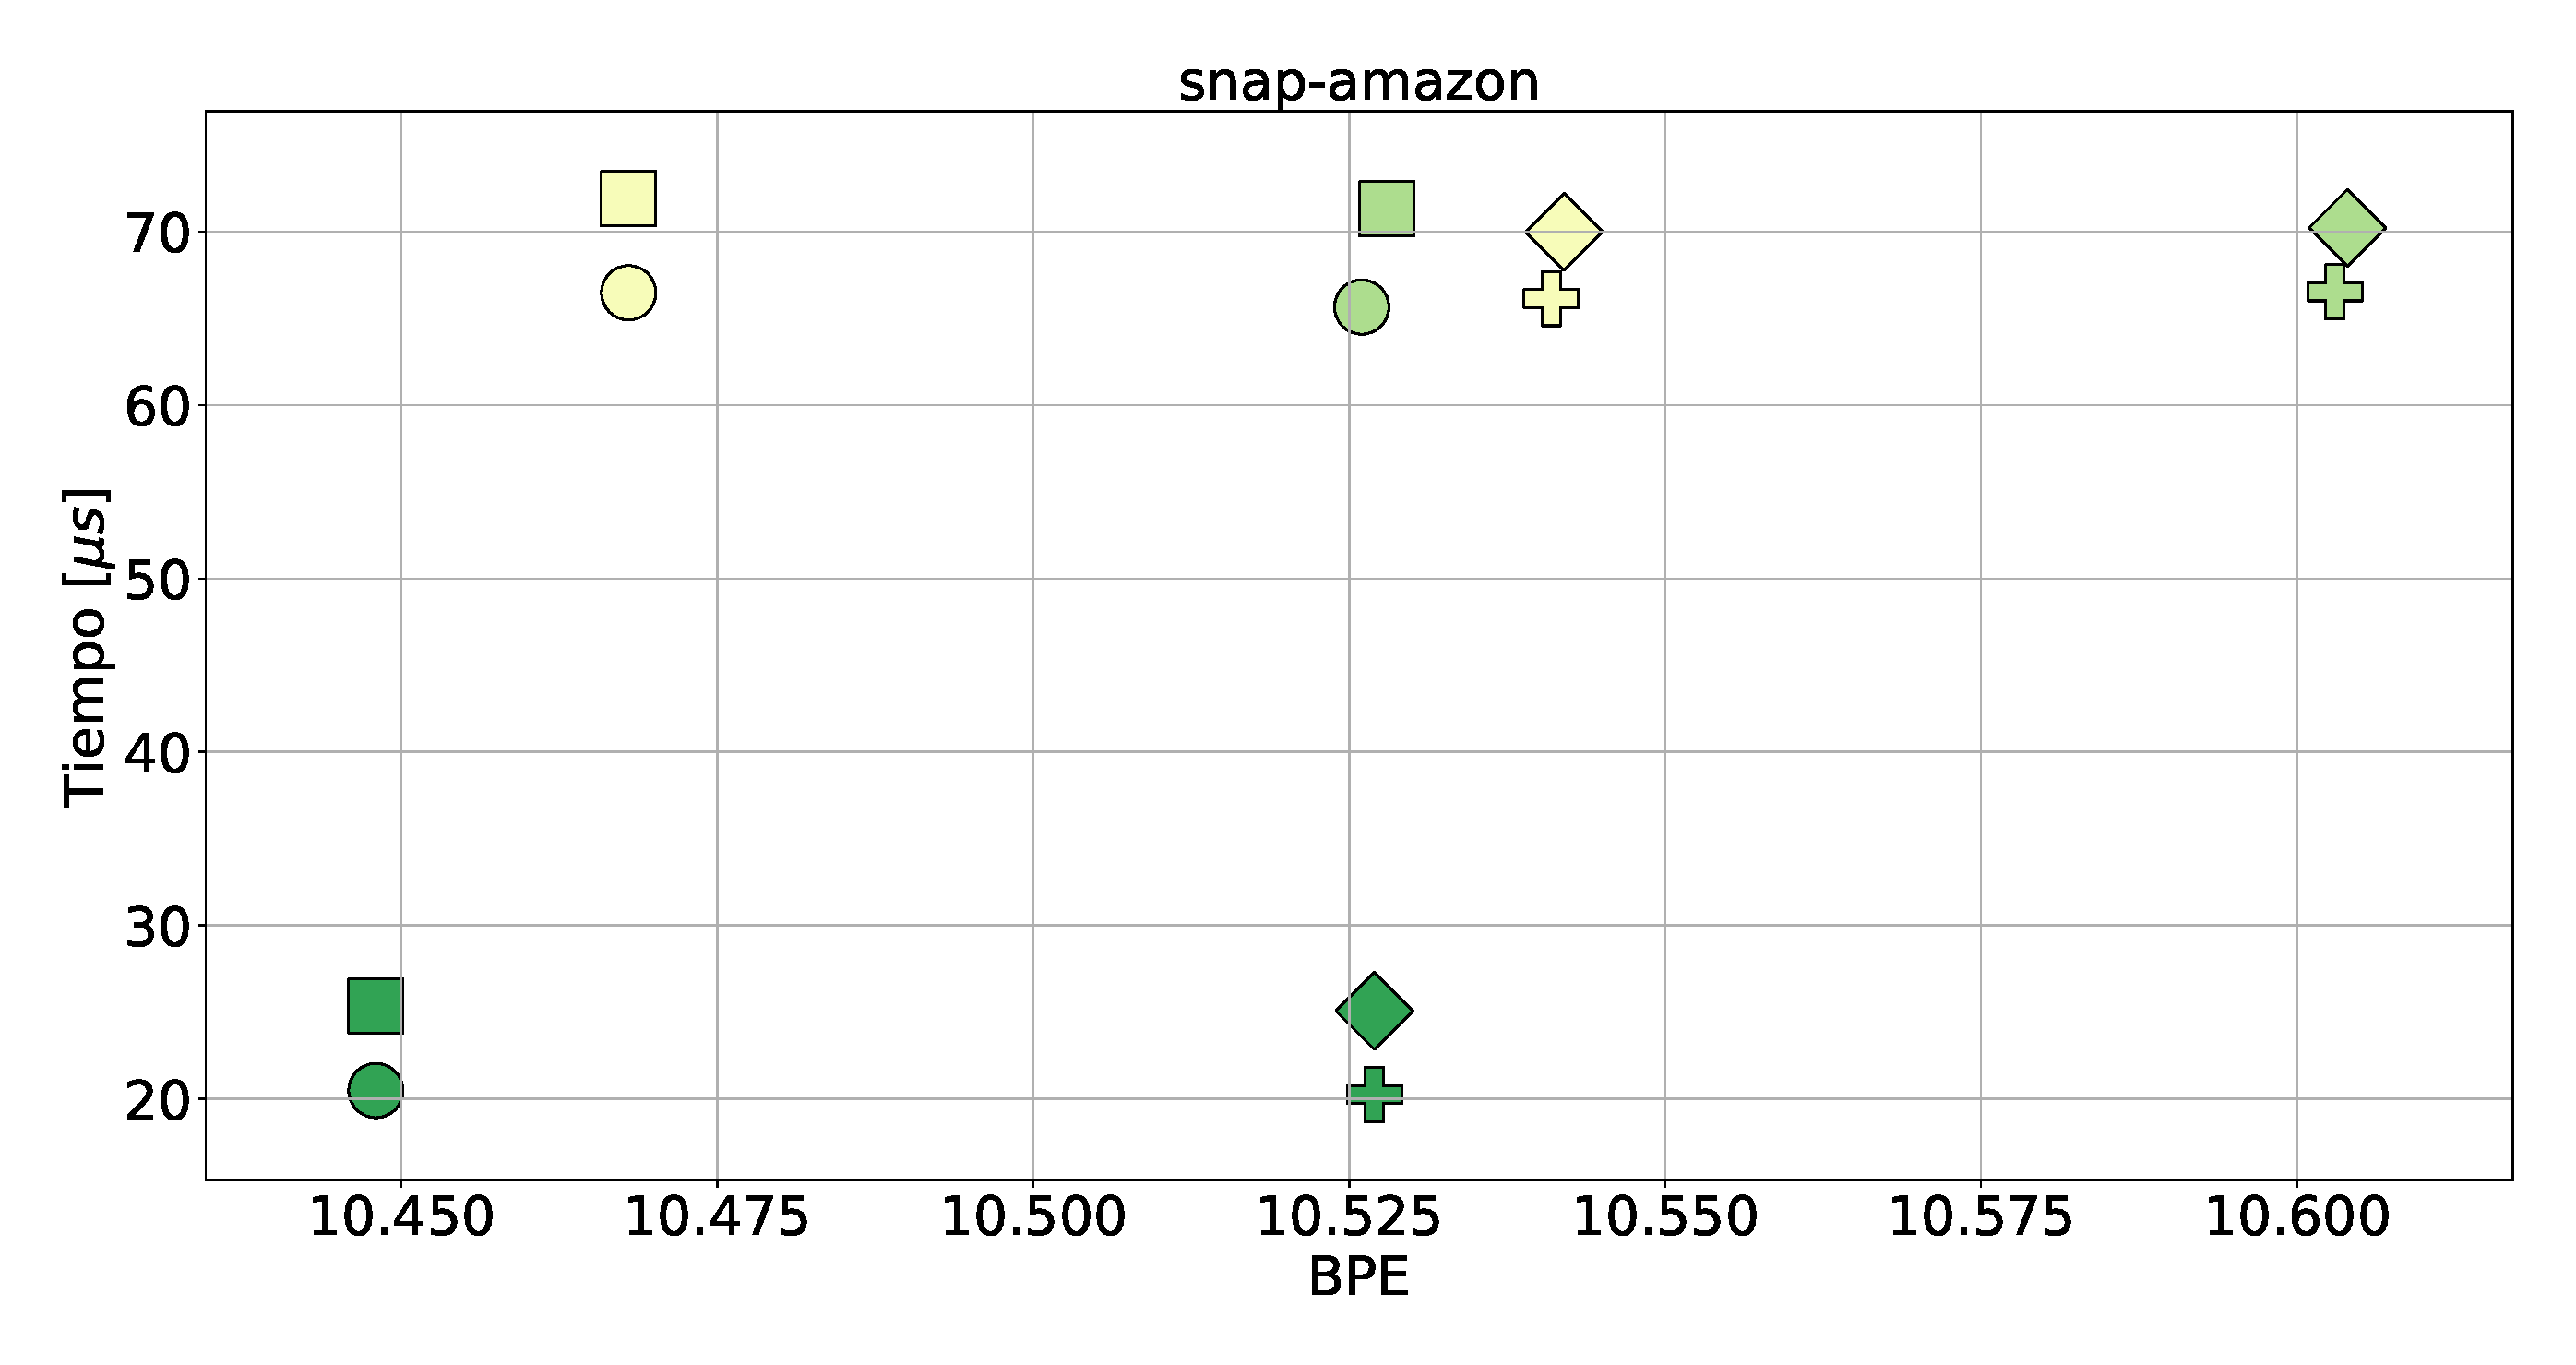
\includegraphics[width=1\linewidth]{../img/sdsl/aleatorioBig/snap-amazon.pdf}
    		\end{minipage}
    		\begin{minipage}{0.15\textwidth}
    			\centering
    			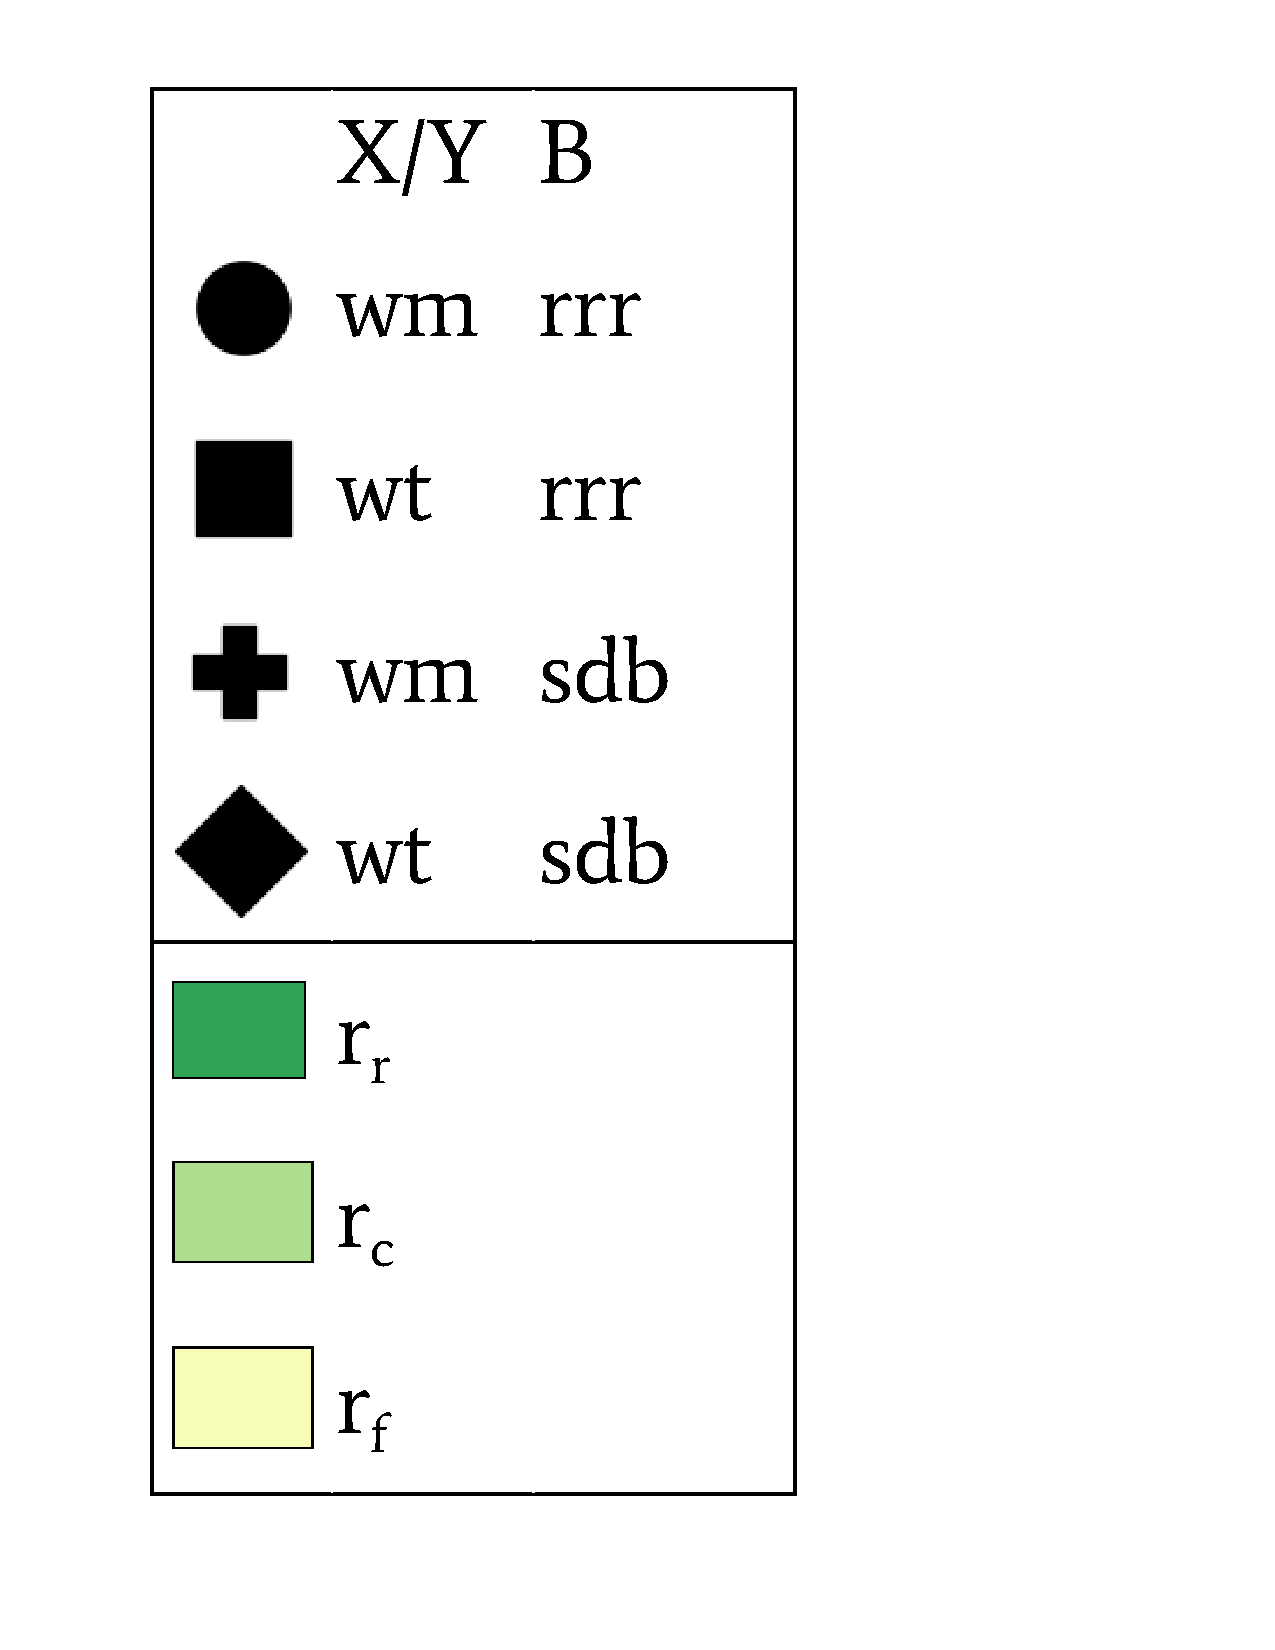
\includegraphics[scale=.15, clip, trim=70 0 0 0]{../img/sdsl/label.pdf}
    		\end{minipage}	
    	\end{minipage}

	\caption{BPE y Tiempo de acceso aleatorio medio para posibles estructuras compactas, por cada función de ranking, para snap-amazon.}
\end{figure}

\end{frame}

\begin{frame}
\frametitle{Resultados - Estructura compacta}

\begin{figure}
	\centering
	
    	\begin{minipage}{1\textwidth}
    		\centering
    		\begin{minipage}{0.8\textwidth}
    			\centering
    			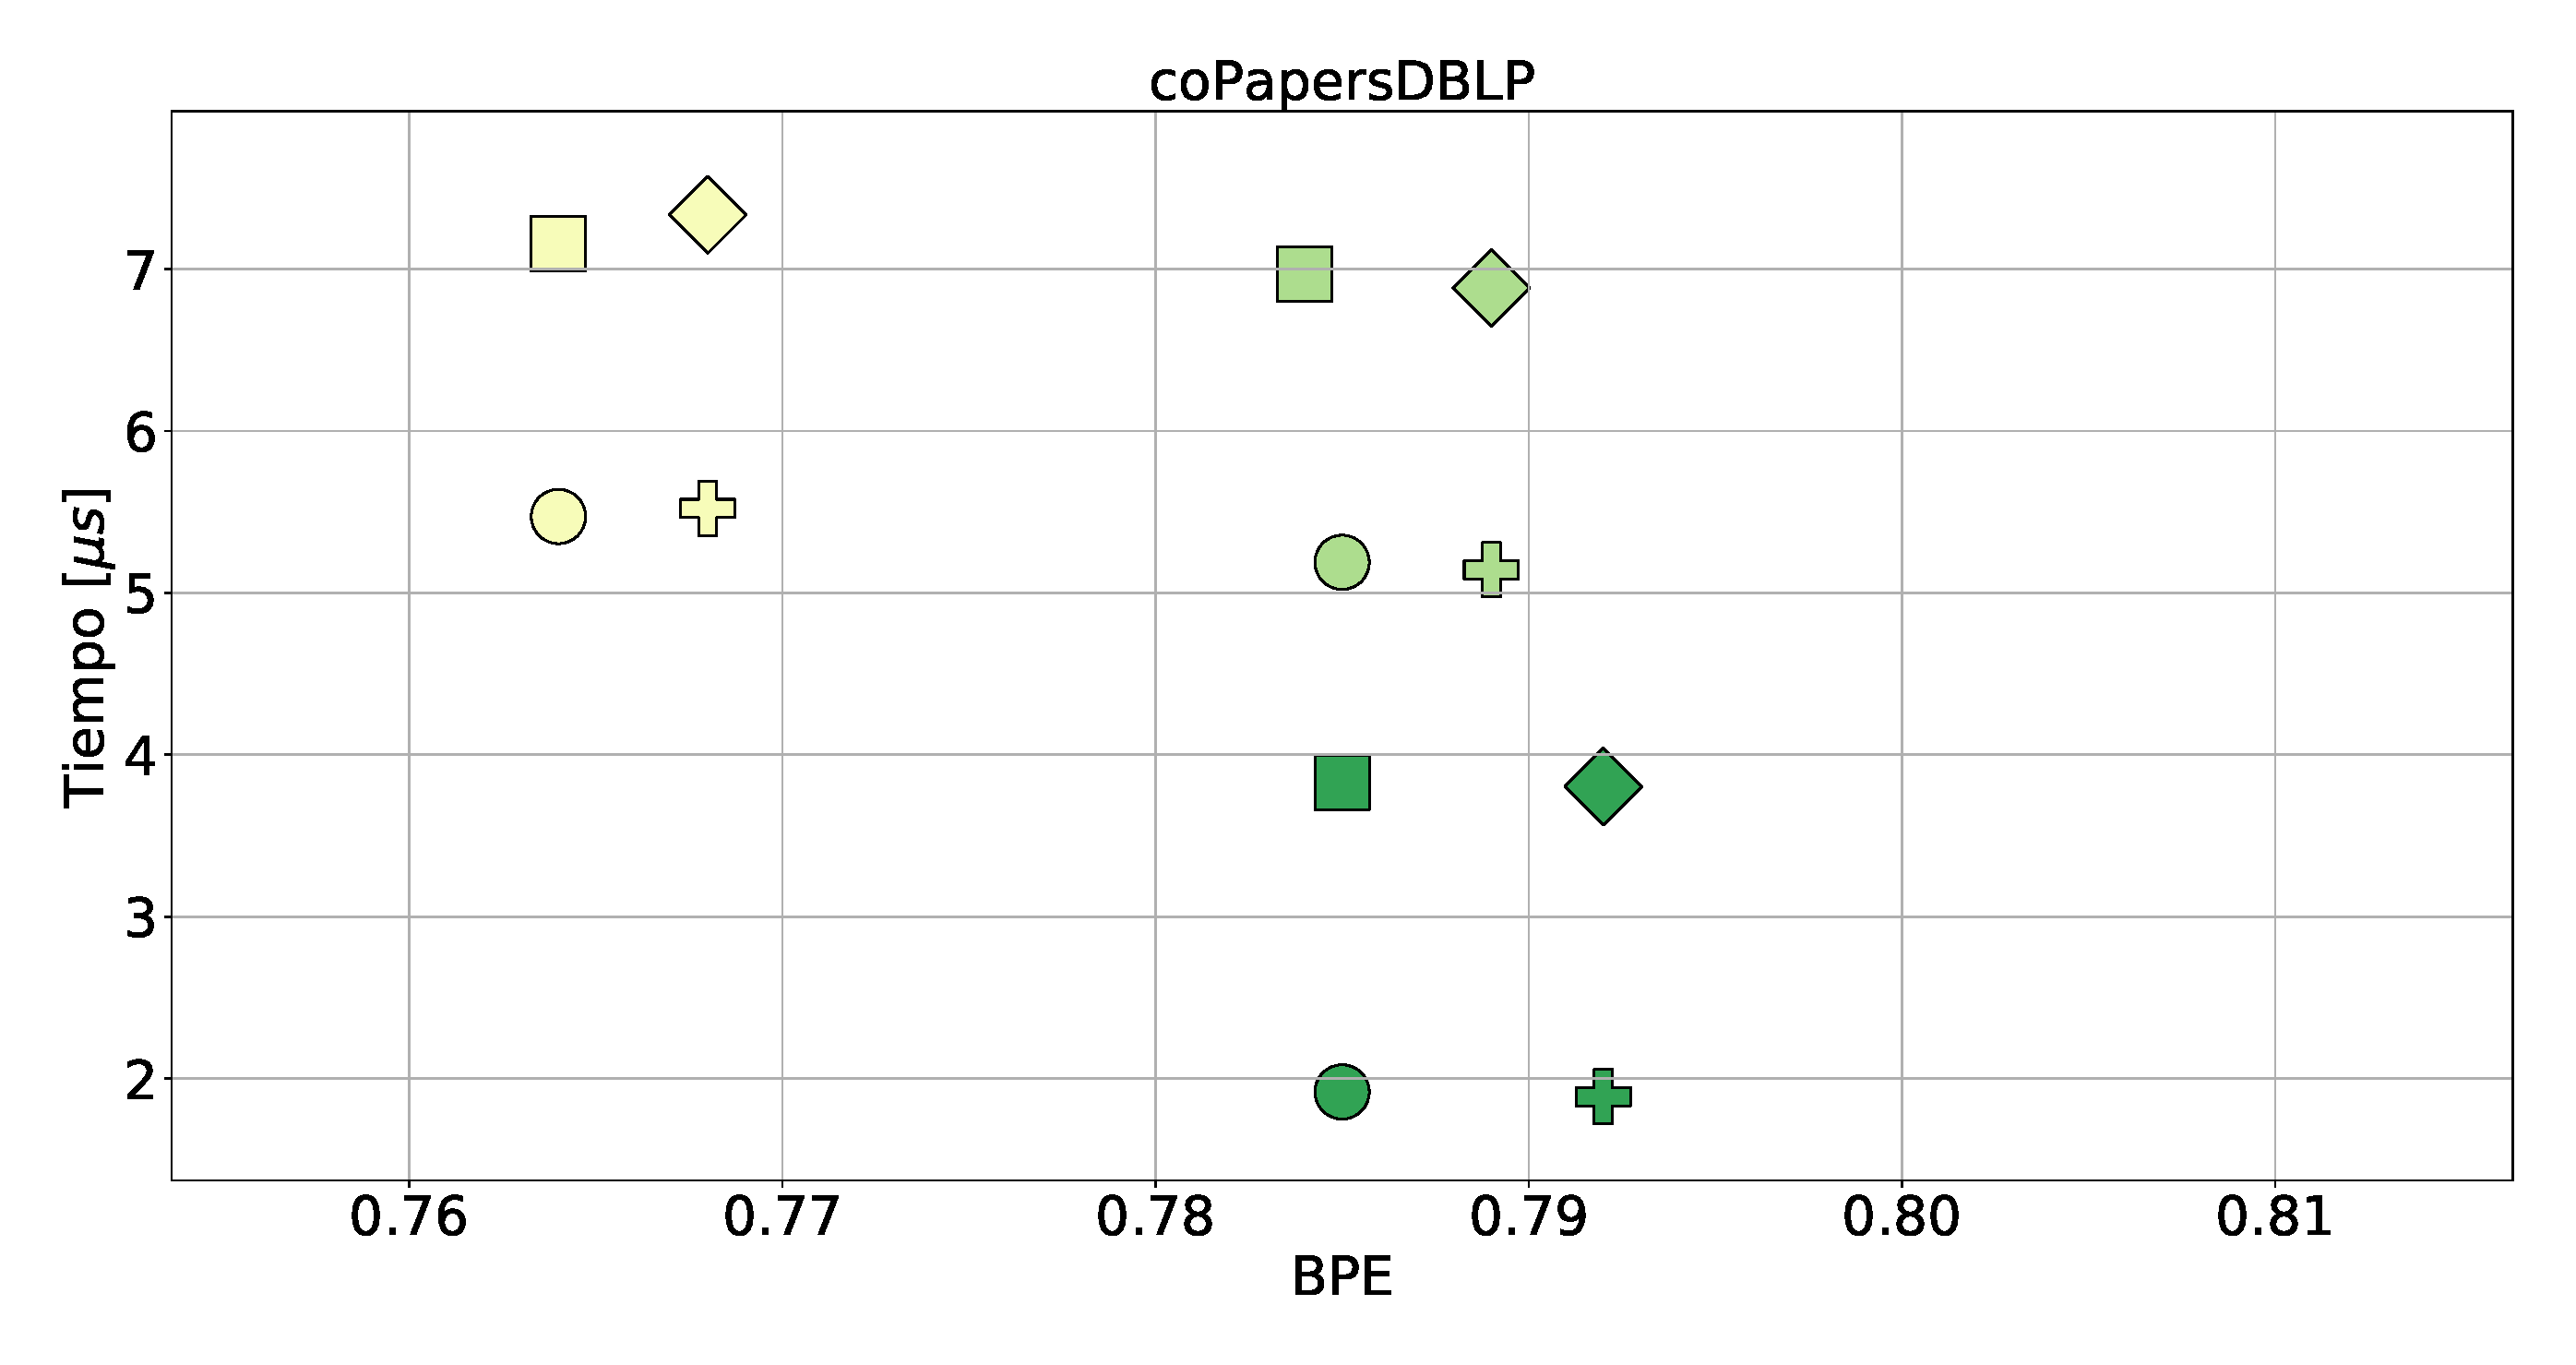
\includegraphics[width=1\linewidth]{../img/sdsl/aleatorioBig/coPapersDBLP.pdf}
    		\end{minipage}
    		\begin{minipage}{0.15\textwidth}
    			\centering
    			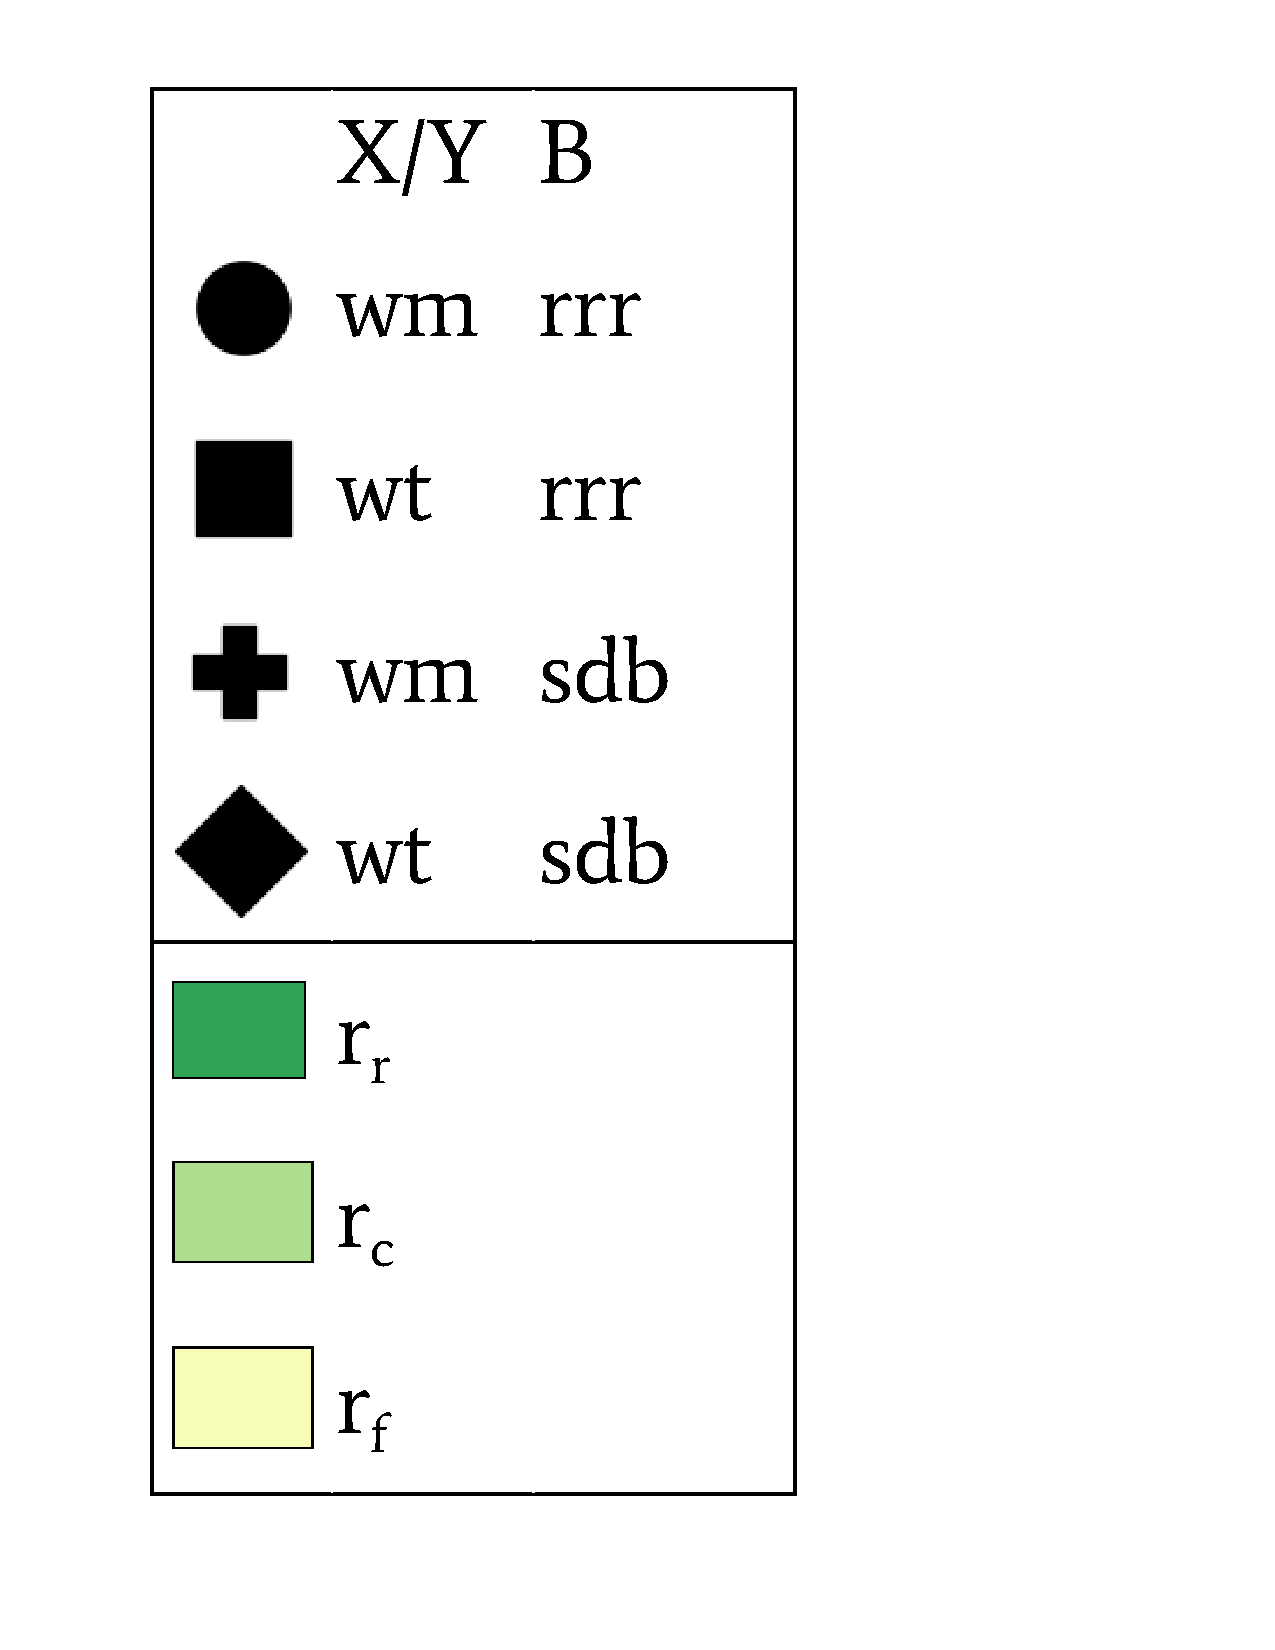
\includegraphics[scale=.15, clip, trim=70 0 0 0]{../img/sdsl/label.pdf}
    		\end{minipage}	
    	\end{minipage}

	\caption{BPE y Tiempo de acceso aleatorio medio para posibles estructuras compactas, por cada función de ranking, para coPapersDBLP.}
\end{figure}

\end{frame}

\begin{frame}
\frametitle{Resultados - Estructura compacta}

\begin{figure}
	\centering
	
    	\begin{minipage}{1\textwidth}
    		\centering
    		\begin{minipage}{0.8\textwidth}
    			\centering
    			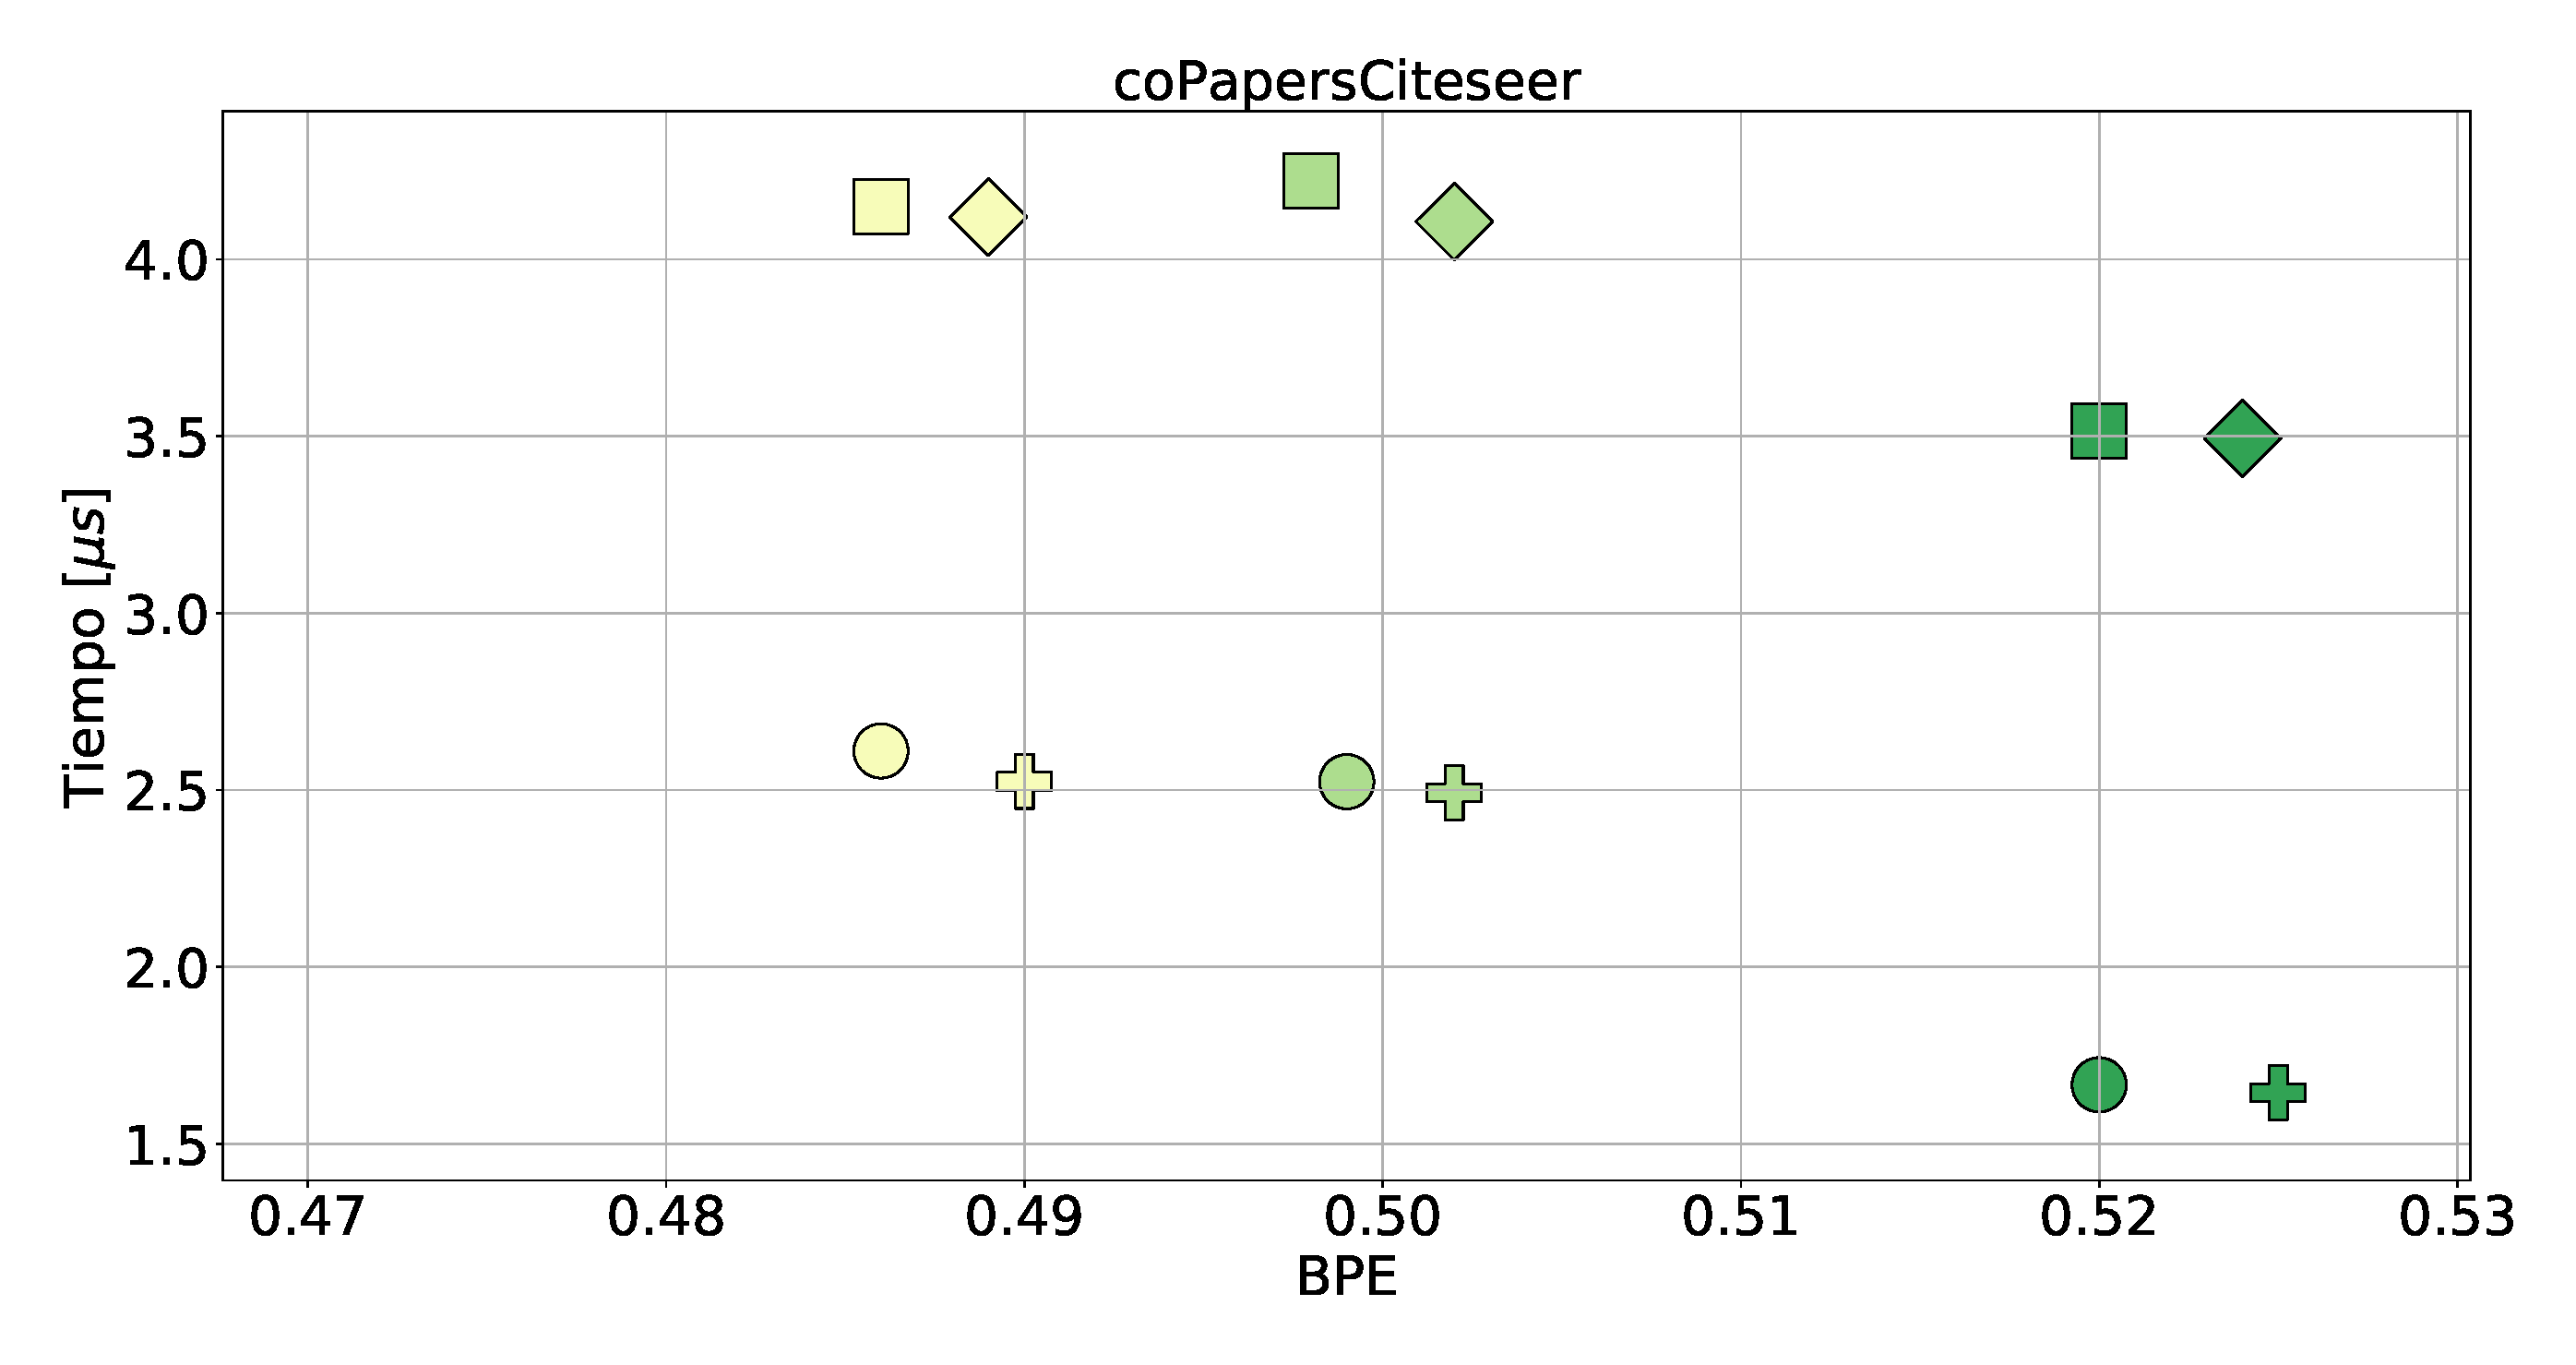
\includegraphics[width=1\linewidth]{../img/sdsl/aleatorioBig/coPapersCiteseer.pdf}
    		\end{minipage}
    		\begin{minipage}{0.15\textwidth}
    			\centering
    			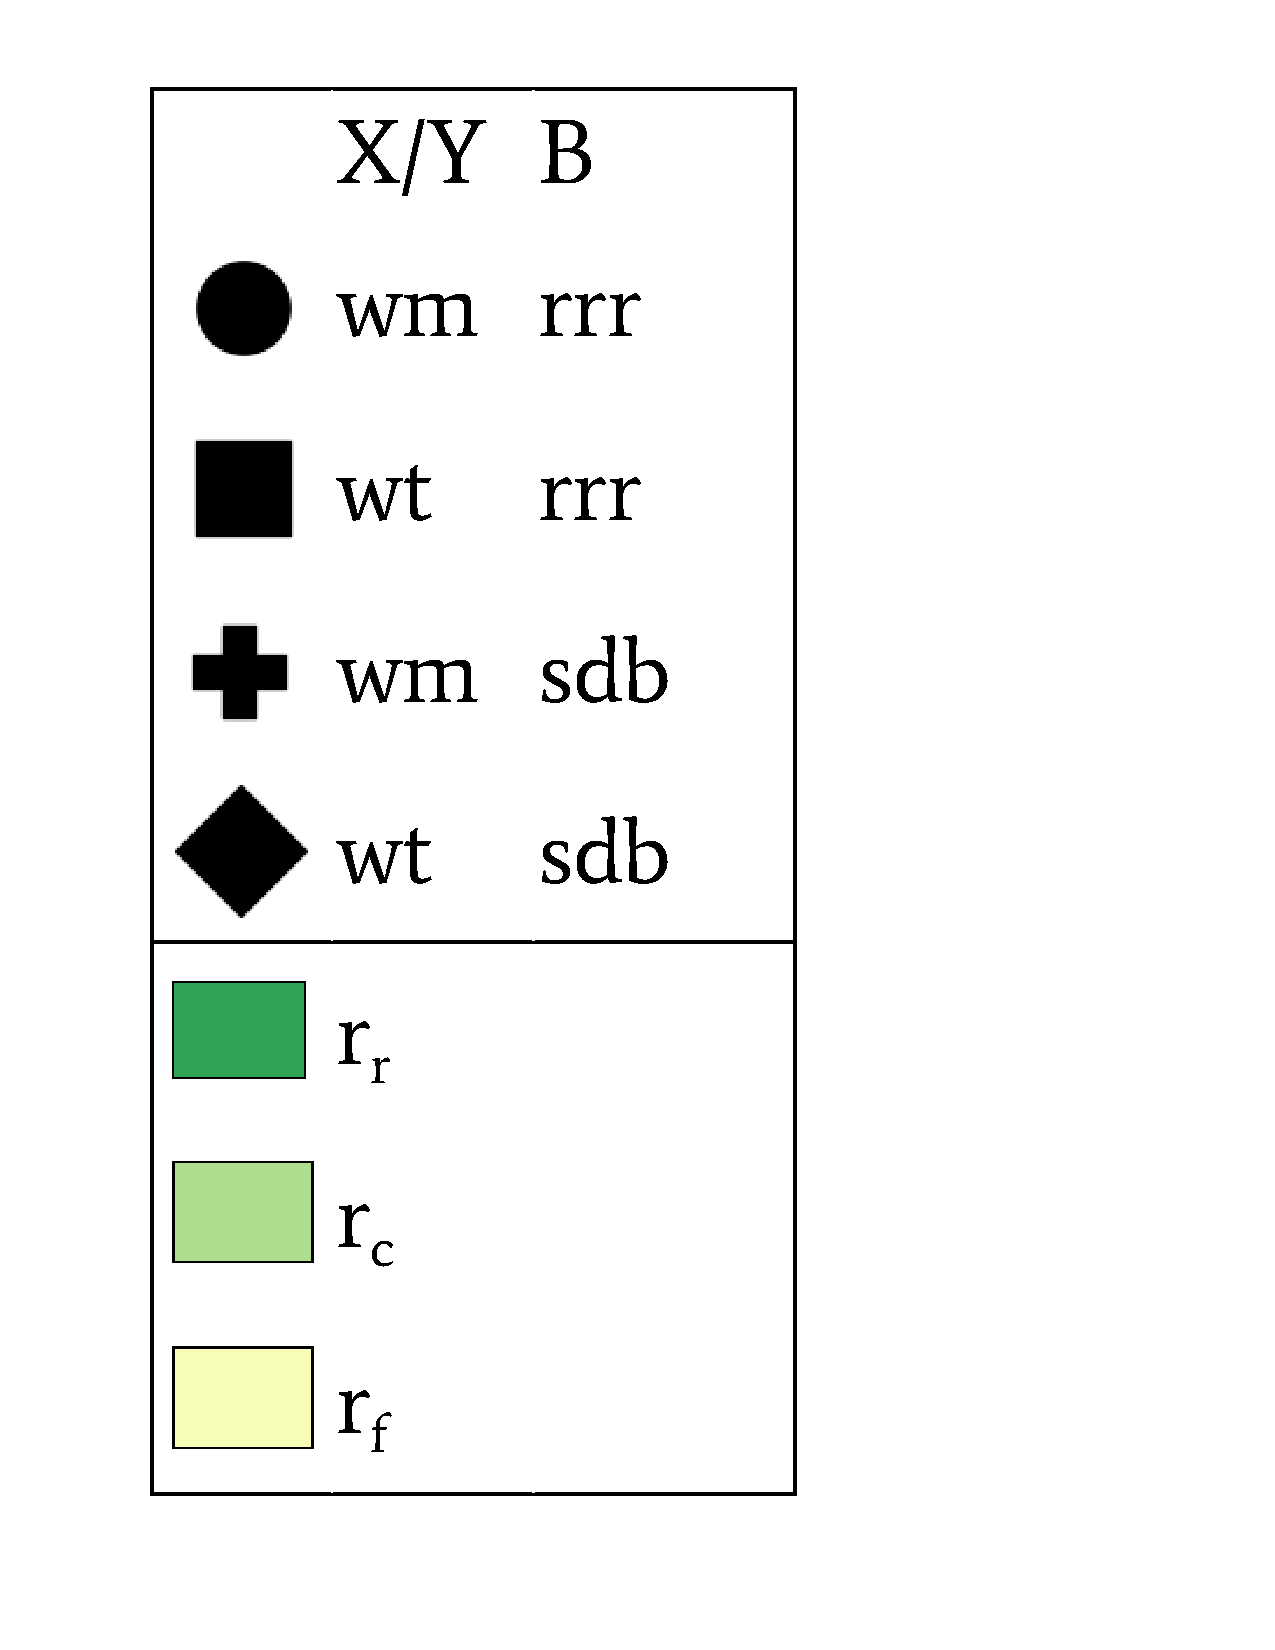
\includegraphics[scale=.15, clip, trim=70 0 0 0]{../img/sdsl/label.pdf}
    		\end{minipage}	
    	\end{minipage}

	\caption{BPE y Tiempo de acceso aleatorio medio para posibles estructuras compactas, por cada función de ranking, para coPapersCiteseer.}
\end{figure}

\end{frame}


\begin{frame}
\frametitle{Resultados - Estructura compacta}

\begin{figure}
	\centering
	
    	\begin{minipage}{1\textwidth}
    		\centering
    		\begin{minipage}{0.8\textwidth}
    			\centering
    			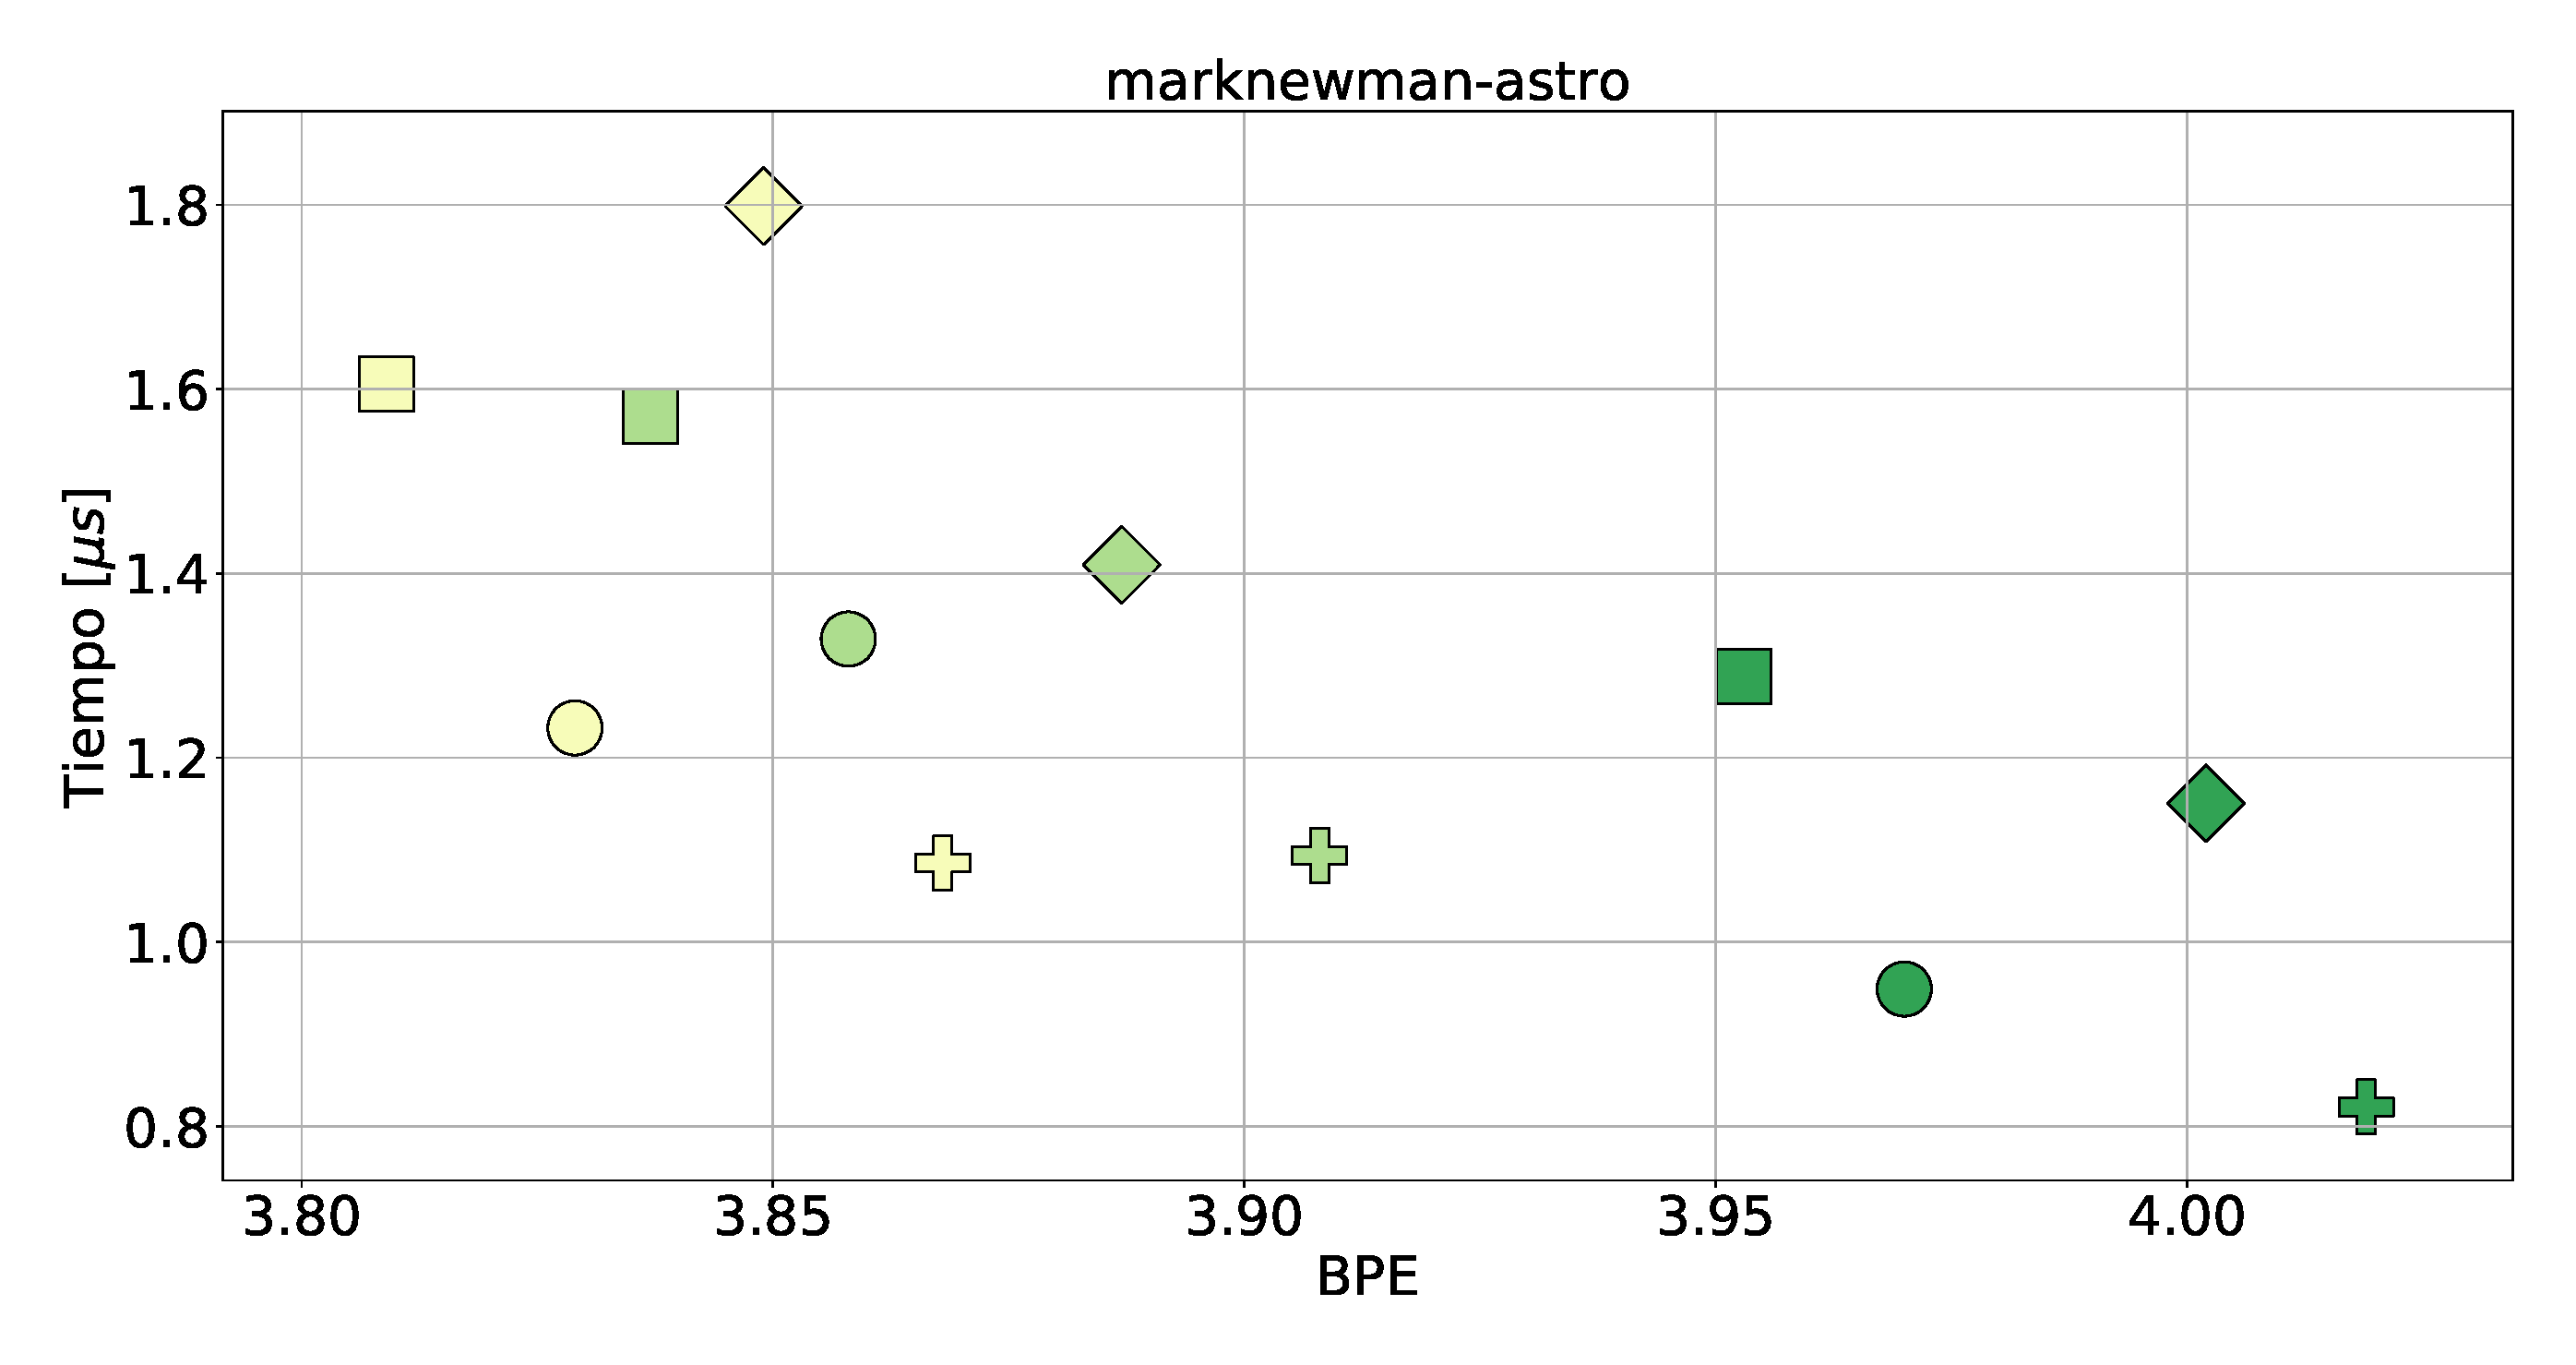
\includegraphics[width=1\linewidth]{../img/sdsl/secuencialBig/marknewman-astro.pdf}
    		\end{minipage}
    		\begin{minipage}{0.15\textwidth}
    			\centering
    			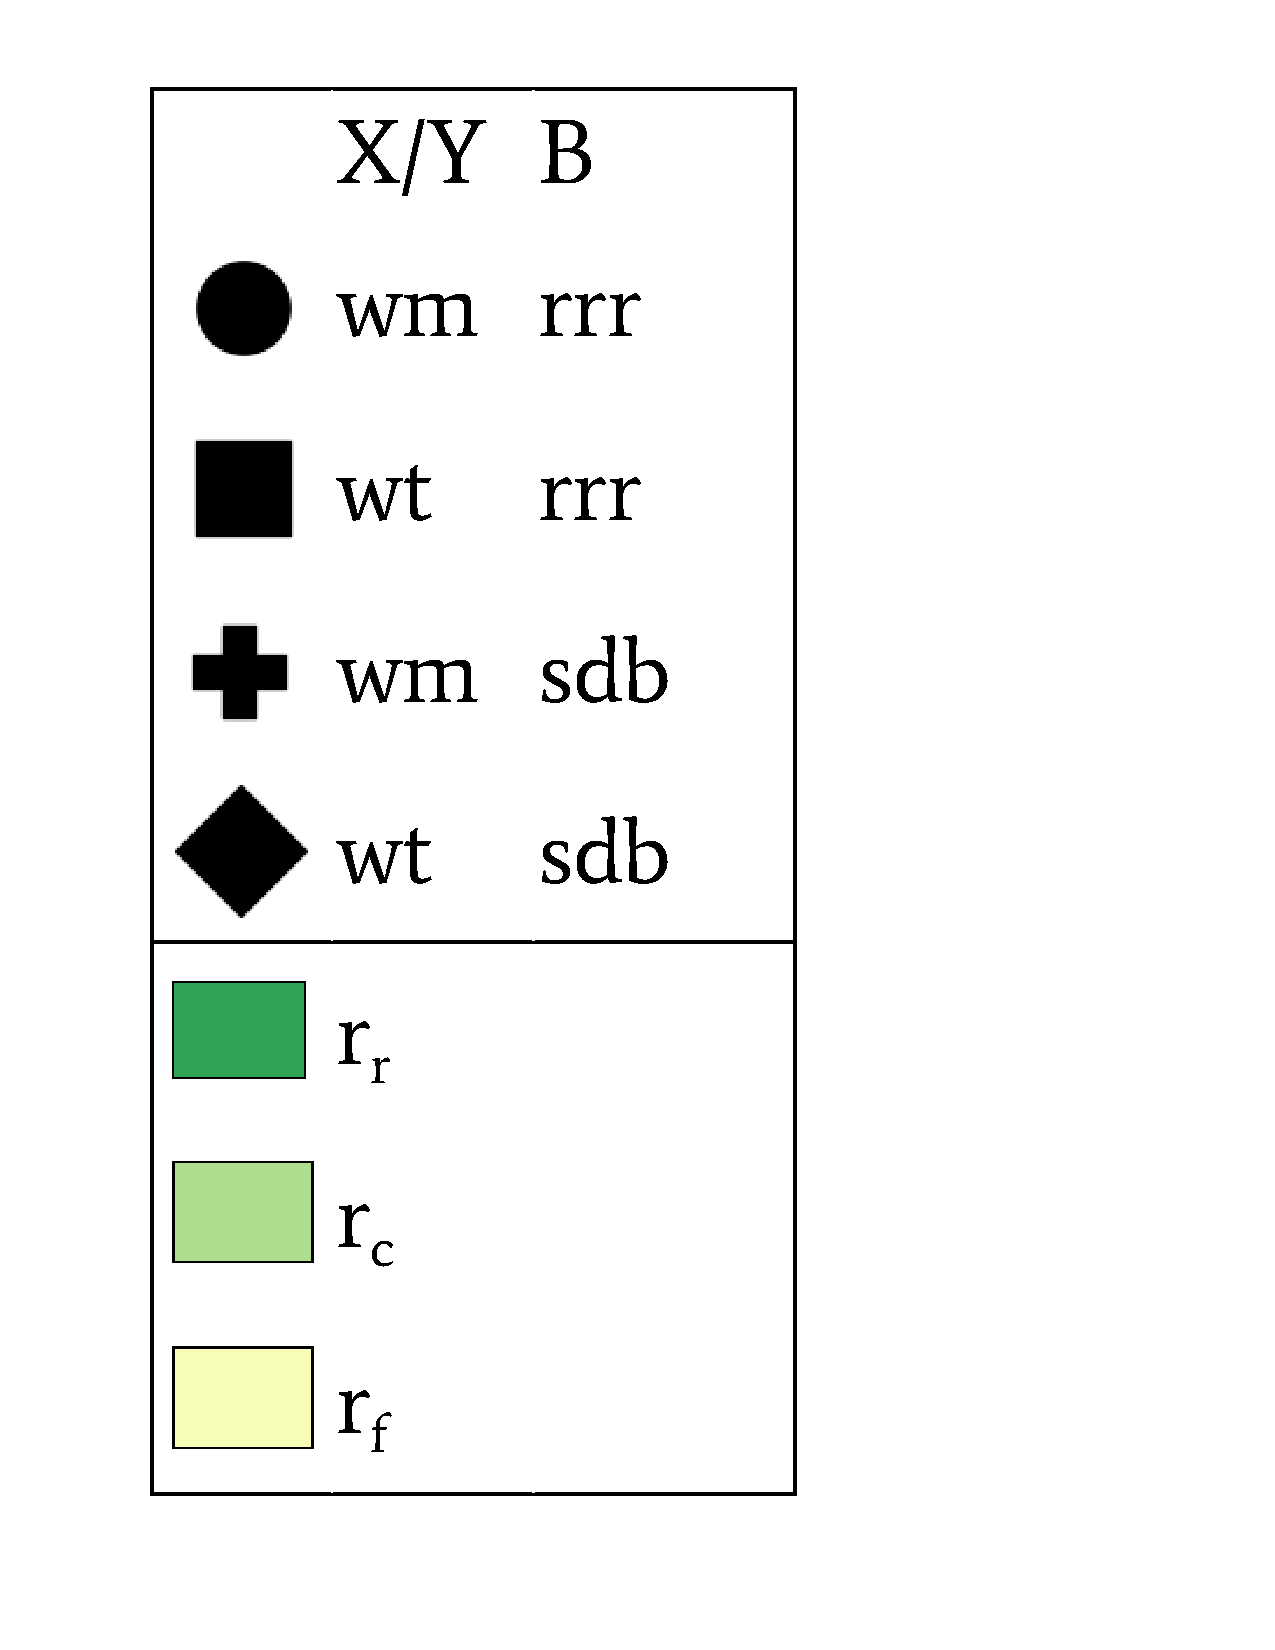
\includegraphics[scale=.15, clip, trim=70 0 0 0]{../img/sdsl/label.pdf}
    		\end{minipage}	
    	\end{minipage}

	\caption{BPE y Tiempo de acceso secuencial medio para posibles estructuras compactas, por cada función de ranking, para marknewman-astro.}
\end{figure}

\end{frame}

\begin{frame}
\frametitle{Resultados - Estructura compacta}

\begin{figure}
	\centering
	
    	\begin{minipage}{1\textwidth}
    		\centering
    		\begin{minipage}{0.8\textwidth}
    			\centering
    			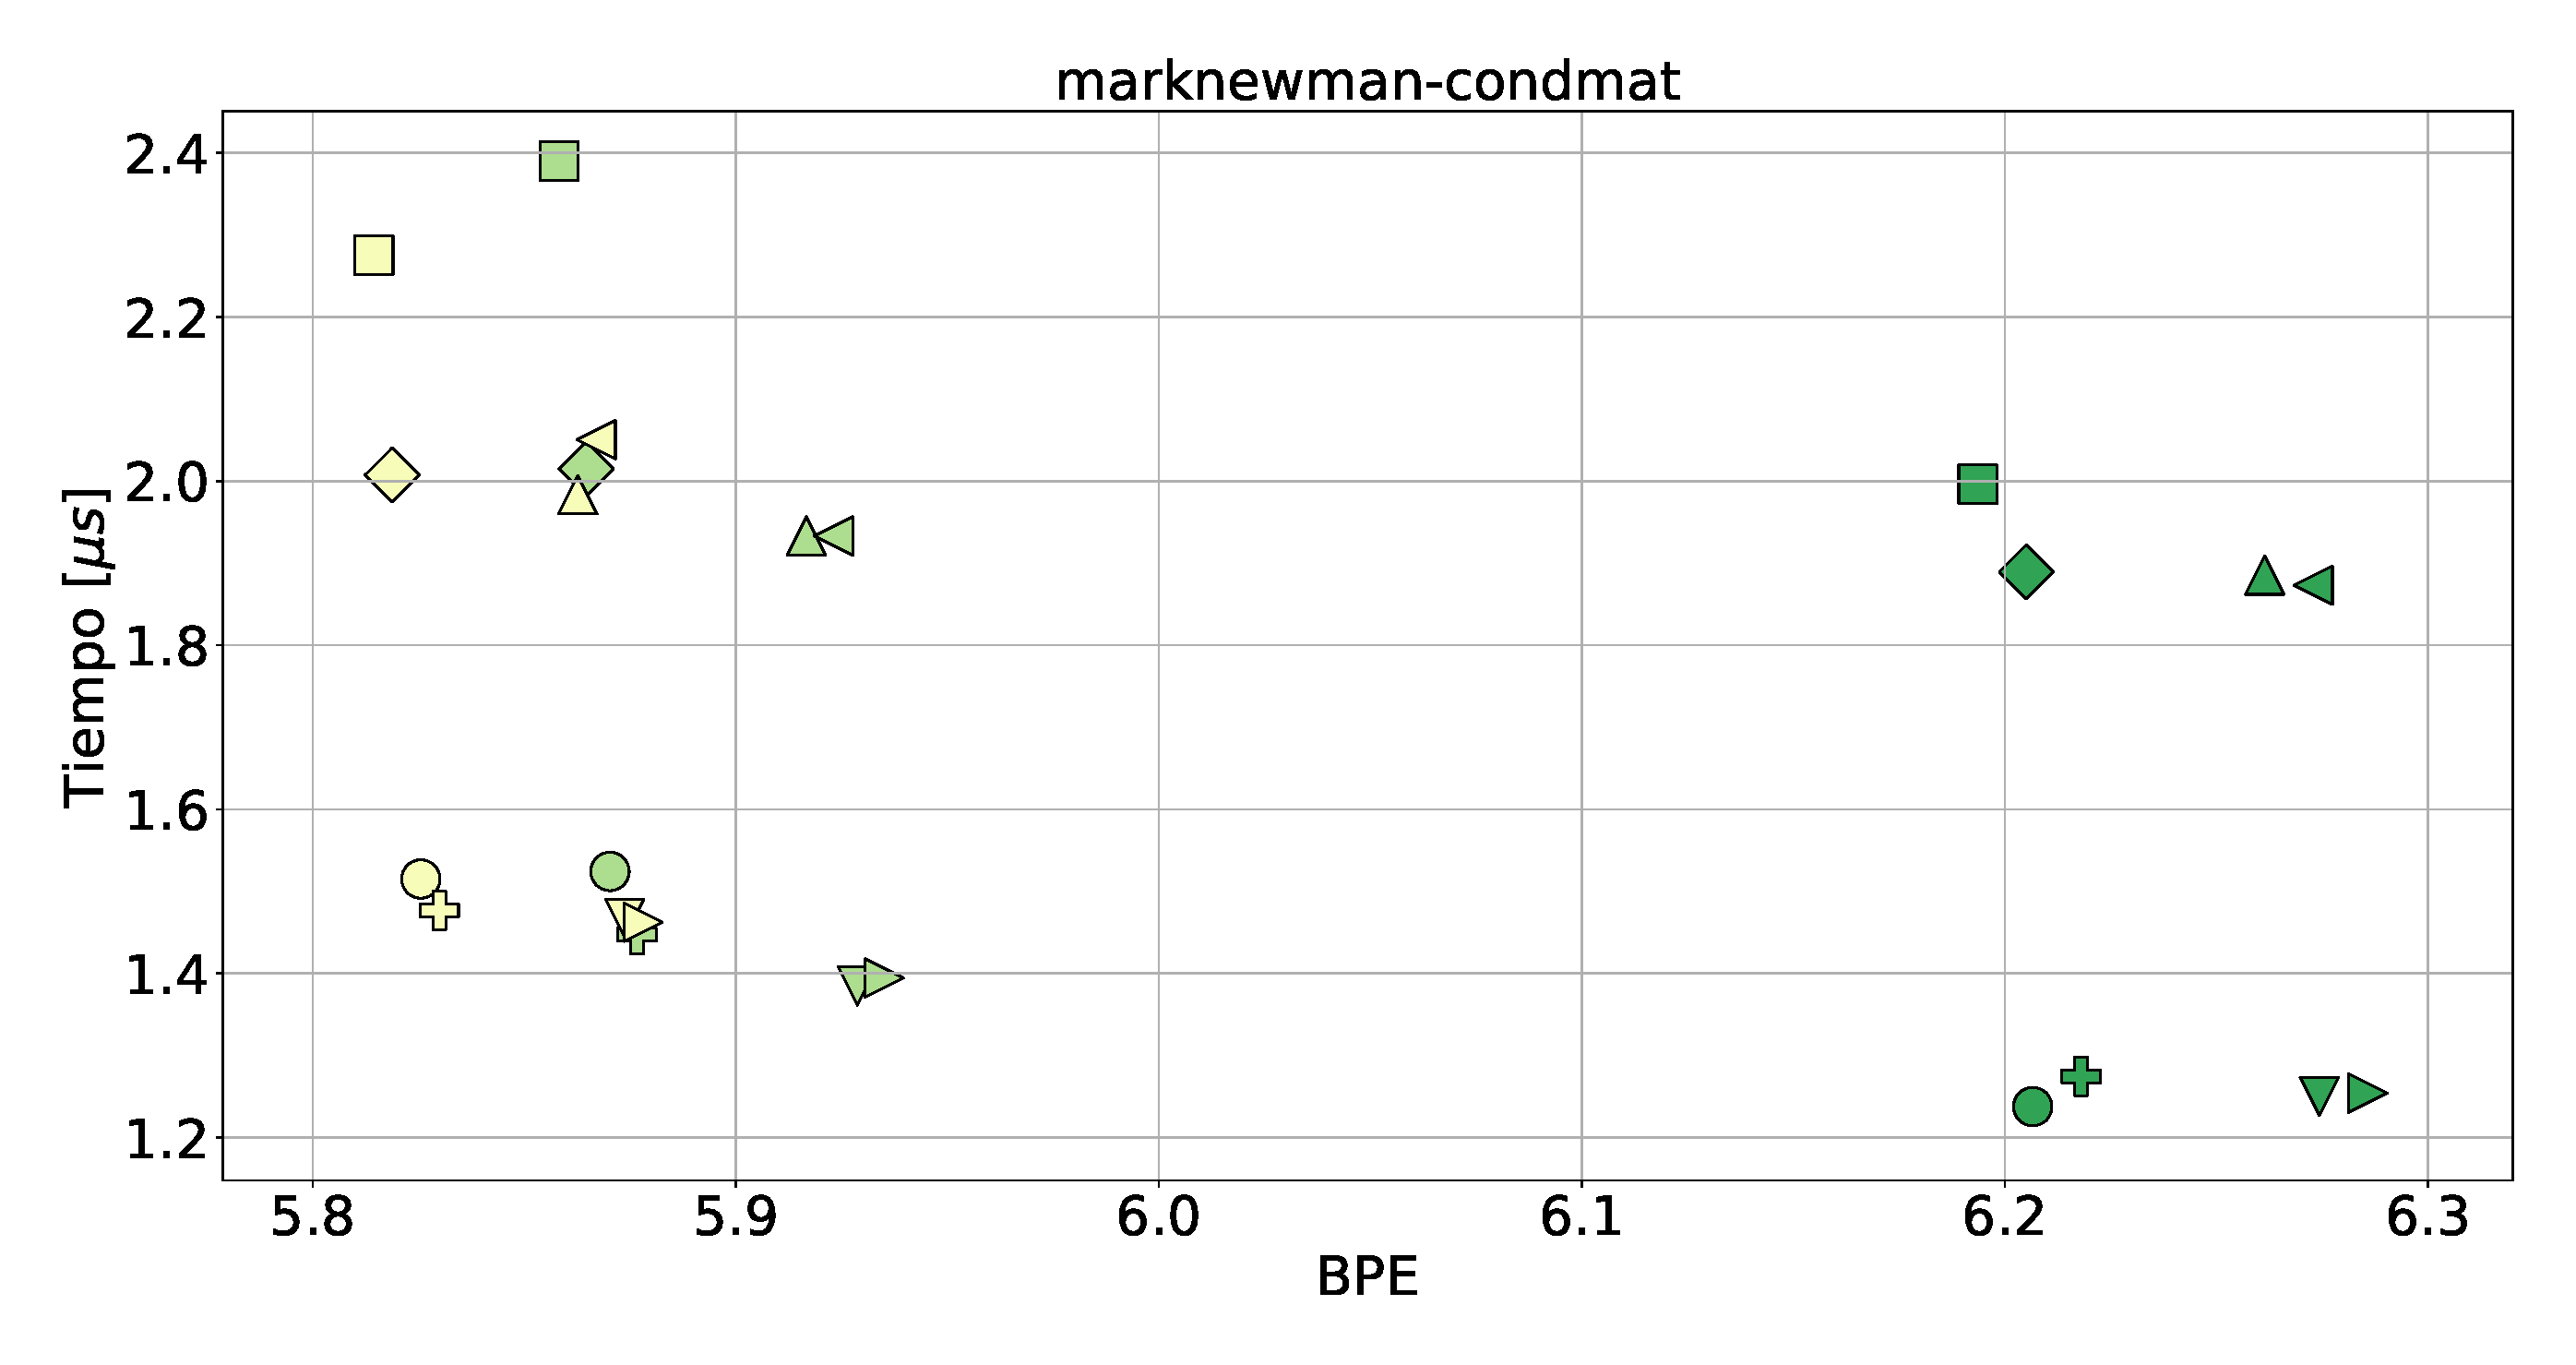
\includegraphics[width=1\linewidth]{../img/sdsl/secuencialBig/marknewman-condmat.pdf}
    		\end{minipage}
    		\begin{minipage}{0.15\textwidth}
    			\centering
    			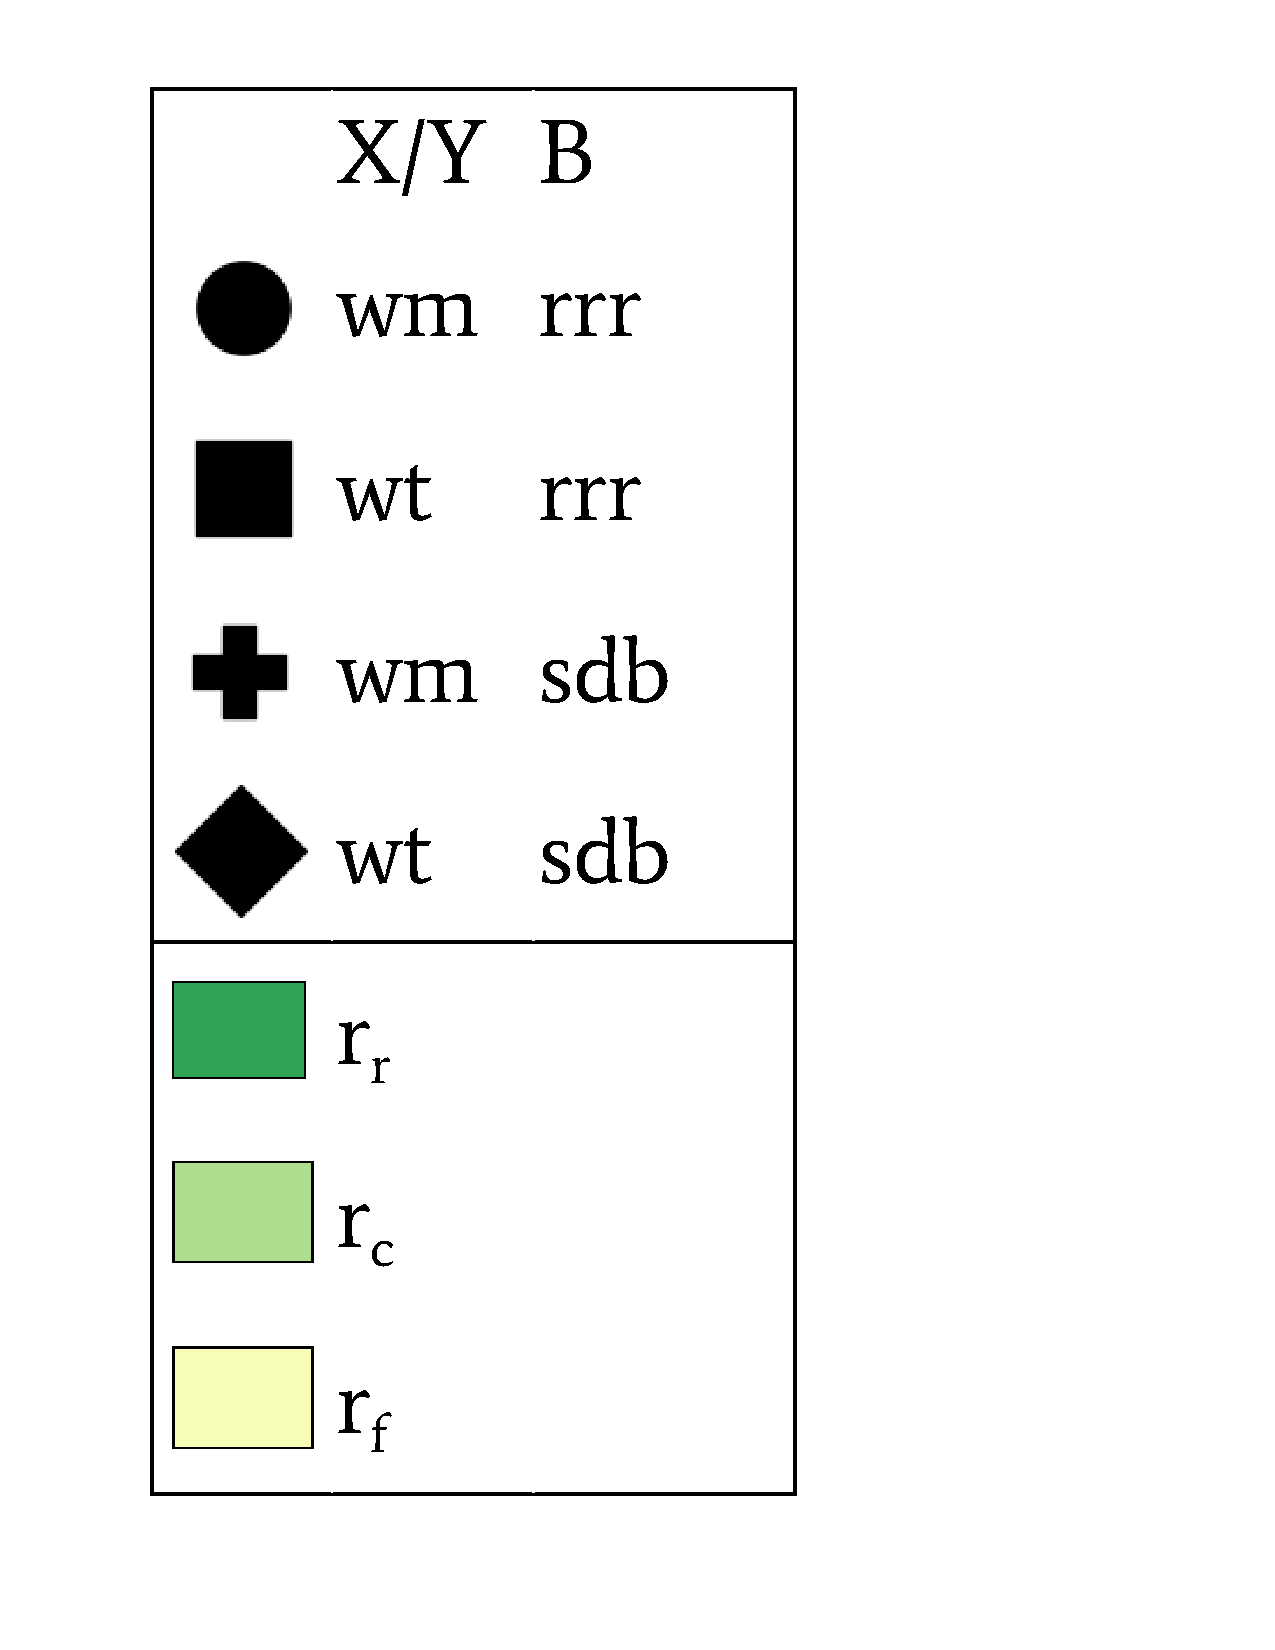
\includegraphics[scale=.15, clip, trim=70 0 0 0]{../img/sdsl/label.pdf}
    		\end{minipage}	
    	\end{minipage}

	\caption{BPE y Tiempo de acceso secuencial medio para posibles estructuras compactas, por cada función de ranking, para marknewman-condmat.}
\end{figure}

\end{frame}

\begin{frame}
\frametitle{Resultados - Estructura compacta}

\begin{figure}
	\centering
	
    	\begin{minipage}{1\textwidth}
    		\centering
    		\begin{minipage}{0.8\textwidth}
    			\centering
    			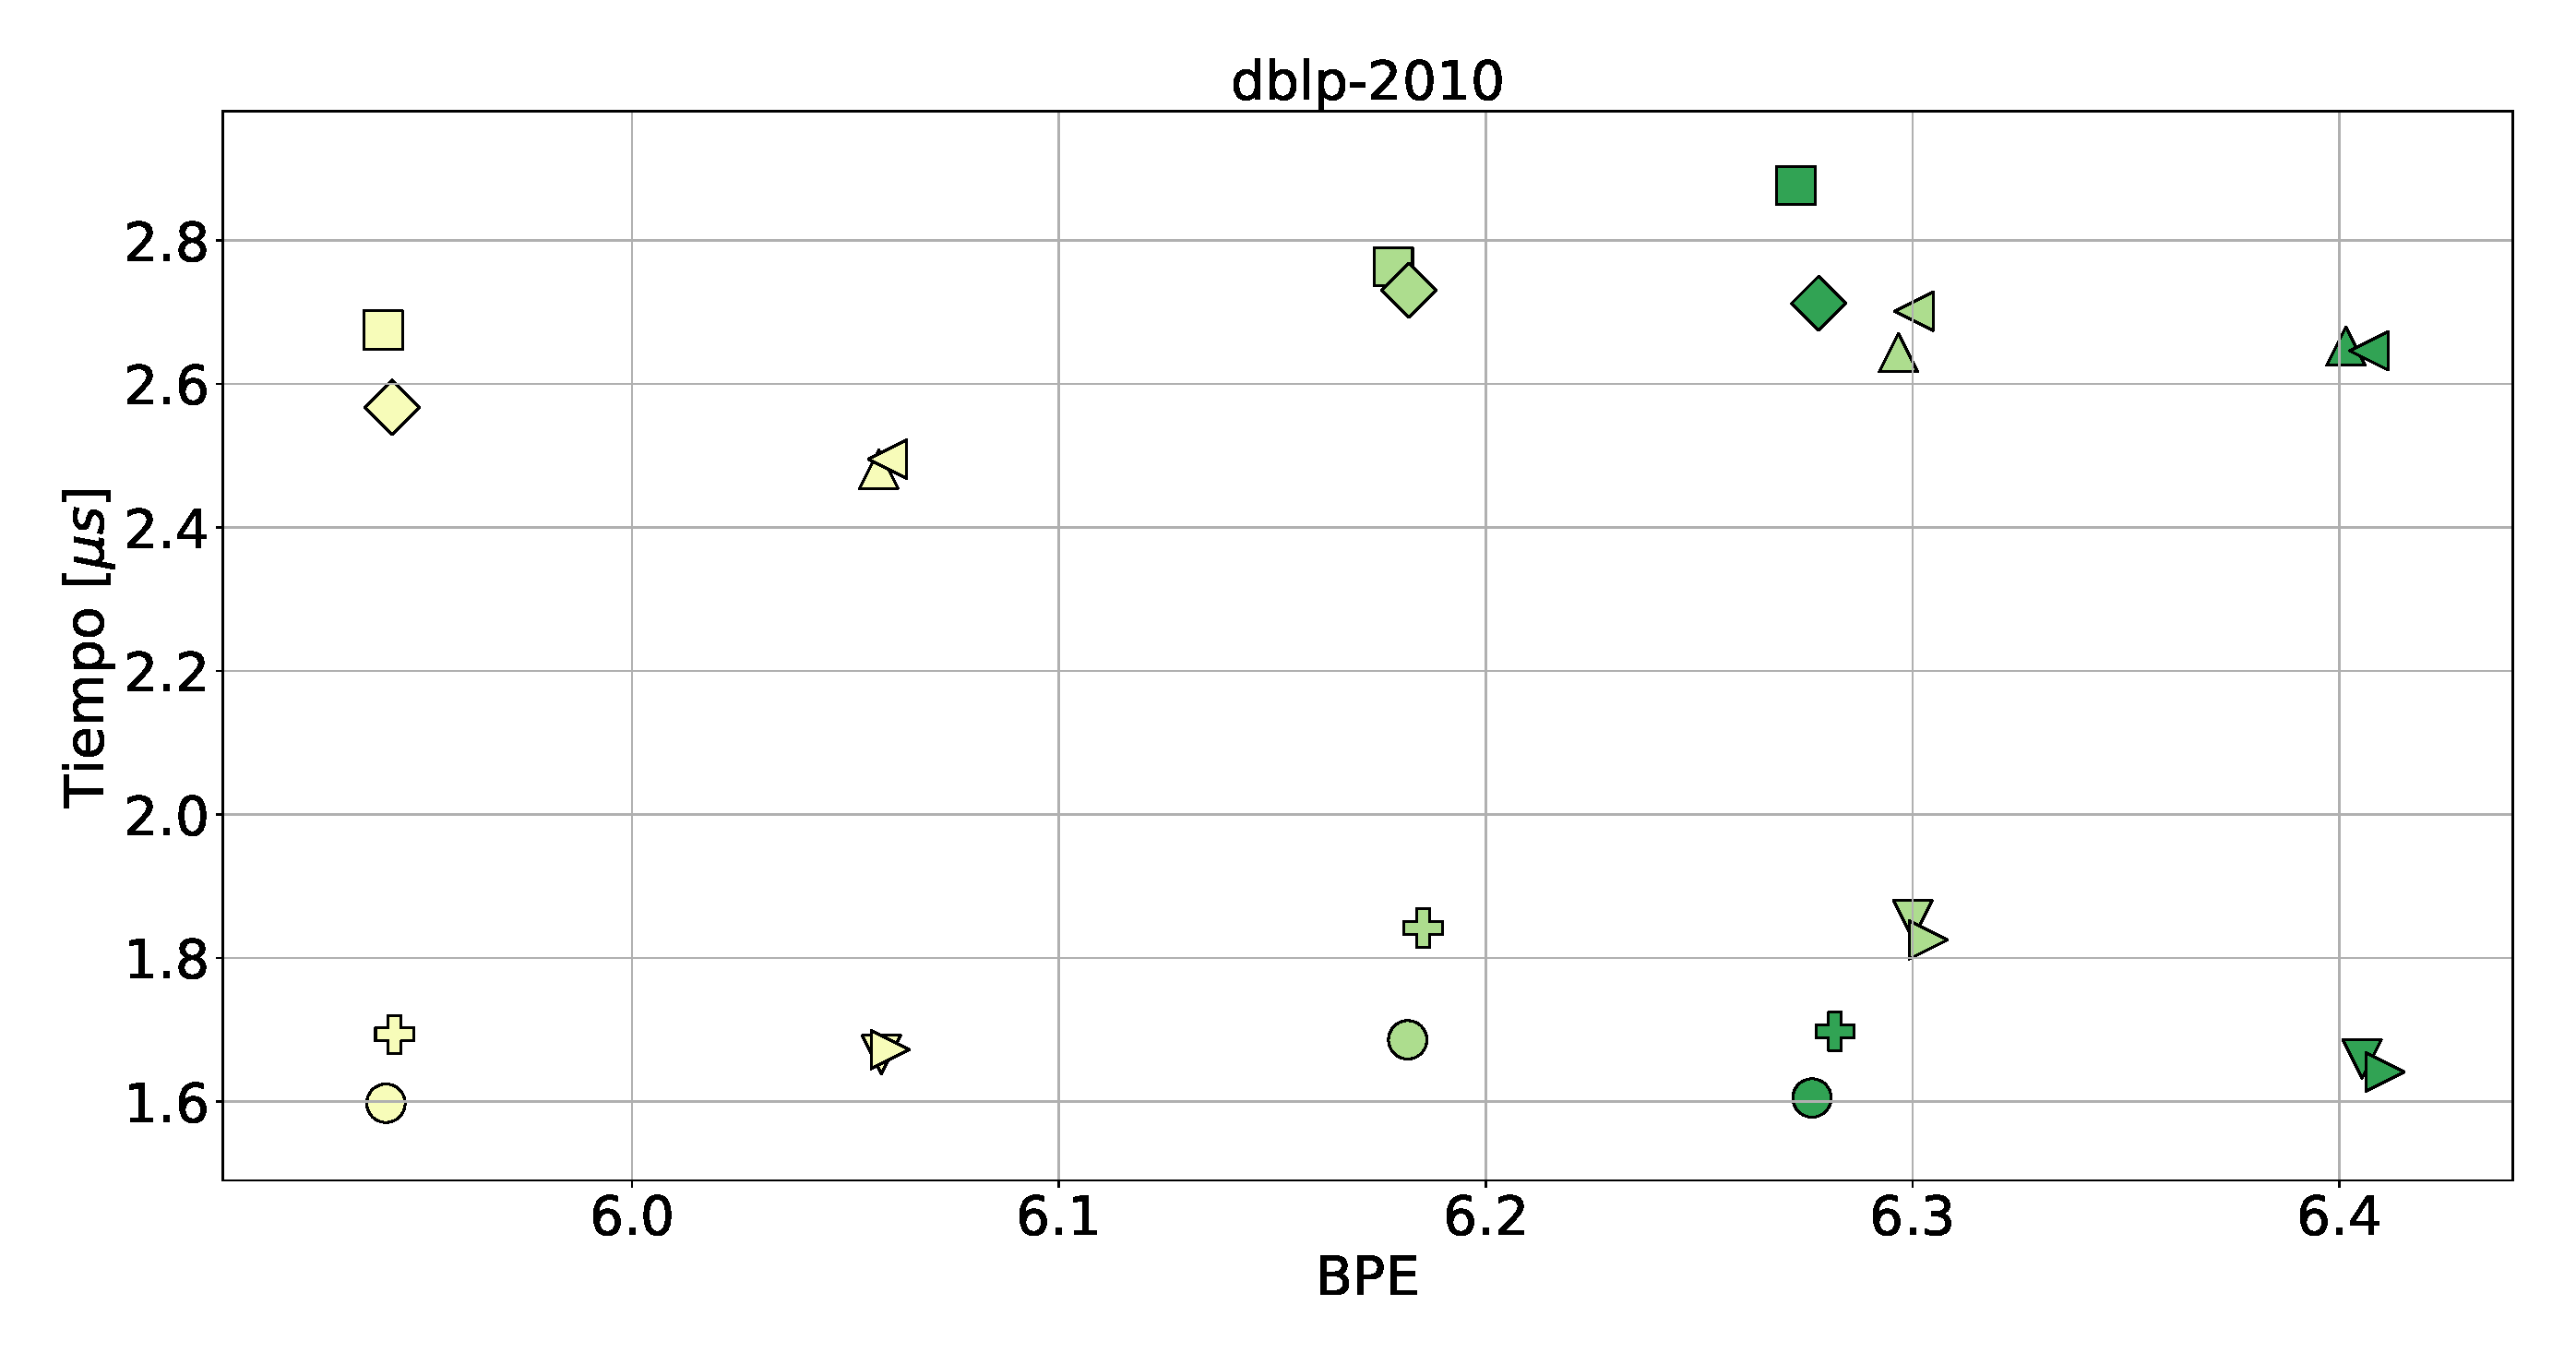
\includegraphics[width=1\linewidth]{../img/sdsl/secuencialBig/dblp-2010.pdf}
    		\end{minipage}
    		\begin{minipage}{0.15\textwidth}
    			\centering
    			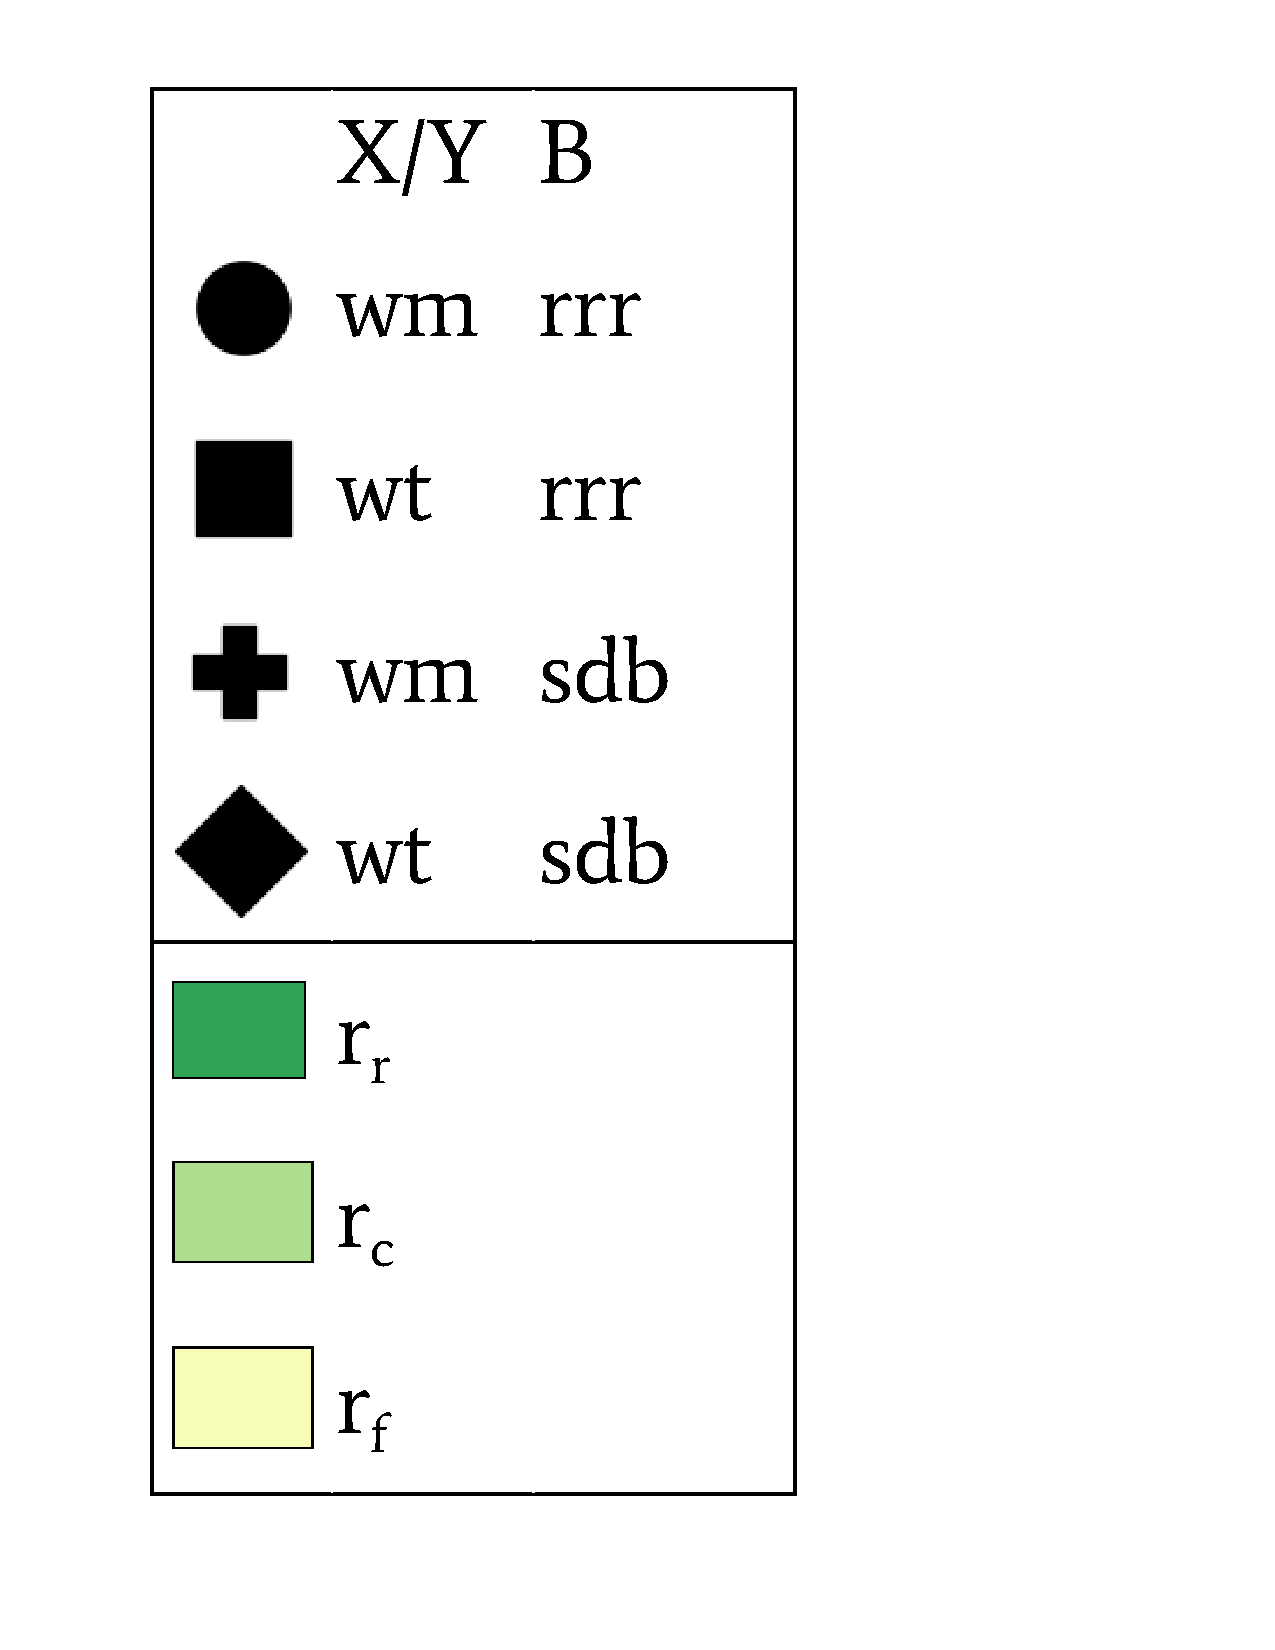
\includegraphics[scale=.15, clip, trim=70 0 0 0]{../img/sdsl/label.pdf}
    		\end{minipage}	
    	\end{minipage}

	\caption{BPE y Tiempo de acceso secuencial medio para posibles estructuras compactas, por cada función de ranking, para dblp-2010.}
\end{figure}

\end{frame}

\begin{frame}
\frametitle{Resultados - Estructura compacta}

\begin{figure}
	\centering
	
    	\begin{minipage}{1\textwidth}
    		\centering
    		\begin{minipage}{0.8\textwidth}
    			\centering
    			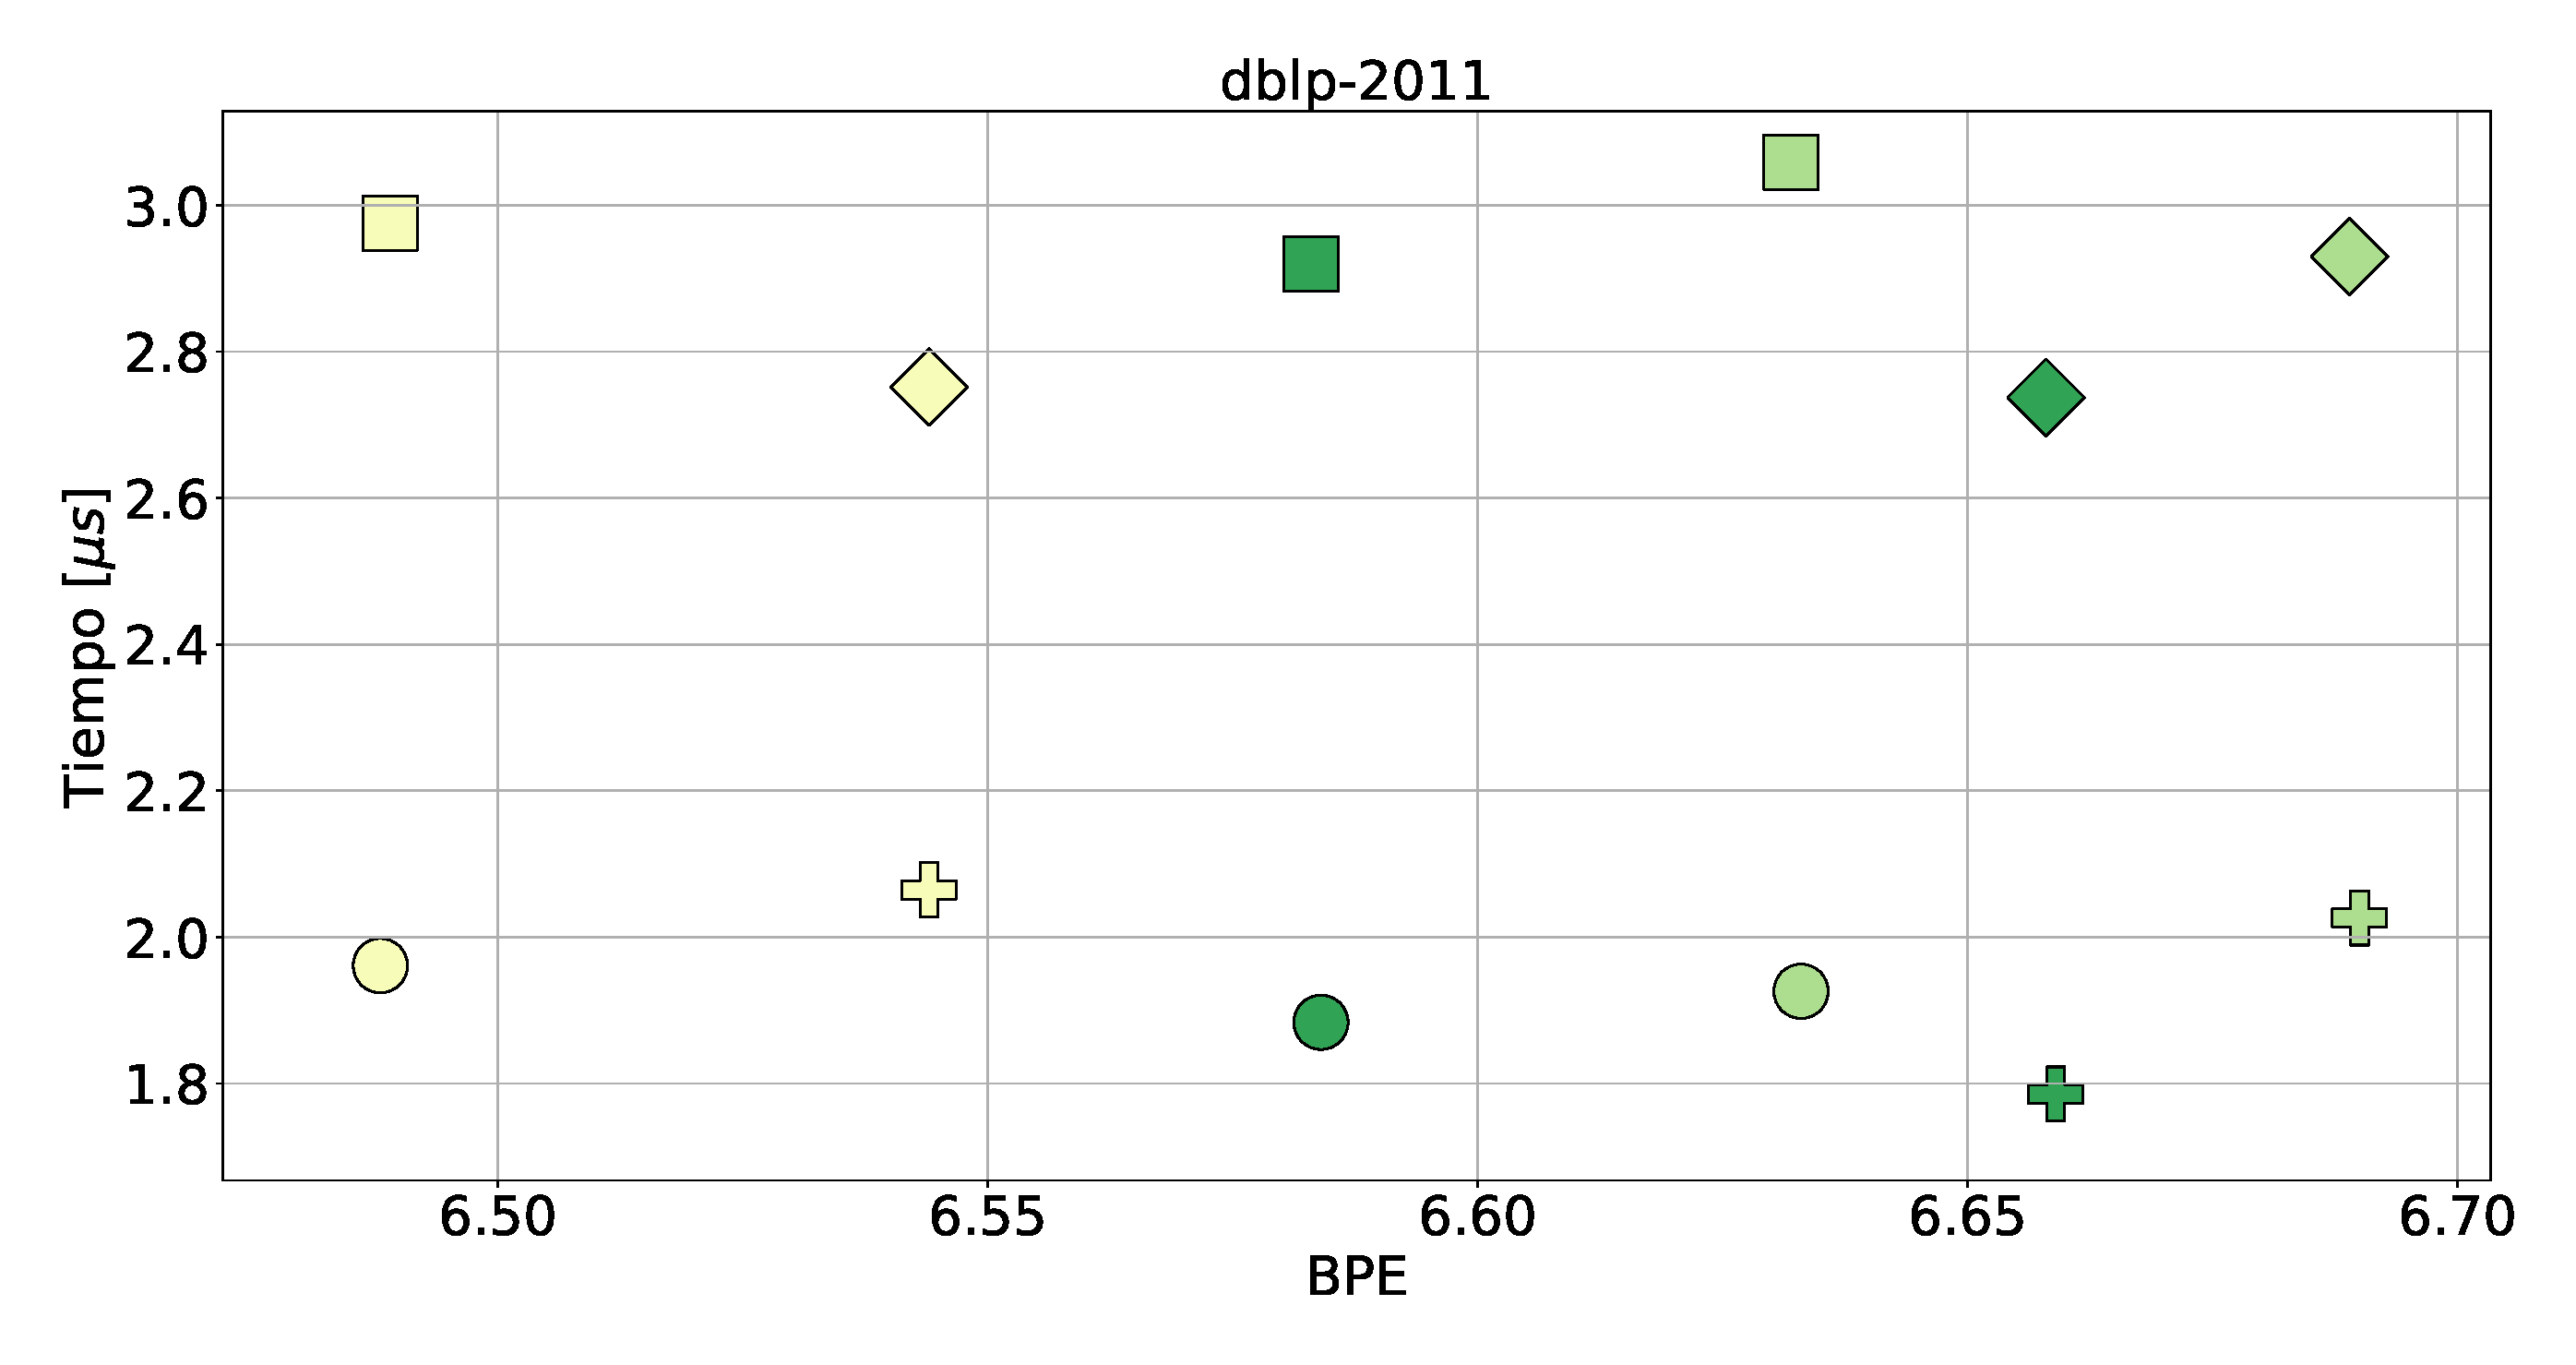
\includegraphics[width=1\linewidth]{../img/sdsl/secuencialBig/dblp-2011.pdf}
    		\end{minipage}
    		\begin{minipage}{0.15\textwidth}
    			\centering
    			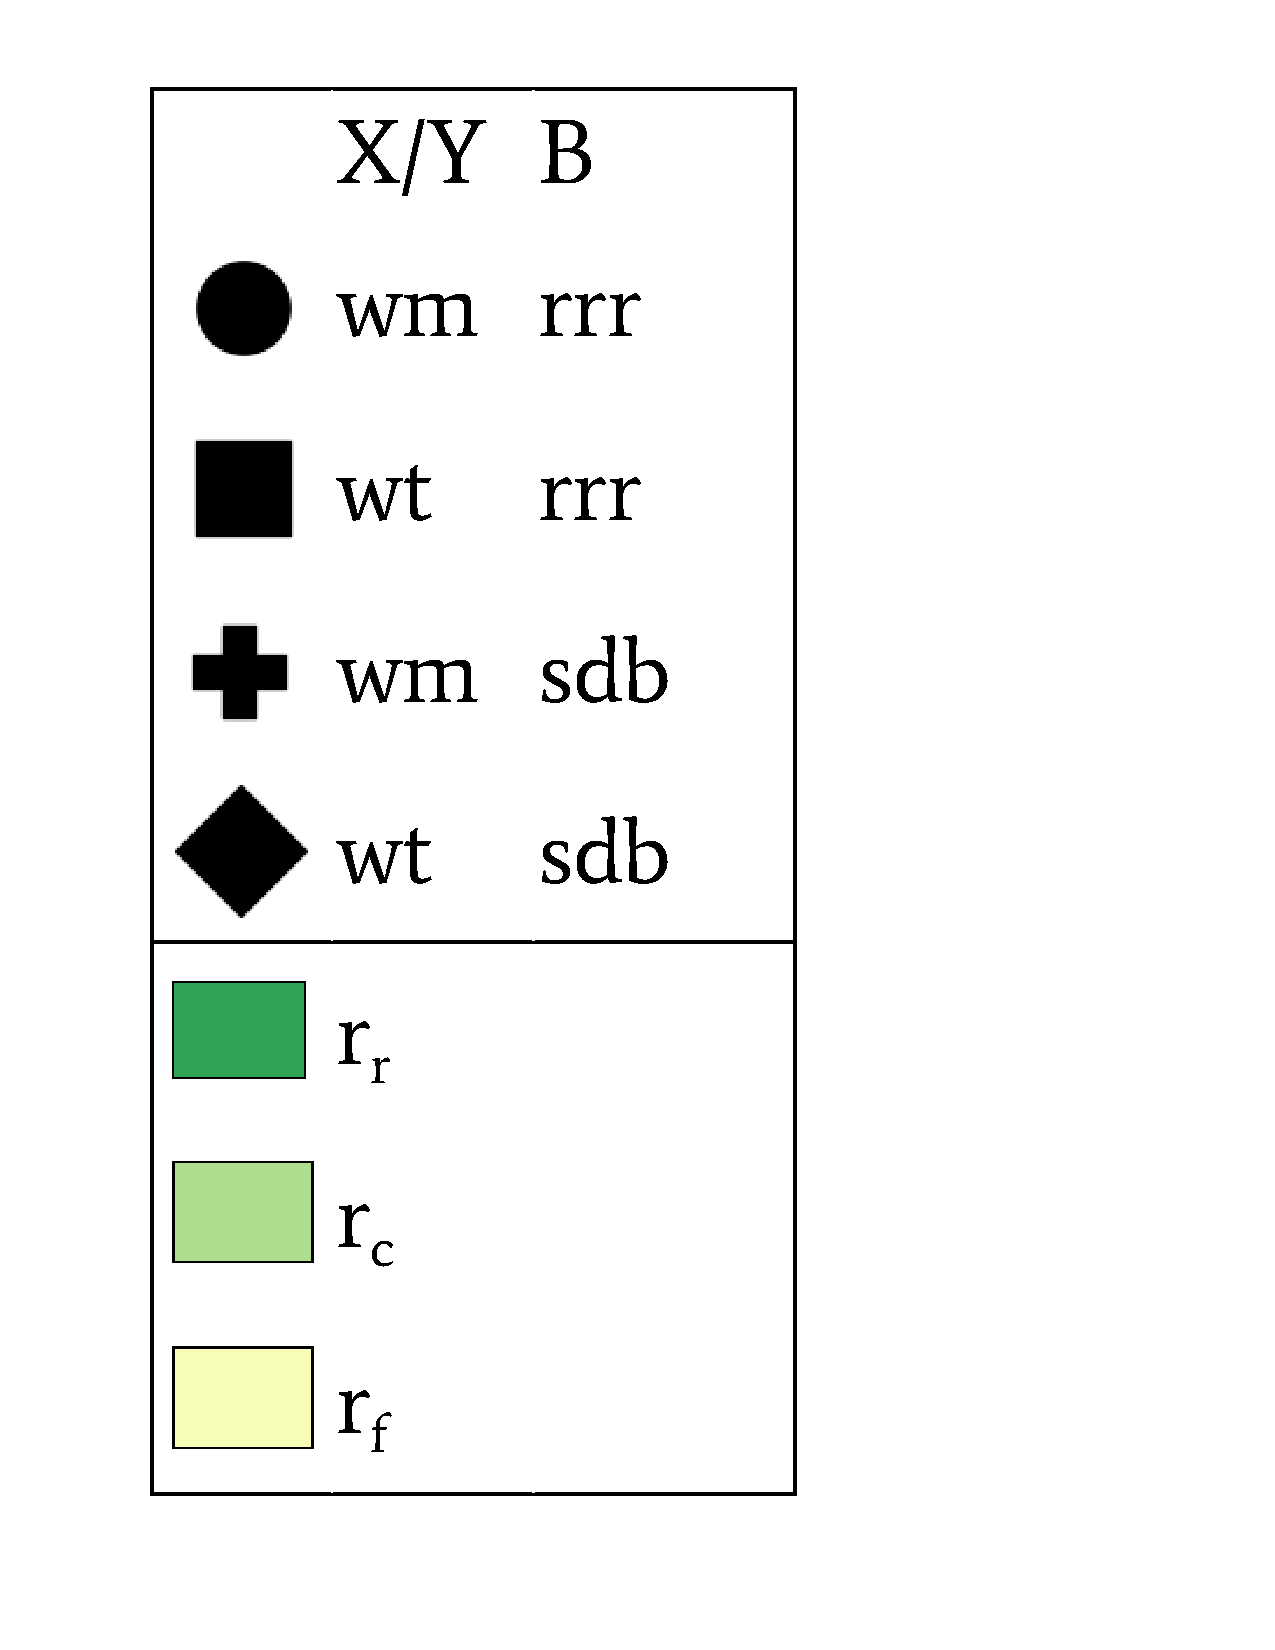
\includegraphics[scale=.15, clip, trim=70 0 0 0]{../img/sdsl/label.pdf}
    		\end{minipage}	
    	\end{minipage}

	\caption{BPE y Tiempo de acceso secuencial medio para posibles estructuras compactas, por cada función de ranking, para dblp-2011.}
\end{figure}

\end{frame}

\begin{frame}
\frametitle{Resultados - Estructura compacta}

\begin{figure}
	\centering
	
    	\begin{minipage}{1\textwidth}
    		\centering
    		\begin{minipage}{0.8\textwidth}
    			\centering
    			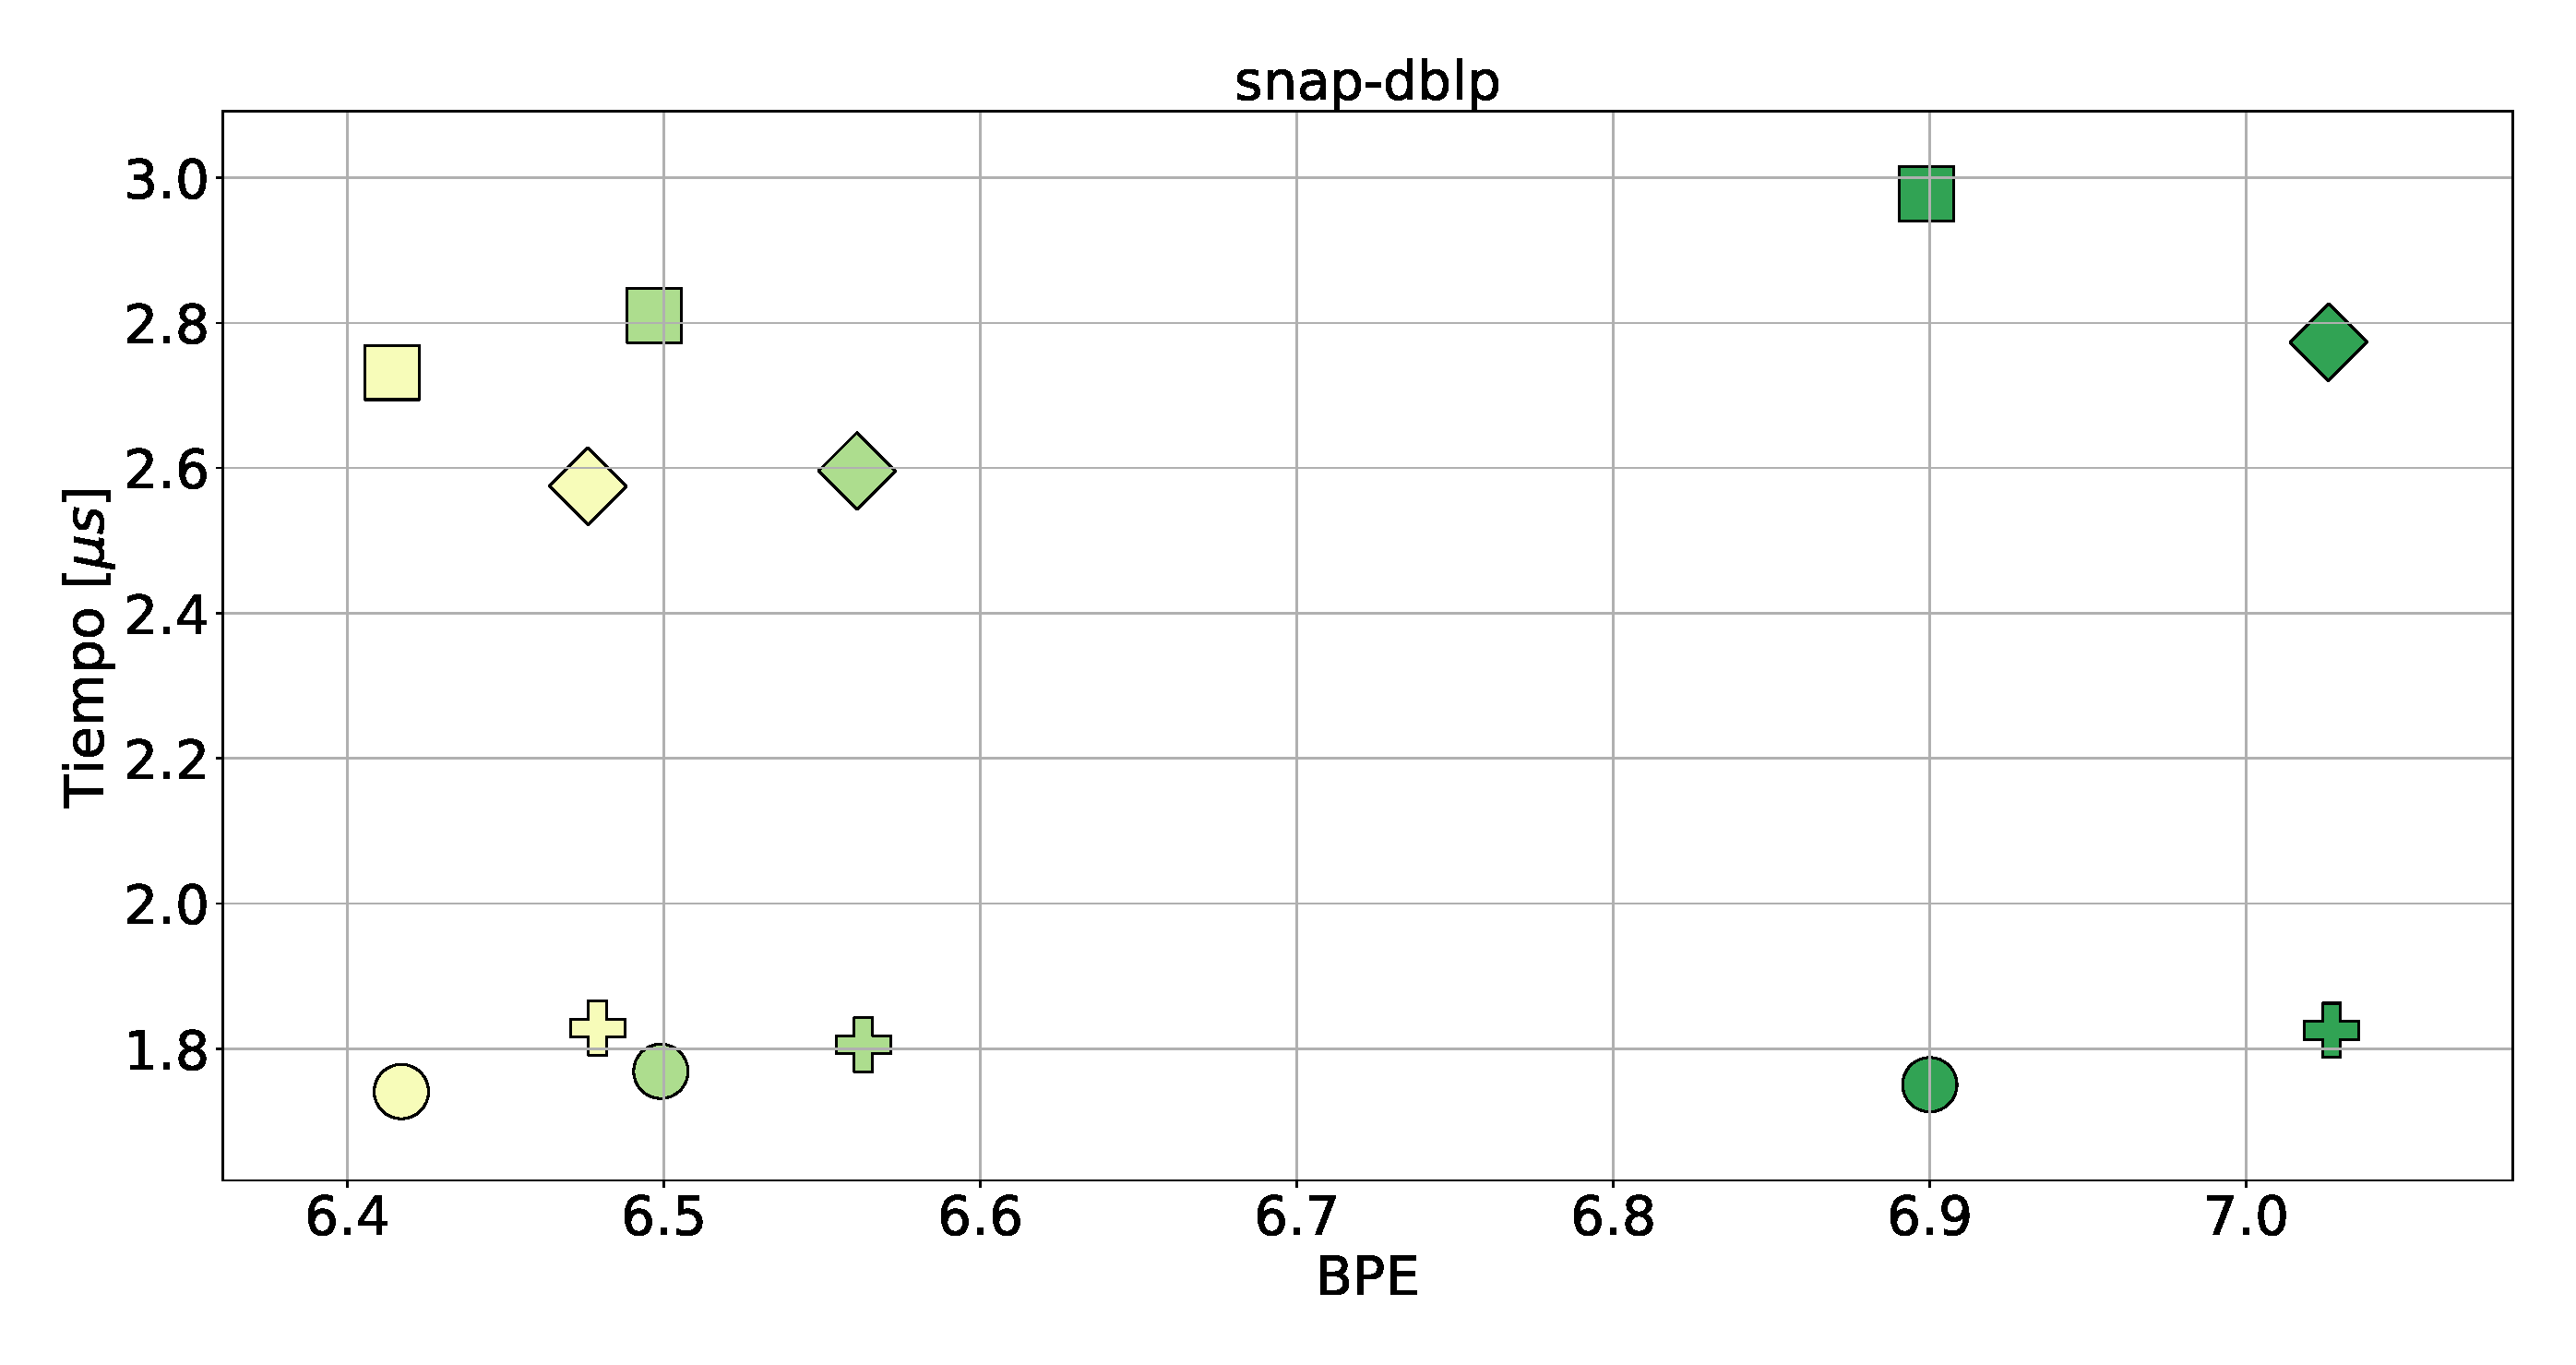
\includegraphics[width=1\linewidth]{../img/sdsl/secuencialBig/snap-dblp.pdf}
    		\end{minipage}
    		\begin{minipage}{0.15\textwidth}
    			\centering
    			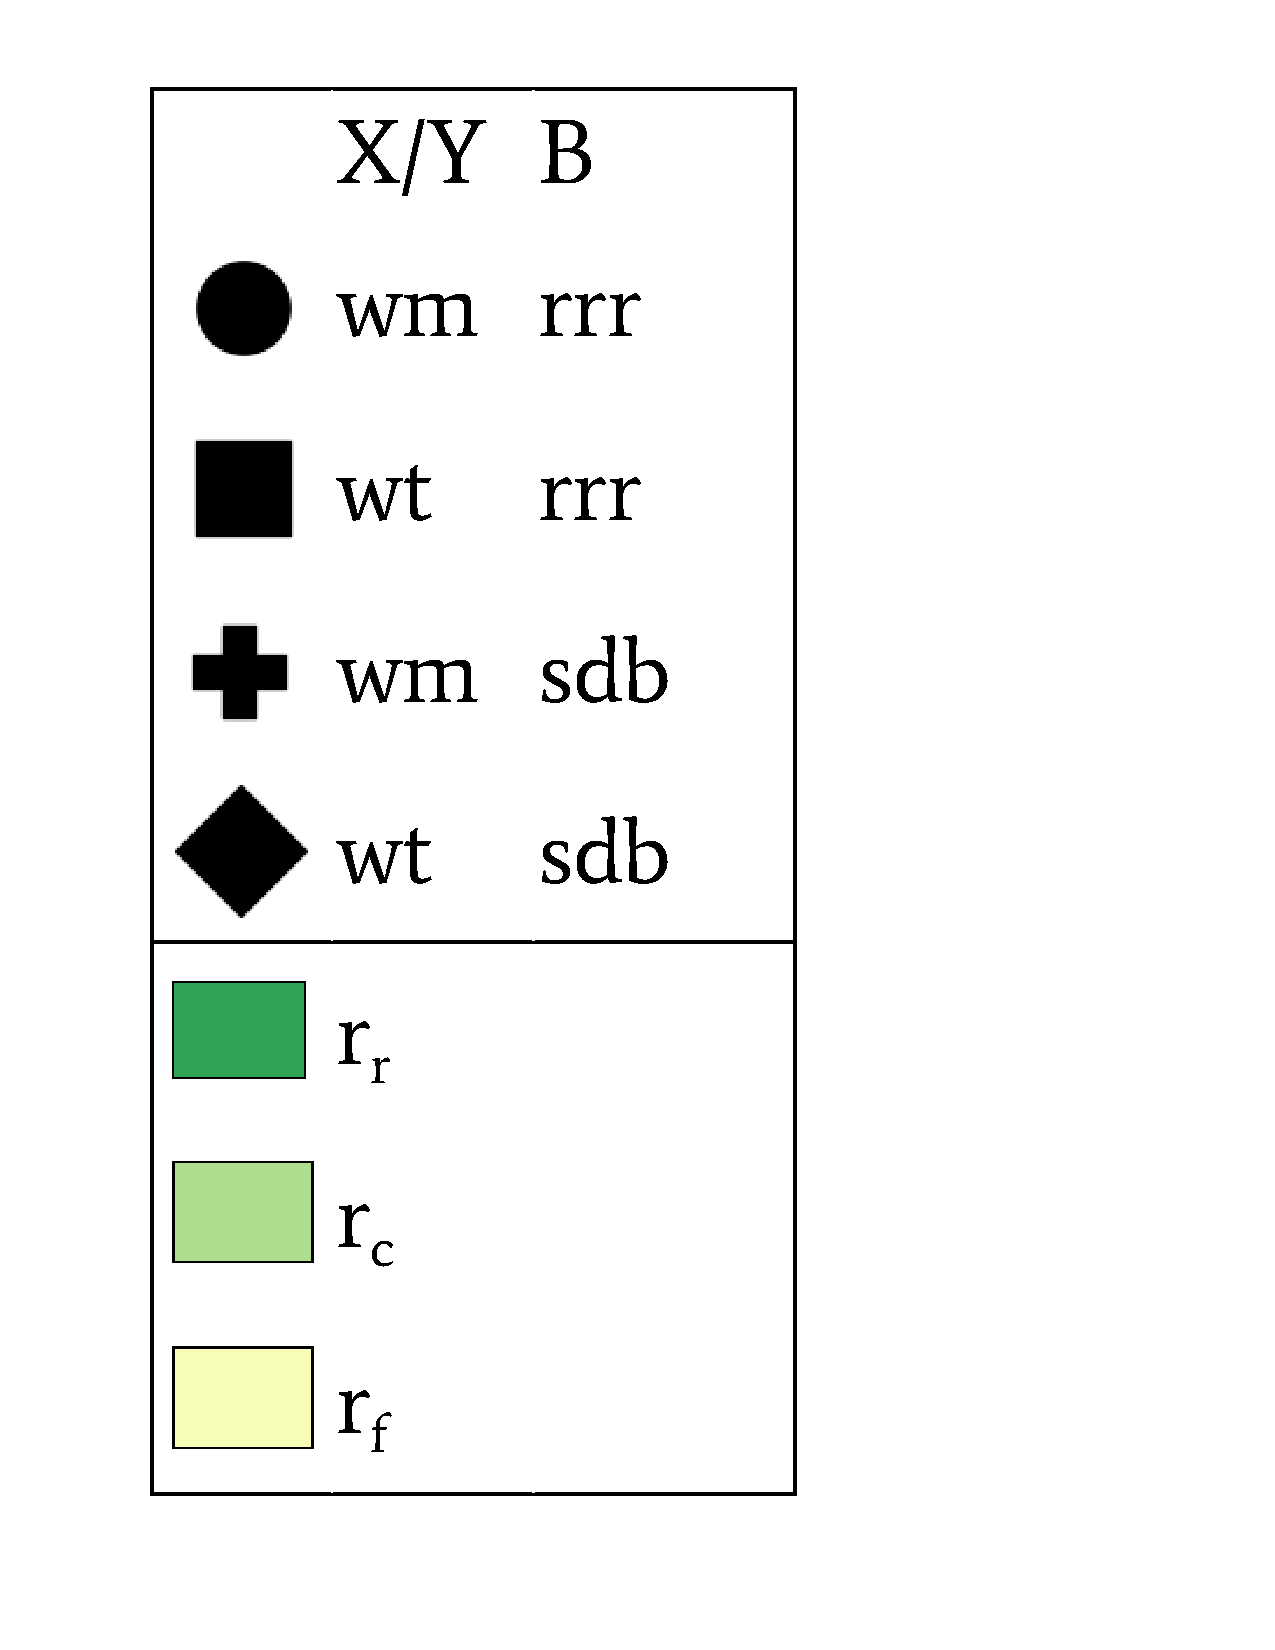
\includegraphics[scale=.15, clip, trim=70 0 0 0]{../img/sdsl/label.pdf}
    		\end{minipage}	
    	\end{minipage}

	\caption{BPE y Tiempo de acceso secuencial medio para posibles estructuras compactas, por cada función de ranking, para snap-dblp.}
\end{figure}

\end{frame}

\begin{frame}
\frametitle{Resultados - Estructura compacta}

\begin{figure}
	\centering
	
    	\begin{minipage}{1\textwidth}
    		\centering
    		\begin{minipage}{0.8\textwidth}
    			\centering
    			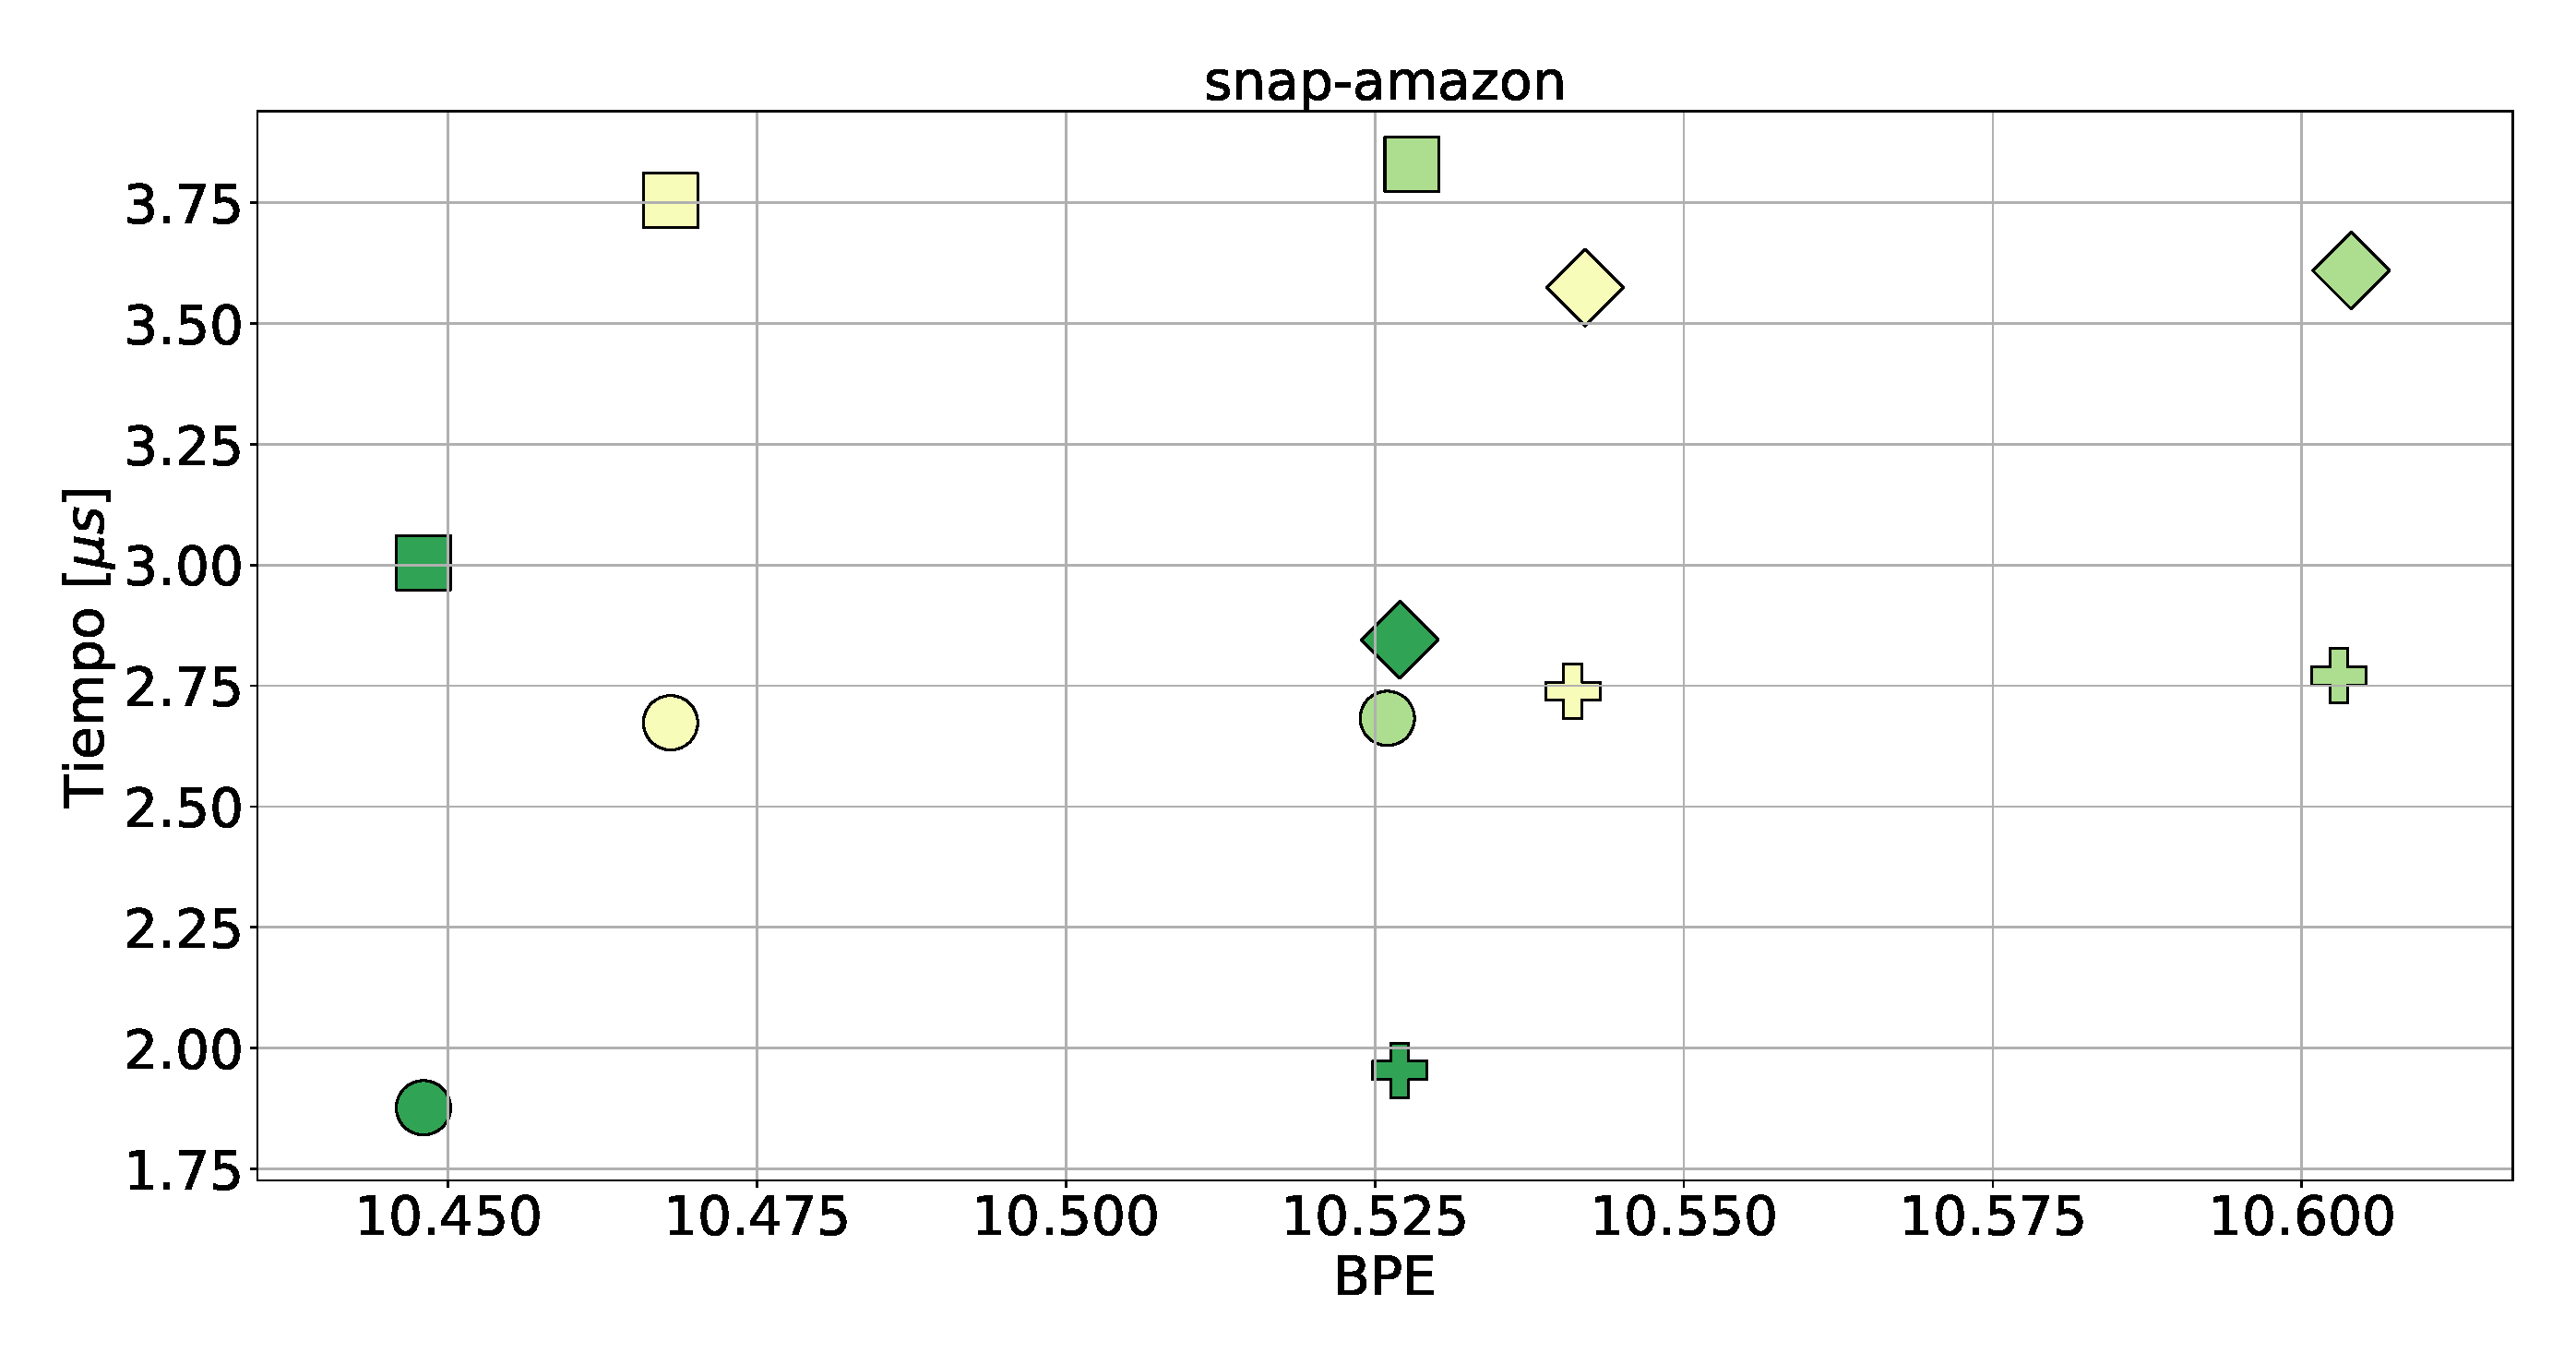
\includegraphics[width=1\linewidth]{../img/sdsl/secuencialBig/snap-amazon.pdf}
    		\end{minipage}
    		\begin{minipage}{0.15\textwidth}
    			\centering
    			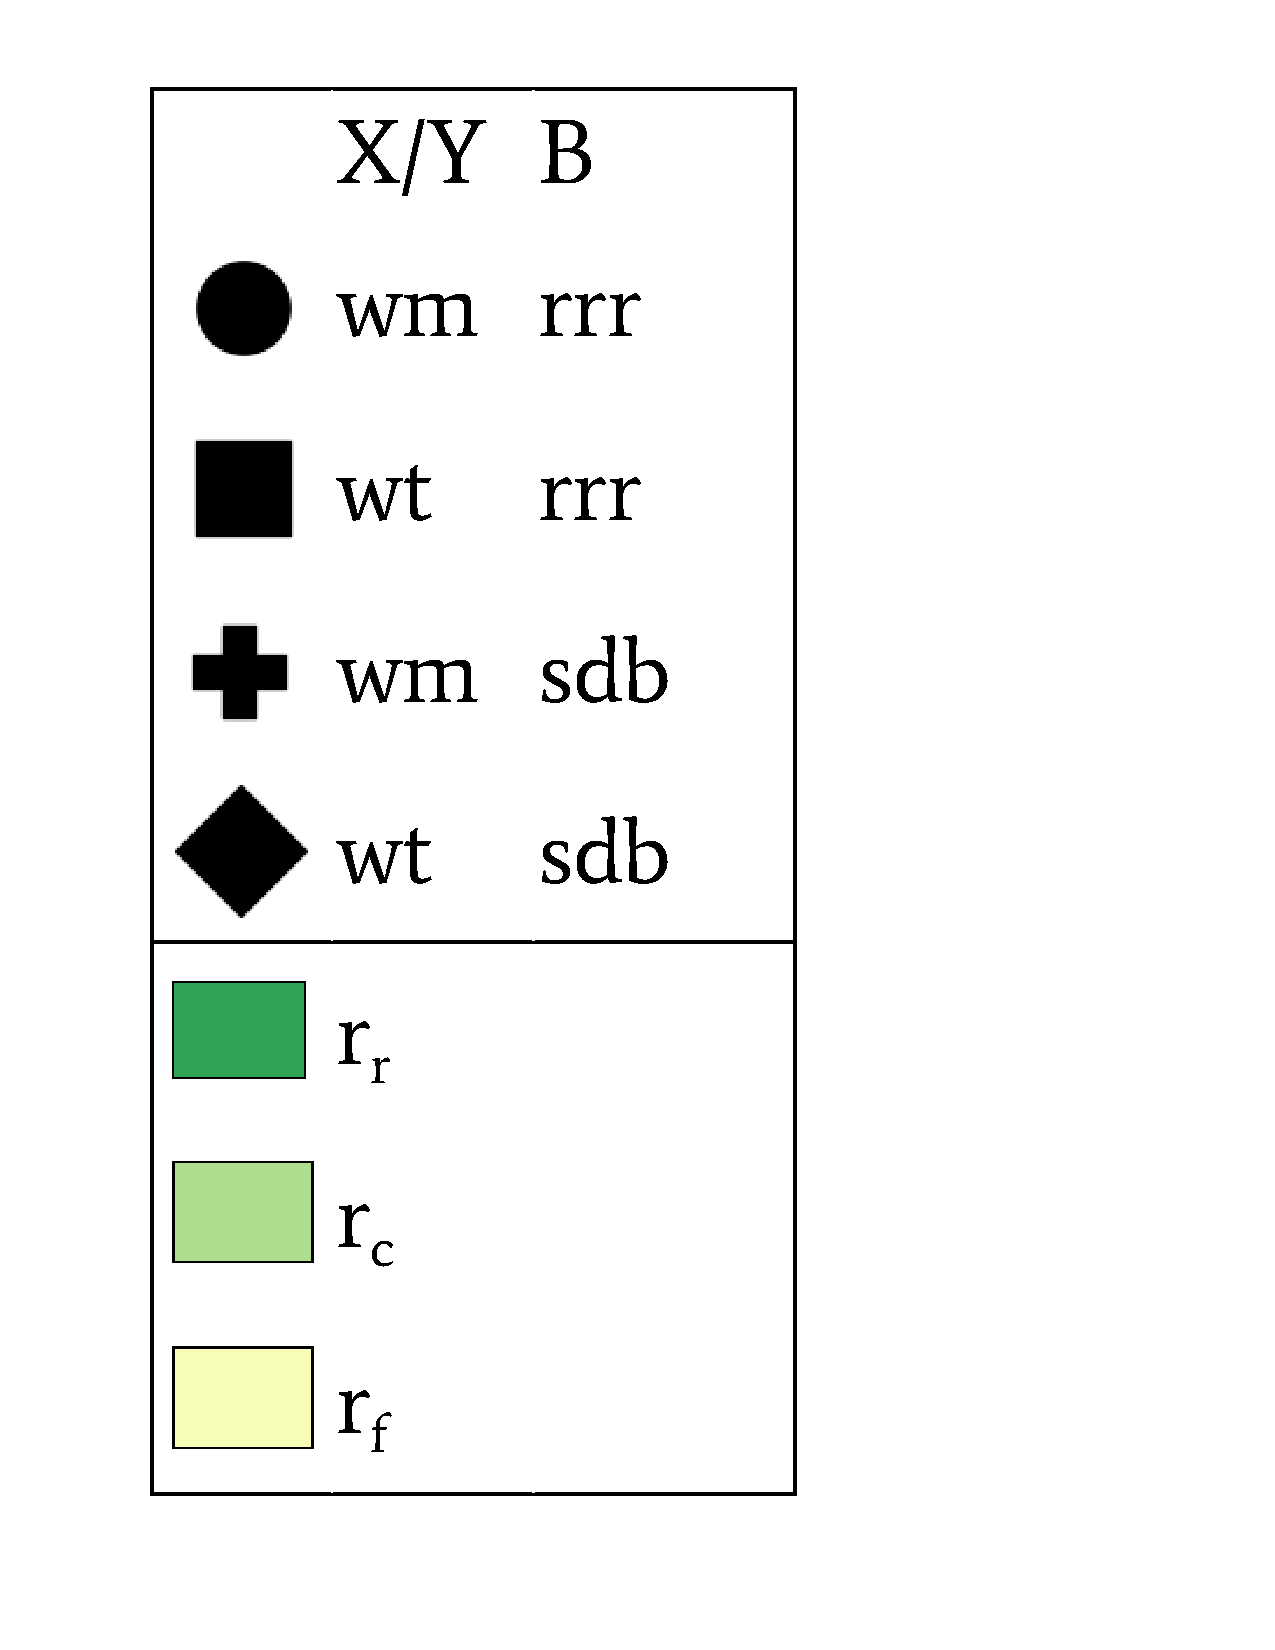
\includegraphics[scale=.15, clip, trim=70 0 0 0]{../img/sdsl/label.pdf}
    		\end{minipage}	
    	\end{minipage}

	\caption{BPE y Tiempo de acceso secuencial medio para posibles estructuras compactas, por cada función de ranking, para snap-amazon.}
\end{figure}

\end{frame}

\begin{frame}
\frametitle{Resultados - Estructura compacta}

\begin{figure}
	\centering
	
    	\begin{minipage}{1\textwidth}
    		\centering
    		\begin{minipage}{0.8\textwidth}
    			\centering
    			\includegraphics[width=1\linewidth]{../img/sdsl/secuencialBig/coPapersDBLP.pdf}
    		\end{minipage}
    		\begin{minipage}{0.15\textwidth}
    			\centering
    			\includegraphics[scale=.15, clip, trim=70 0 0 0]{../img/sdsl/label.pdf}
    		\end{minipage}	
    	\end{minipage}

	\caption{BPE y Tiempo de acceso secuencial medio para posibles estructuras compactas, por cada función de ranking, para coPapersDBLP.}
\end{figure}

\end{frame}

\begin{frame}
\frametitle{Resultados - Estructura compacta}

\begin{figure}
	\centering
	
    	\begin{minipage}{1\textwidth}
    		\centering
    		\begin{minipage}{0.8\textwidth}
    			\centering
    			\includegraphics[width=1\linewidth]{../img/sdsl/secuencialBig/coPapersCiteseer.pdf}
    		\end{minipage}
    		\begin{minipage}{0.15\textwidth}
    			\centering
    			\includegraphics[scale=.15, clip, trim=70 0 0 0]{../img/sdsl/label.pdf}
    		\end{minipage}	
    	\end{minipage}

	\caption{BPE y Tiempo de acceso secuencial medio para posibles estructuras compactas, por cada función de ranking, para coPapersCiteseer.}
\end{figure}

\end{frame}






\begin{frame}
\frametitle{Resultados - Comparando con estado del arte}

\begin{figure}
	\centering
	
    	\begin{minipage}{1\textwidth}
    		\centering
    		\begin{minipage}{0.8\textwidth}
    			\centering
    			\includegraphics[width=1\linewidth]{../img/bpeTimes/aleatorio/marknewman-astro.pdf}
    		\end{minipage}
    		\begin{minipage}{0.15\textwidth}
    			\centering
    			\includegraphics[scale=.16, clip, trim=70 200 280 40]{../img/bpeTimes/labelAle.pdf}
    		\end{minipage}	
    	\end{minipage}

	\caption{BPE y tiempo de acceso aleatorio en microsegundos de cada algoritmo, para marknewman-astro.}
\end{figure}

\end{frame}

\begin{frame}
\frametitle{Resultados - Comparando con estado del arte}

\begin{figure}
	\centering
	
    	\begin{minipage}{1\textwidth}
    		\centering
    		\begin{minipage}{0.8\textwidth}
    			\centering
    			\includegraphics[width=1\linewidth]{../img/bpeTimes/aleatorio/marknewman-condmat.pdf}
    		\end{minipage}
    		\begin{minipage}{0.15\textwidth}
    			\centering
    			\includegraphics[scale=.16, clip, trim=70 200 280 40]{../img/bpeTimes/labelAle.pdf}
    		\end{minipage}	
    	\end{minipage}

	\caption{BPE y tiempo de acceso aleatorio en microsegundoss de cada algoritmo, para marknewman-condmat.}
\end{figure}

\end{frame}

\begin{frame}
\frametitle{Resultados - Comparando con estado del arte}

\begin{figure}
	\centering
	
    	\begin{minipage}{1\textwidth}
    		\centering
    		\begin{minipage}{0.8\textwidth}
    			\centering
    			\includegraphics[width=1\linewidth]{../img/bpeTimes/aleatorio/dblp-2010.pdf}
    		\end{minipage}
    		\begin{minipage}{0.15\textwidth}
    			\centering
    			\includegraphics[scale=.16, clip, trim=70 200 280 40]{../img/bpeTimes/labelAle.pdf}
    		\end{minipage}	
    	\end{minipage}

	\caption{BPE y tiempo de acceso aleatorio en microsegundos de cada algoritmo, para dblp-2010.}
\end{figure}

\end{frame}

\begin{frame}
\frametitle{Resultados - Comparando con estado del arte}

\begin{figure}
	\centering
	
    	\begin{minipage}{1\textwidth}
    		\centering
    		\begin{minipage}{0.8\textwidth}
    			\centering
    			\includegraphics[width=1\linewidth]{../img/bpeTimes/aleatorio/dblp-2011.pdf}
    		\end{minipage}
    		\begin{minipage}{0.15\textwidth}
    			\centering
    			\includegraphics[scale=.16, clip, trim=70 200 280 40]{../img/bpeTimes/labelAle.pdf}
    		\end{minipage}	
    	\end{minipage}

	\caption{BPE y tiempo de acceso aleatorio en microsegundos de cada algoritmo, para dblp-2011.}
\end{figure}

\end{frame}

\begin{frame}
\frametitle{Resultados - Comparando con estado del arte}

\begin{figure}
	\centering
	
    	\begin{minipage}{1\textwidth}
    		\centering
    		\begin{minipage}{0.8\textwidth}
    			\centering
    			\includegraphics[width=1\linewidth]{../img/bpeTimes/aleatorio/snap-dblp.pdf}
    		\end{minipage}
    		\begin{minipage}{0.15\textwidth}
    			\centering
    			\includegraphics[scale=.16, clip, trim=70 200 280 40]{../img/bpeTimes/labelAle.pdf}
    		\end{minipage}	
    	\end{minipage}

	\caption{BPE y tiempo de acceso aleatorio en microsegundos de cada algoritmo, para snap-dblp.}
\end{figure}

\end{frame}

\begin{frame}
\frametitle{Resultados - Comparando con estado del arte}

\begin{figure}
	\centering
	
    	\begin{minipage}{1\textwidth}
    		\centering
    		\begin{minipage}{0.8\textwidth}
    			\centering
    			\includegraphics[width=1\linewidth]{../img/bpeTimes/aleatorio/snap-amazon.pdf}
    		\end{minipage}
    		\begin{minipage}{0.15\textwidth}
    			\centering
    			\includegraphics[scale=.16, clip, trim=70 200 280 40]{../img/bpeTimes/labelAle.pdf}
    		\end{minipage}	
    	\end{minipage}

	\caption{BPE y tiempo de acceso aleatorio en microsegundos de cada algoritmo, para snap-amazon.}
\end{figure}

\end{frame}

\begin{frame}
\frametitle{Resultados - Comparando con estado del arte}

\begin{figure}
	\centering
	
    	\begin{minipage}{1\textwidth}
    		\centering
    		\begin{minipage}{0.8\textwidth}
    			\centering
    			\includegraphics[width=1\linewidth]{../img/bpeTimes/aleatorio/coPapersDBLP.pdf}
    		\end{minipage}
    		\begin{minipage}{0.15\textwidth}
    			\centering
    			\includegraphics[scale=.16, clip, trim=70 200 280 40]{../img/bpeTimes/labelAle.pdf}
    		\end{minipage}	
    	\end{minipage}

	\caption{BPE y tiempo de acceso aleatorio en microsegundos de cada algoritmo, para coPapersDBLP.}
\end{figure}

\end{frame}

\begin{frame}
\frametitle{Resultados - Comparando con estado del arte}

\begin{figure}
	\centering
	
    	\begin{minipage}{1\textwidth}
    		\centering
    		\begin{minipage}{0.8\textwidth}
    			\centering
    			\includegraphics[width=1\linewidth]{../img/bpeTimes/aleatorio/coPapersCiteseer.pdf}
    		\end{minipage}
    		\begin{minipage}{0.15\textwidth}
    			\centering
    			\includegraphics[scale=.16, clip, trim=70 200 280 40]{../img/bpeTimes/labelAle.pdf}
    		\end{minipage}	
    	\end{minipage}

	\caption{BPE y tiempo de acceso aleatorio en microsegundos de cada algoritmo, para coPapersCiteseer.}
\end{figure}

\end{frame}





\begin{frame}
\frametitle{Resultados - Comparando con estado del arte}

\begin{figure}
	\centering
	
    	\begin{minipage}{1\textwidth}
    		\centering
    		\begin{minipage}{0.8\textwidth}
    			\centering
    			\includegraphics[width=1\linewidth]{../img/bpeTimes/secuencial/marknewman-astro.pdf}
    		\end{minipage}
    		\begin{minipage}{0.15\textwidth}
    			\centering
    			\includegraphics[scale=.16, clip, trim=70 200 280 40]{../img/bpeTimes/labelSec.pdf}
    		\end{minipage}	
    	\end{minipage}

	\caption{BPE y tiempo de reconstrucción secuencial en segundos de cada algoritmo, para marknewman-astro.}
\end{figure}

\end{frame}

\begin{frame}
\frametitle{Resultados - Comparando con estado del arte}

\begin{figure}
	\centering
	
    	\begin{minipage}{1\textwidth}
    		\centering
    		\begin{minipage}{0.8\textwidth}
    			\centering
    			\includegraphics[width=1\linewidth]{../img/bpeTimes/secuencial/marknewman-condmat.pdf}
    		\end{minipage}
    		\begin{minipage}{0.15\textwidth}
    			\centering
    			\includegraphics[scale=.16, clip, trim=70 200 280 40]{../img/bpeTimes/labelSec.pdf}
    		\end{minipage}	
    	\end{minipage}

	\caption{BPE y tiempo de reconstrucción secuencial en segundos de cada algoritmo, para marknewman-condmat.}
\end{figure}

\end{frame}

\begin{frame}
\frametitle{Resultados - Comparando con estado del arte}

\begin{figure}
	\centering
	
    	\begin{minipage}{1\textwidth}
    		\centering
    		\begin{minipage}{0.8\textwidth}
    			\centering
    			\includegraphics[width=1\linewidth]{../img/bpeTimes/secuencial/dblp-2010.pdf}
    		\end{minipage}
    		\begin{minipage}{0.15\textwidth}
    			\centering
    			\includegraphics[scale=.16, clip, trim=70 200 280 40]{../img/bpeTimes/labelSec.pdf}
    		\end{minipage}	
    	\end{minipage}

	\caption{BPE y tiempo de reconstrucción secuencial en segundos de cada algoritmo, para dblp-2010.}
\end{figure}

\end{frame}

\begin{frame}
\frametitle{Resultados - Comparando con estado del arte}

\begin{figure}
	\centering
	
    	\begin{minipage}{1\textwidth}
    		\centering
    		\begin{minipage}{0.8\textwidth}
    			\centering
    			\includegraphics[width=1\linewidth]{../img/bpeTimes/secuencial/dblp-2011.pdf}
    		\end{minipage}
    		\begin{minipage}{0.15\textwidth}
    			\centering
    			\includegraphics[scale=.16, clip, trim=70 200 280 40]{../img/bpeTimes/labelSec.pdf}
    		\end{minipage}	
    	\end{minipage}

	\caption{BPE y tiempo de reconstrucción secuencial en segundos de cada algoritmo, para dblp-2011.}
\end{figure}

\end{frame}

\begin{frame}
\frametitle{Resultados - Comparando con estado del arte}

\begin{figure}
	\centering
	
    	\begin{minipage}{1\textwidth}
    		\centering
    		\begin{minipage}{0.8\textwidth}
    			\centering
    			\includegraphics[width=1\linewidth]{../img/bpeTimes/secuencial/snap-dblp.pdf}
    		\end{minipage}
    		\begin{minipage}{0.15\textwidth}
    			\centering
    			\includegraphics[scale=.16, clip, trim=70 200 280 40]{../img/bpeTimes/labelSec.pdf}
    		\end{minipage}	
    	\end{minipage}

	\caption{BPE y tiempo de reconstrucción secuencial en segundos de cada algoritmo, para snap-dblp.}
\end{figure}

\end{frame}

\begin{frame}
\frametitle{Resultados - Comparando con estado del arte}

\begin{figure}
	\centering
	
    	\begin{minipage}{1\textwidth}
    		\centering
    		\begin{minipage}{0.8\textwidth}
    			\centering
    			\includegraphics[width=1\linewidth]{../img/bpeTimes/secuencial/snap-amazon.pdf}
    		\end{minipage}
    		\begin{minipage}{0.15\textwidth}
    			\centering
    			\includegraphics[scale=.16, clip, trim=70 200 280 40]{../img/bpeTimes/labelSec.pdf}
    		\end{minipage}	
    	\end{minipage}

	\caption{BPE y tiempo de reconstrucción secuencial en segundos de cada algoritmo, para snap-amazon.}
\end{figure}

\end{frame}

\begin{frame}
\frametitle{Resultados - Comparando con estado del arte}

\begin{figure}
	\centering
	
    	\begin{minipage}{1\textwidth}
    		\centering
    		\begin{minipage}{0.8\textwidth}
    			\centering
    			\includegraphics[width=1\linewidth]{../img/bpeTimes/secuencial/coPapersDBLP.pdf}
    		\end{minipage}
    		\begin{minipage}{0.15\textwidth}
    			\centering
    			\includegraphics[scale=.16, clip, trim=70 200 280 40]{../img/bpeTimes/labelSec.pdf}
    		\end{minipage}	
    	\end{minipage}

	\caption{BPE y tiempo de reconstrucción secuencial en segundos de cada algoritmo, para coPapersDBLP.}
\end{figure}

\end{frame}

\begin{frame}
\frametitle{Resultados - Comparando con estado del arte}

\begin{figure}
	\centering
	
    	\begin{minipage}{1\textwidth}
    		\centering
    		\begin{minipage}{0.8\textwidth}
    			\centering
    			\includegraphics[width=1\linewidth]{../img/bpeTimes/secuencial/coPapersCiteseer.pdf}
    		\end{minipage}
    		\begin{minipage}{0.15\textwidth}
    			\centering
    			\includegraphics[scale=.16, clip, trim=70 200 280 40]{../img/bpeTimes/labelSec.pdf}
    		\end{minipage}	
    	\end{minipage}

	\caption{BPE y tiempo de reconstrucción secuencial en segundos de cada algoritmo, para coPapersCiteseer.}
\end{figure}

\end{frame}
